\documentclass[11pt,a4paper]{report}
\usepackage{amssymb}
\usepackage{amsmath}
%\usepackage[notref,notcite]{showkeys}
\usepackage{amsthm}
\usepackage{makeidx}

%\oddsidemargin 0.5 in
%\textwidth = 435pt
%\textheight = 22.0 cm
%\hoffset = -1.cm
%\voffset = - 1.2cm
%\baselineskip = 22pt

\usepackage[hmargin={3cm,3cm},vmargin={4cm,3.5cm}]{geometry}

\usepackage[MeX]{polski}
\usepackage[utf8]{inputenc}
\usepackage[pdftex]{graphicx}
\usepackage{comment}
\usepackage{mleftright}
\usepackage{enumerate}
\usepackage{array}
\usepackage{tikz}
\usetikzlibrary{matrix}

 \usepackage[colorlinks=true,linkcolor=black]{hyperref}

\hypersetup{urlcolor=blue, citecolor=red}
%\usepackage{hyperref}

%   \textheight=8.2 true in
%    \textwidth=5.0 true in
%     \topmargin 30pt
%      \setcounter{page}{1}

\def\currentvolume{X}
 \def\currentissue{X}
  \def\currentyear{200X}
   \def\currentmonth{XX}
    \def\ppages{X--XX}


\newtheorem{theorem}{Twierdzenie}[section]
\newtheorem{corollary}[theorem]{Wniosek}
\newtheorem*{main}{Main Theorem}
\newtheorem{lemma}[theorem]{Lemat}
\newtheorem{proposition}[theorem]{Stwierdzenie}
\newtheorem{conjecture}[theorem]{Conjecture}
\newtheorem*{problem}{Problem}

\theoremstyle{definition}
\newtheorem{example}[theorem]{Przykład}
\newtheorem{definition}[theorem]{Definicja}
\newtheorem{remark}[theorem]{Uwaga}
\newtheorem*{notation}{Notation}

\newcommand{\tr}{\mathrm{tr}}
\newcommand{\str}{\mathrm{str}}
\newcommand{\ber}{\mathrm{ber}}
\newcommand{\I}{\mathbb{I}}
\newcommand{\im}{\mathrm{i}}
\newcommand{\eps}{\varepsilon}

% Pogrubienie w tabelach

\makeatletter
\newcommand{\thickhline}{%
    \noalign {\ifnum 0=`}\fi \hrule height 1pt
    \futurelet \reserved@a \@xhline
}
\newcolumntype{"}{@{\hskip\tabcolsep\vrule width 1pt\hskip\tabcolsep}}
\makeatother

\makeindex

\begin{document}

\begin{titlepage}
	\begin{center}
								
		%\vspace*{1cm}
								
		\LARGE \textbf{Uniwersytet Warszawski}\\
		\LARGE Wydział Fizyki\\[2cm]
		\LARGE{\textbf{Wojciech Fabjańczuk}}\\
		\LARGE{Nr albumu: 358624}\\[3cm]
		\Huge \textbf{Metody supergeometryczne \\i zastosowania w fizyce}\\[3cm]
		\Large Praca licencjacka\\
		na kierunku fizyka w ramach Studiów Indywidualnych \\[2cm]
								
	\end{center}
	\begin{flushright}
		\Large Praca wykonana pod kierunkiem\\
		\textbf{dr Javiera de Lucas Araujo}\\
		Katedra Metod Matematycznych Fizyki\\[3.5cm]
	\end{flushright}
	\begin{center}
		\Large Warszawa, wrzesień 2017 r.
	\end{center}
\end{titlepage}

\noindent\textit{Oświadczenie kierującego pracą}\\[0.25cm]
\textnormal{Oświadczam, że niniejsza praca została przygotowana pod moim kierunkiem i stwierdzam, że spełnia ona warunki do przedstawienia jej w postępowaniu o nadanie tytułu zawodowego.}\\[1cm]

\noindent \hspace{1cm} \textnormal{Data} \hspace{2cm} \textnormal{Podpis kierującego pracą}
\\[4cm]

\noindent \textit{Oświadczenie autora (autorów) pracy}\\[0.25cm]
\textnormal{Świadom odpowiedzialności prawnej oświadczam, że niniejsza praca dyplomowa została napisana przeze mnie samodzielnie i nie zawiera treści uzyskanych w sposób niezgodny z obowiązującymi przepisami.\\ Oświadczam również, że przedstawiona praca nie była wcześniej przedmiotem procedur związanych z uzyskaniem tytułu zawodowego w wyższej uczelni.\\ Oświadczam ponadto, że niniejsza wersja pracy jest identyczna z załączoną wersją elektroniczną.}\\[1cm]

\noindent \hspace{1cm} \textnormal{Data} \hspace{2cm} \textnormal{Podpis autora (autorów) pracy}

\newpage

\begin{center}
	\textbf{Streszczenie}
\end{center}
\textnormal{Celem pracy jest omówienie geometrii superrozmaitości i przedstawienie zastosowania metod supergeometrycznych w fizyce. Przedstawiono opracowanie matematycznych aspektów supergeometrii i przytoczono wiele przykładów z supermechaniki, w tym opis superoscylatora harmonicznego i nierelatywistycznej, klasycznej cząstki ze spinem. Dodano niezbędną literaturę z zakresu badanej dziedziny. Tekst skierowany jest do studentów indywidualnych fizyki trzeciego roku lub studentów drugiego stopnia zainteresowanych podstawami matematycznymi supersymetrii.}

\vspace{2cm}

\begin{center}
	\textbf{Słowa kluczowe}\\[0.5cm]
	\textit{superprzestrzeń, superalgebra, berezinian, supergeometria,  superrozmaitość, supermechanika, superlagranżjan, superrównania Eulera-Lagrange'a, superhamiltonian, superrównania Hamiltona}
\end{center}
\vspace{2cm}

\begin{center}
	\textbf{Dziedzina pracy (kody wg programu Socrates-Erasmus)}\\[0.5cm]
	\textnormal{13.2 \ Fizyka}
\end{center}
\vspace{2cm}

\begin{center}
	\textbf{Tytuł pracy w języku angielskim}\\[0.5cm]
	\textnormal{Supergeometric methods and applications in physics}
\end{center}

\newpage
\tableofcontents

\newpage
\chapter*{Wstęp}
\addcontentsline{toc}{chapter}{Wstęp}
Teoria supergeometrii pojawiła się w fizyce wraz z ideą opisu fermionów w kwantowej teorii pola za pomocą antyprzemiennych potencjałów \cite{schmitt} i w teorii strun \cite{GS71,Sc12}. Supergeometria jest matematyczną teorią pozwalającą sformalizować różniczkowanie, całkowanie i wszystkie niezbędne operacje na nowych obiektach. W tym celu rozszerza się geometrię różniczkową o specjalne zmienne, których iloczyn po zmianie kolejności zmienia znak.

Teoria supergeometrii jest przede wszystkim podstawą wielu dziedzin fizyki teoretycznej takich jak supermechanika klasyczna \cite{carinena} i teorie supersymetryczne \cite{carmeli}, oraz znajduje zastosowanie w rozwiązywaniu niektórych problemów matematycznych w fizyce teoretycznej -- na przykład w kwantyzacji metodą całek po trajektoriach nieabelowych teorii pola z cechowaniem \cite{ryder}. Matematyków nie związanych z fizyką może zainteresować supersymetryczny dowód nierówności Morse'a \cite{witten}, jak również supersymetryczne wyprowadzenia różnych twierdzeń o indeksie \cite{alvarez, manes} i dużo różnych nieprzemiennych analogii struktur pojawiających się w geometrii różniczkowej \cite{cattaneo}.

Celem niniejszej pracy jest szczegółowe przedstawienie i skrupulatna analiza kluczowych pojęć supergeometrii od strony matematycznej, i ukazanie jej zastosowań w supermechanice klasycznej. Praca skierowana jest dla studentów fizyki indywidualnej trzeciego roku lub studentów lubiących algebrę, będących po kursie geometrii różniczkowej i zainteresowanych teoriami supersymetrycznymi z matematycznego punktu widzenia.

Formalizm teorii przedstawiono w autorski sposób -- drobiazgowy, ale możliwie najprostszy. Definicje i twierdzenia uzupełniono wieloma przykładami, czasami fizycznymi, czasami czysto teoretycznymi. W bibliografii na końcu pracy zamieszczono podstawową literaturę związaną z poruszonymi tematami.

Praca składa się z trzech rozdziałów: o superalgebrze liniowej, o supergeometrii i superrozmaitościach, o formalizmie superlagranżowskim i superhamiltonowskim w supermechanice klasycznej.

Pierwszy rozdział skupia się na algebraicznym wprowadzeniu do supergeometrii i prowadzi do definicji berezinianu (superwyznacznika) poprzez naturalne rozszerzenia obiektów algebry liniowej: superprzestrzenie, superalgebry, supermoduły i supermacierze.

W drugim rozdziale zaprezentowano istotę supergeometrii -- superrozmaitości, czyli uogólnienie rozmaitości różniczkowych w których lokalną algebrę funkcji gładkich zastąpiono algebrą Grassmanna. Opisano wiele innych uogólnień pojęć geometrii różniczkowej takich jak współrzędne, wiązka styczna, całkowanie.

Ostatni rozdział poświęcono supermechanice klasycznej, która odzwierciedla jedno z zastosowań supergeometrii w fizyce teoretycznej. Scharakteryzowano formalizm superlagranżowski i superhamiltonowski oraz pokazano sporo przykładów.

\newpage
\chapter*{Oznaczenia}
\addcontentsline{toc}{chapter}{Oznaczenia}

\begin{equation*}
	\begin{aligned}
		M                                              & :\quad \mathrm{rozmaitość\ różniczkowa\ }m\mathrm{-wymiarowa}                                                                                              \\
		\mathbb{N}                                     & :\quad \mathrm{zbiór\ liczb\ całkowitych\ większych\ od\ zera}                                                                                              \\
		\mathbb{Z}_+\!                                 & :\quad \mathrm{zbiór\ liczb\ całkowitych\ nieujemnych}                                                                                                       \\
		\mathbb{K}                                     & :\quad \textrm{ciało liczb rzeczywistych albo zespolonych}                                                                                                    \\
		\textrm{End}_{\mathbb{K}}(V)                   & :\quad \textrm{zbiór endomorfizmów przestrzeni wektorowej}\ V\ \textrm{nad}\ \mathbb{K}                                                                      \\
		\textrm{Id}_V                                  & :\quad \textrm{odwzorowanie tożsamościowe w przestrzeni wektorowej}\ V\ \textrm{nad}\ \mathbb{K}                                                             \\
		\check{f}                                      & :\quad \textrm{dla funkcji liniowej}\ f: X \rightarrow Y\ \textrm{funkcja taka, że}\ \forall x \in X,\ \check{f}(x) := f(-x)                                  \\
		W^{\circ}                                      & :\quad \textrm{zbiór}\ \omega \in V^*\ \textrm{spełniających}\ \forall x \in W,\ \omega (x) = 0                                                             \\
		\overline{m,n}                                 & : \quad \textrm{zbiór liczb całkowitych\ } z \textrm{\ spełniających }  m \leq z \leq n \textrm{\ dla } m,n \in \mathbb{Z},\ m \leq n                      \\
		\lfloor m \rfloor\ (\lceil m \rceil)           & : \quad \textrm{największa (najmniejsza) liczba całkowita nie większa (mniejsza) niż\ } m \in \mathbb{R}                                                   \\
		\Gamma(E)                                      & : \quad \textrm{cięcia wiązki wektorowej }E                                                                                                                  \\
		\Omega(M)                                      & : \quad \textrm{zbiór form różniczkowych nad rozmaitością }M                                                                                              \\
		\mathrm{Grass}(\mathbb{K}, L)                  & : \quad \textrm{algebra Grassmanna nad ciałem } \mathbb{K} \textrm{ o } L \textrm{ generatorach nieparzystych}                                                \\
		\underline \lambda                             & : \quad \textrm{multi-indeks}                                                                                                                                  \\
		\mathfrak{m}(\underline \lambda)               & : \quad \textrm{długość multi-indeksu } \lambda                                                                                                             \\
		\mathfrak{M}^L                                 & : \quad \textrm{zbiór multi-indeksów długości nie większej niż }L                                                                                        \\
		\underline \lambda ^c                          & : \quad \textrm{multi-indeks dopełniający do }\underline \lambda                                                                                             \\
		\beta_{\left[\, \underline{\lambda}\, \right]} & : \quad \textrm{iloczyn generatorów }\beta_{\lambda_1} \ldots \beta_{\lambda_k} \textrm{ dla multi-indeksu }\underline{\lambda} := \lambda_1,\ldots,\lambda_k \\
		\mathrm{Mat}(R,m,n)                            & : \quad \textrm{zbiór macierzy wymiaru } m \times n \textrm{ o elementach z }R                                                                                \\
		H^\infty(U)                                    & : \quad \mathrm{zbiór\ funkcji\ holomorficznych\ na\ otwartym\ } U                                                                                            \\
		\mathcal{M}                                    & : \quad \textrm{superrozmaitość o superwymiarze } (m,n)                                                                                                      \\
		C^\infty(\mathcal{M})                          & : \quad \mathrm{zbiór\ superfunkcji\ nad\ } \mathcal M                                                                                                        \\
		\mathcal{TM}                                   & : \quad \textrm{superrozmaitość styczna do }\mathcal{M}                                                                                                      \\
		\mathfrak X(\mathcal M)                        & : \quad \textrm{zbiór superpól wektorowych na }\mathcal{M}                                                                                                   \\
		\mathcal{T^*M}                                 & : \quad \textrm{superrozmaitość kostyczna do }\mathcal{M}                                                                                                    \\
		\Omega(\mathcal{M})                            & : \quad \textrm{zbiór superform różniczkowych na }\mathcal{M}                                                                                               \\
	\end{aligned}
\end{equation*}

\chapter{Superalgebra}

Niniejszy rozdział jest niezbędny do zrozumienia supergeometrii i supermechaniki. Przedstawiono najważniejsze z praktycznego punktu widzenia pojęcia superalgebry liniowej, jednak dziedzina ta jest rozleglejsza i atrakcyjna sama w sobie \cite{Co12,Du08,KT99,LZ17,Sa08,Tr99}.

Celem superalgebry liniowej jest badanie własności struktur algebraicznych z tak zwaną $\mathbb{Z}_2$-gradacją, w szczególności superprzestrzeni wektorowych, superalgebr i supermodułów, oraz ich morfizmów \cite{leites,rogers}.
W pracy będzie się domyślnie zakładać, że wszystkie rozważane odwzorowania są gładkie, chyba że zaznaczono inaczej. Przez algebry będzie się rozumieć algebry łączne z jedynką. Pojawiające się ciało $\mathbb{K}$ będzie zawsze albo ciałem liczb rzeczywistych, albo ciałem liczb zespolonych.

Dyskusję odwracalności homomorfizmów supermodułów, aksjomatyczną definicję berezinianu, dowód jego istnienia oraz jedyności przeprowadzono tak jak w pracy magisterskiej J. Lamersa \cite{lamers}.

\section{Superprzestrzenie wektorowe}

W przestrzeniach wektorowych służących do analizy układów fizycznych często wyróżnia się podprzestrzenie mające interpretację fizyczną. Prostym przykładem jest przestrzeń Hilberta stanów układu bozonów i fermionów izomorficzna z sumą prostą podprzestrzeni stanów bozonowych i podprzestrzeni stanów fermionowych.

\begin{definition}
	\index{superprzestrze\'n!wektorowa}\textit{Superprzestrzenią wektorową} nad $\mathbb{K}$ nazywamy przestrzeń wektorową $\mathbb{V}$ nad ciałem $\mathbb{K}$ wraz z parą $(\mathbb{V}_0,\ \mathbb{V}_1)$ podprzestrzeni $\mathbb{V}$ takich, że $\mathbb{V}~=~\mathbb{V}_0~\oplus~\mathbb{V}_1.$
\end{definition}

Niech $\mathrm{Id}_\mathbb{V}$ oznacza odwzorowanie tożsamościowe, zaś $\mathrm{End}_\mathbb{K} (\mathbb{V})$ oznacza zbiór endomorfizmów przestrzeni wektorowej $\mathbb{V}$ nad ciałem $\mathbb{K}$. Wtedy superprzestrzenią wektorową określamy równoważnie parę $\left( \mathbb{V}, \alpha \right)$, gdzie $\alpha \in \rm{End_{\mathbb{K}}(\mathbb{V})}$ jest takie, że $\alpha^2 = \textrm{Id}_\mathbb{V}$. To oznacza, że $( \alpha - \textrm{Id}_\mathbb{V} )(\alpha + \textrm{Id}_\mathbb{V} ) = 0$. Wtedy $\mathbb{V}_0 := \textrm{ker} ( \alpha - \textrm{Id}_\mathbb{V} )$, zaś $\mathbb{V}_1 := \textrm{ker}(\alpha + \textrm{Id}_\mathbb{V} )$.

Będziemy pisać $\left( \mathbb{V},(\mathbb{V}_0,\mathbb{V}_1) \right)$ lub $\left( \mathbb{V}, \alpha \right)$, lub po prostu $\mathbb{V}$, kiedy rozkład na podprzestrzenie będzie znany z kontekstu, a $\mathbb{V}$ będziemy nazywać w skrócie superprzestrzenią.

\begin{example}
	Niech $\mathbb{V}$ będzie przestrzenią wektorową. Ponieważ~$\mathbb{V} = \mathbb{V} \oplus \{0\}$, przestrzeń $\mathbb{V}$ zadaje superprzestrzenie $(\mathbb{V}, \textrm{Id}_\mathbb{V})$ i $(\mathbb{V}, -\textrm{Id}_\mathbb{V})$.
\end{example}

\begin{example}
	Niech $W$ będzie przestrzenią wektorową nad $\mathbb{R}$ ciągłych funkcji rzeczywistych $f:~\mathbb{R}~\rightarrow~\mathbb{R}$. Niech $W_0, W_1 \subset W$ oznaczają kolejno podprzestrzeń funkcji parzystych i nieparzystych. Wtedy $\left( W,(W_0, W_1) \right)$ jest superprzestrzenią równoważnie określoną przez $(W, S_{OY})$, gdzie $S_{OY}: W \ni f \mapsto \check{f} \in W$, gdzie $\breve{f} (x) := f(-x).$
\end{example}

\begin{definition}
	Jeśli istnieje $p(v) \in \mathbb{Z}_2$ takie, że $v \in \mathbb{V}_{p(v)}$, to $p(v)$ nazywamy \index{parzysto\'s\'c!superprzestrze\'n}\textit{parzystością} $v$, które jest \index{parzysty!wektor}\textit{parzyste}, kiedy $p(v) = 0$, lub \index{nieparzysty!wektor}\textit{nieparzyste}, kiedy $p(v) = 1$.
\end{definition}

Wektor posiadający dwie parzystości jest wektorem zerowym. Wszystkie elementy $\mathbb{V}$ z parzystością tworzą zbiór $\mathbb{V}_0 \cup \mathbb{V}_1$.

\begin{example}
	Ciało $\mathbb{C}$ jest superprzestrzenią dla $\mathbb{C}_0 := \mathbb{R}$ i $\mathbb{C}_1 := i\mathbb{R}$. Liczby rzeczywiste są parzyste, liczby urojone są nieparzyste.
\end{example}

\begin{example}
	\label{ex:parity_exchange}
	Niech $(\mathbb{V}, \alpha)$ będzie superprzestrzenią. Wtedy $\Pi \mathbb{V} := (\mathbb{V}, -\alpha)$, w której $p^{\Pi \mathbb{V}}(v) = p^\mathbb{V}(v) + 1$ dla każdego $v \in \mathbb{V}_0 \cup \mathbb{V}_1 \backslash \{ 0 \}$, jest superprzestrzenią.
\end{example}

\begin{definition}
	\label{def:supersubspace}
	Niech $\mathbb{S}$ będzie podprzestrzenią wektorową superprzestrzeni $\mathbb{V}$. Powiemy, że $\mathbb{S}$ jest \index{superpodprzestrze\'n}\textit{superpodprzestrzenią} $\mathbb{V}$ wtedy i tylko wtedy, gdy $\mathbb{S}$ jest superprzestrzenią dla $\mathbb{S}_0 = \mathbb{S} \cap \mathbb{V}_0$ oraz $\mathbb{S}_1 = \mathbb{S} \cap \mathbb{V}_1$.
\end{definition}

\subsection{Homomorfizmy superprzestrzeni}

Przyjmujemy, że przez resztę rozdziału pierwszego $\mathbb{V},\mathbb{W}$ będą superprzestrzeniami nad $\mathbb{K}$ z wyróżnionymi podprzestrzeniami $\mathbb{V}_0, \mathbb{V}_1$ oraz $\mathbb{W}_{0}, \mathbb{W}_1$.

\begin{definition}
	Odwzorowanie liniowe $f: \mathbb{V} \rightarrow \mathbb{W}$ nazywamy \index{homomorfizm!superprzestrze\'n}\textit{homomorfizmem superprzestrzeni}. Zbiór wszystkich homomorfizmów superprzestrzeni z $\mathbb{V}$ do $\mathbb{W}$ oznaczamy $\underline{\mathrm{Hom}}_{\mathrm{SVect}}(\mathbb{V},\mathbb{W})$.
\end{definition}

Do końca tego podrozdziału przyjmiemy, że $f \in \underline{\mathrm{Hom}}_{\mathrm{SVect}}(\mathbb{V},\mathbb{W})$.

\begin{definition}
	Jeśli istnieje $p(f) \in \mathbb{Z}_2$ takie, że $f(\mathbb{V}_k) \subset \mathbb{W}_{k+p(f)}$ dla każdego $k \in \mathbb{Z}_2$, to $p(f)$ nazywamy \index{parzysto\'s\'c!morfizm}\textit{parzystością} $f$ i mówimy, że $f$ jest \index{parzysty!morfizm}\textit{parzysta}, gdy $p(f)=0$, lub \index{ nieparzysty!morfizm}\textit{nieparzysta}, gdy $p(f)=1$. Jeśli $f$ jest parzysta lub nieparzysta, to mówimy, że $f$ jest \index{jednorodny!morfizm}\textit{jednorodna}.
\end{definition}

\begin{proposition}
	\label{super_homomorphism_decomposition_proposition}
	Istnieje jednoznaczny rozkład $f = f_0 + f_1$ na homomorfizmy superprzestrzeni $f_0, f_1: \mathbb{V} \rightarrow \mathbb{W}$ takie, że $f_0$ jest parzysta i $f_1$ jest nieparzysta.
\end{proposition}

\begin{proof} Niech $\pi_{\mathbb{V}_k}$ oraz $\pi_{\mathbb{W}_l}$ będą rzutami na podprzestrzenie $\mathbb{V}_k$ oraz $\mathbb{W}_l$ wzdłuż $\mathbb{V}_{k+1}$ i $\mathbb{W}_{l+1}$ dla dowolnych $k,l \in \mathbb{Z}_2$. Wtedy
	\begin{equation*} 
		\begin{aligned}
			f & = (\textrm{Id}_\mathbb{W}) \!\circ\! f \!\circ \!(\textrm{Id}_\mathbb{V}) = (\pi_{\mathbb{W}_0} + \pi_{\mathbb{W}_1}) \!\circ\! f \!\circ \! (\pi_{\mathbb{V}_0} + \pi_{\mathbb{V}_1}) =                                                                                                     \\
			  & = ((\pi_{\mathbb{W}_0}) \!\circ\! f \!\circ \! (\pi_{\mathbb{V}_0}) + (\pi_{\mathbb{W}_1}) \!\circ\! f \!\circ \! (\pi_{\mathbb{V}_1})) + ((\pi_{\mathbb{W}_0}) \!\circ\! f \!\circ \! (\pi_{\mathbb{V}_1}) + (\pi_{\mathbb{W}_1}) \!\circ\! f \!\circ \! (\pi_{\mathbb{V}_0})) = f_0 + f_1, 
		\end{aligned}
	\end{equation*}
	gdzie przyjęliśmy definicje 
	\begin{equation}
		\label{super_homomorphism_decomposition}
		f_0 := (\pi_{\mathbb{W}_0}) \!\circ\! f \!\circ \! (\pi_{\mathbb{V}_0}) + (\pi_{\mathbb{W}_1}) \!\circ\! f \!\circ \! (\pi_{\mathbb{V}_1}),\ f_1 := (\pi_{\mathbb{W}_0}) \!\circ\! f \!\circ \! (\pi_{\mathbb{V}_1}) + (\pi_{\mathbb{W}_1}) \!\circ\! f \!\circ \! (\pi_{\mathbb{V}_0}).
	\end{equation}
	Wzory (\ref{super_homomorphism_decomposition}) jednoznacznie definiują $f_0$ i $f_1$ spełniące warunki stwierdzenia.
\end{proof}

Zbiór $\underline{\mathrm{Hom}}_{\mathrm{SVect}}(\mathbb{V},\mathbb{W})$ tworzy superprzestrzeń wektorową z wyróżnioną parą podprzestrzeni $(\underline{\mathrm{Hom}}_{\mathrm{SVect}}(\mathbb{V},\mathbb{W})_0,\underline{\mathrm{Hom}}_{\mathrm{SVect}}(\mathbb{V},\mathbb{W})_1)$ homomorfizmów parzystych i nieparzystych.

Interesujące jest pytanie o związek jednorodności homomorfizmu superprzestrzeni ze strukturą jego jądra i obrazu. Pomocne w badaniu tego związku okazuje się pojęcie superpodprzestrzeni z Definicji \ref{def:supersubspace}.

\begin{proposition}
	\label{homogeneous_morphism_decomposition}
	Niech $f$ będzie jednorodny. Wtedy $\textrm{ker}(f)$ oraz $\textrm{im}(f)$ są odpowiednio superpodprzestrzeniami $\mathbb{V}$ oraz $\mathbb{W}$.
\end{proposition}

\begin{proof}
	Niech $r \in \textrm{ker}(f)$. Istnieje jednoznaczny rozkład $r = r_0 + r_1$ na $r_0 \in \mathbb{V}_0, r_1 \in \mathbb{V}_1$. Widać, że
	%%%%%%%%%%%%%%%%%%%%
	$$r \in\textrm{ker}(f) \cap \mathbb{V}_0 \oplus \textrm{ker}(f) \cap \mathbb{V}_1 \iff r_0, r_1 \in \textrm{ker}(f).$$
	%%%%%%%%%%%%%%%%%%%%
	Z faktu, że $f(r_0) = -f(r_1) \in \mathbb{W}_0\cap \mathbb{W}_1 = \{ 0 \}$ otrzymujemy $f(r_0) = f(r_1) = 0$. Z tego wynika, że $\textrm{ker}(f)$ jest superpodprzestrzenią  $\mathbb{V}$.
				 
	Jeśli $\omega \in \textrm{im}(f)$, to istnieje pewien $v \in \mathbb{V}$ spełniający $f(v) = \omega$ oraz jednoznaczny rozkład $v = v_0 + v_1$ dla $v_k \in \mathbb{V}_k,$ gdzie $k \in \mathbb{Z}_2$. Z drugiej strony istnieje jednoznaczny rozkład $\omega = \omega_0+\omega_1$ dla $\omega_k \in \mathbb{W}_k$, dla $k \in \mathbb{Z}_2$. Stąd $\omega_0 + \omega_1 = f(v_0) + f(v_1)$. Zauważmy, że
	%%%%%%%%%%%%%%%%%%%%
	$$\omega \in\textrm{im}(f) \cap \mathbb{W}_0 \oplus \textrm{im}(f) \cap \mathbb{W}_1 \iff \omega_0, \omega_1 \in \textrm{im}(f).$$
	%%%%%%%%%%%%%%%%%%%%
	Ze względu na to, że $f(v_{p(f)}) - \omega_0 = \omega_1 - f(v_{p(f)+1}) \in \mathbb{W}_0 \cap \mathbb{W}_1$ otrzymujemy $\omega_0 = f(v_{p(f)})$ oraz $\omega_1 = f(v_{p(f)+1})$ i tym samym $\mathrm{im}(f)$ jest superpodprzestrzenią $\mathbb{W}$.
\end{proof}

\begin{remark}
	Homomorfizm $f$ którego jądro i obraz są superpodprzestrzeniami nie musi być jednorodny. Na przykład endomorfizm $g$ superprzestrzeni $\mathbb{V} := \langle e_1, e_2, e_3 \rangle$, $\mathbb{V}_0 := \langle e_1, e_2 \rangle$, $\mathbb{V}_1 := \langle e_3 \rangle$ przedstawiony w macierzy w bazie $\eps:=\{ e_i \}_{i \in \overline{1,3}}$ jako 
	%%%%%%%%%%%%%%%%%%%%
	$$[g]^\eps_\eps = \begin{bmatrix}
	1 & 0 & 0 \\
	0 & 0 & 1 \\
	0 & 0 & 0 
	\end{bmatrix}$$
	%%%%%%%%%%%%%%%%%%%%
	nie jest jednorodny, mimo że superpodprzestrzeniami są $\textrm{ker}(g) = \langle e_2\rangle \oplus \{ 0 \}$ oraz $\textrm{im}(g) = \langle e_1, e_2 \rangle \oplus \{ 0 \}.$
\end{remark}

\begin{proposition}
	Jeśli $\mathrm{ker}(f)$ jest superpodprzestrzenią, to $\mathrm{ker}(f) = \mathrm{ker}(f_0) \cap \mathrm{ker}(f_1)$.
\end{proposition}

\begin{proof}
	Z definicji jąder $\mathrm{ker}(f_0) \cap \mathrm{ker}(f_1) \subset \mathrm{ker}(f).$ Udowodnijmy teraz, że $\mathrm{ker}(f) \subset \mathrm{ker}(f_0) \cap \mathrm{ker}(f_1).$ Niech $v \in \mathrm{ker}(f)$. Skoro $\mathrm{ker}(f)$ jest superpodprzestrzenią, to $v = v_0 + v_1$, przy czym $v_k \in \mathrm{ker}(f) \cap \mathbb{V}_k$, dla $k \in \mathbb{Z}_2.$ W szczególności $v_0, v_1 \in \mathrm{ker}(f)$, więc 
	\begin{equation*}
		\mathbb{V}_0 \ni f_0(v_0) =- f_1(v_0) \in \mathbb{V}_1\ \mathrm{oraz}\ \mathbb{V}_1 \ni f_0(v_1) =- f_1(v_1) \in \mathbb{V}_0.
	\end{equation*}
	Wobec tego $v \in \mathrm{ker}(f_0) \cap \mathrm{ker}(f_1).$ Zatem $\mathrm{ker}(f) \subset \mathrm{ker}(f_0) \cap \mathrm{ker}(f_1).$ Podsumowując $\mathrm{ker}(f) = \mathrm{ker}(f_0) \cap \mathrm{ker}(f_1)$.
\end{proof}

\begin{proposition}
	Niech $f:\mathbb{V} \rightarrow \mathbb{W}$ będzie jednorodnym homomorfizmem superprzestrzeni. Wtedy $f = (-1)^{p(f)} \alpha_\mathbb{W} \!\circ\! f \!\circ\! \alpha_\mathbb{V}.$
\end{proposition}

\begin{proof}
	Równość wystarczy sprawdzić na wektorach jednorodnych, ponieważ dla pozostałych wynika z liniowości.
\end{proof}

\subsection{Konstrukcje superprzestrzeni}

Celem podrozdziału jest przedstawienie standardowych konstrukcji superprzestrzeni. Na szczególną uwagę zasługuje iloczyn tensorowy superprzestrzeni, którego przykładem jest $\underline{\mathrm{Hom}}_{\mathrm{SVect}}(\mathbb{V},\mathbb{W})$. Jego zrozumienie jest koniecznie do badania supermacierzy.

Z każdej superprzestrzeni jesteśmy w stanie utworzyć drugą do niej dualną.

\begin{definition}
	\index{superprzestrze\'n!dualna}\textit{Superprzestrzenią dualną} superprzestrzeni $(\mathbb{V},\alpha)$ nazywamy superprzestrzeń $(\mathbb{V}^*,\alpha^\mathrm{T}).$
\end{definition}

\begin{proposition}
	Wyróżnione podprzestrzenie $(\mathbb{V}^*)_0,(\mathbb{V}^*)_1 \subset \mathbb{V}^*$ sprzężenia superprzestrzeni $(\mathbb{V}^*,\alpha^\mathrm{T})$ spełniają relacje $(\mathbb{V}^*)_0 \simeq (\mathbb{V}_0)^*$ oraz  $(\mathbb{V}^*)_1 \simeq (\mathbb{V}_1)^*.$
\end{proposition}

\begin{proof}
	Widać, że $(\mathbb{V}_0)^* \simeq \mathbb{V}_1^{\circ}$ oraz $(\mathbb{V}_1)^* \simeq \mathbb{V}_0^{\circ}$, gdzie $\mathbb{V}_0^{\circ}$ jest anihilatorem $\mathbb{V}_0$. Udowodnimy, że $\mathbb{V}_1^{\circ} = \textrm{ker} \left( \alpha^\mathrm{T} - \textrm{Id}_{\mathbb{V}^*}\right)\!.$ Niech $\omega \in \mathbb{V}^*$. Wtedy
	\begin{equation*} 
		\begin{gathered}
			\forall v_0 \in \mathbb{V}_0, \quad \left[ \left( \alpha^\mathrm{T} - \textrm{Id}_{\mathbb{V}^*}\right) \omega \right] (v_0) = \left( \omega \circ \alpha \right) (v_0) - \omega (v_0) = 0, \\
			\forall v_1 \in \mathbb{V}_1, \quad \left[ \left( \alpha^\mathrm{T} - \textrm{Id}_{\mathbb{V}^*}\right) \omega \right] (v_1) = \left( \omega \circ \alpha \right) (v_1) - \omega (v_1) = -2\omega (v_1).
		\end{gathered}
	\end{equation*}
	Stąd $\omega \in \mathbb{V}_1^{\circ}$ wtedy i tylko wtedy, gdy $\omega \in \rm{ker} \left( \alpha^\mathrm{T} - \textrm{Id}_{\mathbb{V}^*} \right)$, a więc $\mathbb{V}_1^{\circ} = \textrm{ker} \left( \alpha^\mathrm{T} - \textrm{Id}_{\mathbb{V}^*}\right)\!.$  Wówczas $(\mathbb{V}_0)^* \simeq \mathbb{V}_1^{\circ}=\textrm{ker} \left( \alpha^\mathrm{T} - \textrm{Id}_{\mathbb{V}^*}\right)=(\mathbb{V}^*)_0.$ Tak samo $(\mathbb{V}^*)_1 \simeq (\mathbb{V}_1)^*$.
\end{proof}  

Od teraz superprzestrzeń dualną $(\mathbb{V},(\mathbb{V}_0, \mathbb{V}_1))$ będziemy oznaczać $(\mathbb{V}^{*},(\mathbb{V}_0^{*}, \mathbb{V}_1^{*}))$. Posiadając dwie superprzestrzenie jesteśmy w stanie stworzyć ich sumę prostą i iloczyn tensorowy.

\begin{definition}
	\index{superprzestrze\'n!suma prosta}\textit{Sumą prostą superprzestrzeni} $(\mathbb{V},\alpha_\mathbb{V})$ oraz $(\mathbb{W},\alpha_\mathbb{W})$ nazywamy superprzestrzeń $(\mathbb{V} \oplus \mathbb{W}, \alpha_\mathbb{V} \oplus \alpha_\mathbb{W}).$
\end{definition}

Widać, że $(\mathbb{V} \oplus \mathbb{W})_0 \simeq \mathbb{V}_0 \oplus \mathbb{W}_0$ oraz $(\mathbb{V} \oplus \mathbb{W})_1 \simeq \mathbb{V}_1 \oplus \mathbb{W}_1.$

\begin{definition}
	\index{superprzestrze\'n!iloczyn tensorowy}\textit{Iloczynem tensorowym superprzestrzeni} $(\mathbb{V},\alpha_\mathbb{V})$ oraz $(\mathbb{W},\alpha_\mathbb{W})$ nazywamy superprzestrzeń $(\mathbb{V} \otimes \mathbb{W}, \alpha_\mathbb{V} \otimes \alpha_\mathbb{W}).$
\end{definition}

\begin{proposition}
	\label{tensor_product_superspace_proposition}
	Wyróżnione podprzestrzenie $(\mathbb{V} \otimes \mathbb{W})_0,(\mathbb{V} \otimes \mathbb{W})_1 \subset \mathbb{V} \otimes \mathbb{W}$ iloczynu tensorowego superprzestrzeni $(\mathbb{V},\alpha_\mathbb{V})$ oraz $(\mathbb{W},\alpha_\mathbb{W})$ spełniają relacje:
	\begin{equation*}
		(\mathbb{V} \otimes \mathbb{W})_0 \simeq (\mathbb{V}_0 \otimes \mathbb{W}_0) \oplus (\mathbb{V}_1 \otimes \mathbb{W}_1), \quad (\mathbb{V} \otimes \mathbb{W})_1 \simeq (\mathbb{V}_0 \otimes \mathbb{W}_1) \oplus (\mathbb{V}_1 \otimes \mathbb{W}_0).
	\end{equation*}
\end{proposition}

\begin{proof}
	Niech $\iota_0, \iota_1$ będą trywialnymi zanurzeniami $T_0 := (\mathbb{V}_0 \otimes \mathbb{W}_0) \oplus (\mathbb{V}_1 \otimes \mathbb{W}_1)$ i $T_1 := (\mathbb{V}_0 \otimes \mathbb{W}_1) \oplus (\mathbb{V}_0 \otimes \mathbb{W}_1)$ w $\mathbb{V} \otimes \mathbb{W}$. Zauważmy, że $\iota_0 (T_0) \subset \mathrm{ker}(\alpha_\mathbb{V} \otimes \alpha_\mathbb{W} - \I_{\mathbb{V}\otimes \mathbb{W}})$ oraz $\iota_1 (T_1) \subset \mathrm{ker}(\alpha_\mathbb{V} \otimes \alpha_\mathbb{W} + \I_{\mathbb{V}\otimes \mathbb{W}}).$ Ponadto $T_0 \cap T_1 = \{ 0 \}$, więc z rachunku wymiarów wynika teza.
\end{proof}

\begin{example}
	Istnieje izomorfizm superprzestrzeni $\Psi: \mathbb{W} \otimes \mathbb{V}^* \rightarrow \underline{\mathrm{Hom}}_{\mathrm{SVect}}(\mathbb{V},\mathbb{W})$. Obrazem $e \otimes \omega \in \mathbb{W} \otimes \mathbb{V}^*$ w tym izomorfizmie jest $f$ takie, że $f(v) := e \cdot \omega(v)$ dla każdego $v \in \mathbb{V}$. W szczególności parzystość $f$ jest taka sama jak parzystość przeciwobrazu $f$ w tym izomorfizmie. Wynika z tego Stwierdzenie \ref{super_homomorphism_decomposition_proposition} oraz postać wzorów (\ref{super_homomorphism_decomposition}), ponieważ
	%%%%%%%%%%%%%%%%%%%%
	\begin{equation}
		\label{eq:superhomomorphism_decomposition_example}
		(\mathbb{W} \otimes \mathbb{V}^{*})_0 \simeq (\mathbb{W}_0 \otimes \mathbb{V}_0^{*}) \oplus (\mathbb{W}_1 \otimes \mathbb{V}_1^{*}),\ (\mathbb{W} \otimes \mathbb{V}^{*})_1 \simeq (\mathbb{W}_0 \otimes \mathbb{V}_1^{*}) \oplus (\mathbb{W}_1 \otimes \mathbb{V}_0^{*}).
	\end{equation}
	Dla dowolnego $f \in \underline{\mathrm{Hom}}_{\mathrm{SVect}}(\mathbb{V},\mathbb{W})$ mamy $\Psi^{-1}(f) = e\otimes \omega \in \mathbb{W} \otimes \mathbb{V}^*$, a zatem z (\ref{eq:superhomomorphism_decomposition_example}) otrzymujemy $$f = \Psi(e \otimes \omega) = \Psi (e_0 \otimes \omega_0 + e_1 \otimes \omega_1) + \Psi (e_0 \otimes \omega_1 + e_1 \otimes \omega_0) = f_0 + f_1.$$
	%%%%%%%%%%%%%%%%%%%%
				
\end{example}

\section{Superalgebry}

Powstaje pytanie o możliwości zadania mnożenia na superprzestrzeni. Jedną z nich jest wprowadzenie struktury algebraicznej zwanej superalgebrą.

\begin{definition}
	\label{def:superalgebra}
	Niech $\mathbb{A}$ będzie algebrą nad $\mathbb{K}$ oraz $(\mathbb{A}, (\mathbb{A}_0, \mathbb{A}_1))$ będzie superprzestrzenią. Mówimy, że $\mathbb{A}$ jest \index{superalgebra}\textit{superalgebrą} nad  $\mathbb{K}$, jeśli
	\begin{equation*}
		\forall i,j \in \mathbb{Z}_2,\ \forall a \in \mathbb{A}_i, b \in \mathbb{A}_j, \qquad ab \in \mathbb{A}_{i+j}.
	\end{equation*}
	Powiemy, że superalgebra $\mathbb{A}$ jest \index{superalgebra!superprzemienna}\textit{superprzemienna}, jeśli
	\begin{equation*}
		\forall i,j \in \mathbb{Z}_2,\ \forall a \in \mathbb{A}_i, b \in \mathbb{A}_j, \qquad ab = (-1)^{ij} ba.
	\end{equation*}
\end{definition}

\begin{example}
	Na ciele $\mathbb{K}$ można wprowadzić strukturę superalgebry superprzemiennej $(\mathbb{K},(\mathbb{K},\{ 0 \}))$. Od teraz przyjmujemy to za domyślną strukturę superalgebry na $\mathbb{K}$.
\end{example}

%%%%%%%%%%%%%%%%%%%%
\begin{example}
	\label{superalgebra_form}
	Niech $M$ będzie skończenie wymiarową rozmaitością różniczkową nad $\mathbb{K}$. Niech $\Omega^k(M)$ oznacza zbiór $k$-form nad rozmaitością $M$. Przestrzeń $\Omega(M) := \bigoplus_{k=0}^{\infty} \Omega^k(M)$ jest superprzestrzenią wektorową po wyróżnieniu podprzestrzeni $\Omega(M)_0 := \bigoplus_{k=0}^{\infty} \Omega^{2k}(M)$ oraz $\Omega(M)_1 := \bigoplus_{k=0}^{\infty} \Omega^{2k+1}(M)$. Superprzestrzeń $\Omega(M)$ wraz z iloczynem zewnętrznym jest superalgebrą superprzemienną, ponieważ iloczyn zewnętrzny jest dwuliniowy i zachodzi:
	%%%%%%%%%%%%%%%%%%%%
	\begin{equation*}
		\forall \alpha \in \Omega^{k}(M),\ \forall \beta \in \Omega^{l}(M), \quad \alpha \wedge \beta = (-1)^{kl} \beta \wedge \alpha = (-1)^{p(\alpha)p(\beta)} \beta \wedge \alpha.
	\end{equation*}
\end{example}
%%%%%%%%%%%%%%%%%%%%
\begin{remark}
	Nie wszystkie superalgebry są superprzemienne. $(\mathbb{C},(\mathbb{R},\im \mathbb{R}))$ jest superalgebrą nad $\mathbb{R}$, która nie jest superprzemienna, bo $\im \cdot \im \neq (-1)^{p(\im)p(\im)}\im \cdot \im.$
\end{remark}
%%%%%%%%%%%%%%%%%%%%
\begin{definition}
	\label{def:grassmann_algebra}
	Dla $L \in \mathbb{N}$ \textit{algebrą} $\mathrm{Grass}(\mathbb{K},L)$  nazywamy algebrę nad ciałem $\mathbb{K}$ generowaną przez $1, \beta_{1}, \ldots, \beta_{L}$, które spełniają relacje
	\begin{equation}
		1\beta_{i} = \beta_{i} = \beta_{i}1, \quad \beta_{i} \beta_{j} = - \beta_{j} \beta_{i}, \quad i,j \in \{ 1, \ldots, L \}.
		\label{eq:grassmann_com}
	\end{equation}
\end{definition}
%%%%%%%%%%%%%%%%%%%%
%\begin{definition}
%\label{def:grassmann_algebra_infty}
%\textit{\mathbb{A}lgebrą} $\mathbf{Grass}(\mathbb{K})$ nazywamy algebrę nad ciałem $\mathbb{K}$ generowaną przez $1$ i elementy zbioru $\{ \beta_{i} \}_{i \in \mathbb{N}}$, które spełniają relacje (\ref{eq:grassmann_com}) dla każdego $L \in \mathbb{N}$.
%\end{definition}
%%%%%%%%%%%%%%%%%%%%
Algebry z Definicji \ref{def:grassmann_algebra} nazywamy \index{algebra Grassmanna}\textit{algebrami Grassmanna}. Algebry te pełnią kluczową rolę w opisie supersymetrycznych modelów fizycznych \cite{rogers}. Wymieniając generatory algebry Grassmanna dla uproszczenia będziemy pomijać jedynkę, należy jednak pamiętać o jej istnieniu.
%%%%%%%%%%%%%%%%%%%%
\begin{definition}
	Niech $L \in \mathbb{N}$ oraz $k \leq L$. Przyjmijmy, że liczby całkowite $\lambda_1, \ldots, \lambda_k$ spełniają $1 \leq \lambda_1 < \ldots < \lambda_k \leq L$. \index{multi-indeks}\textit{Multi-indeksem} $\underline{\lambda}$ nazywamy napis $\lambda_1, \ldots, \lambda_k$. Liczbę $\mathfrak{m}\! \left( \underline{\lambda} \right) := k$ nazywamy \index{multi-indeks!d\l ugo\'s\'c}\textit{długością multi-indeksu} $\underline{\lambda}$. \index{multi-indeks!pusty}\textit{Multi-indeksem pustym} o długości 0 nazywamy znak $\oslash$. Zbiór multi-indeksów długości nie większej niż $L$ oznaczamy $\mathfrak{M}^L$.
	\label{mindex}
\end{definition}
%%%%%%%%%%%%%%%%%%%%
Dla każdego naturalnego $L$ definiujemy rozkład $\mathfrak{M}^L = \mathfrak{M}^L_0 \cup \mathfrak{M}^L_1$ na podzbiory multi-indeksów parzystej ($\mathfrak{M}^L_{0}$) i nieparzystej długości ($\mathfrak{M}^L_{1}$), i wprowadzamy odwzorowanie
%%%%%%%%%%%%%%%%%%%%
\begin{equation*}
	\mathfrak{M}^L \ni \underline{\lambda} \mapsto \beta_{\left[\, \underline{\lambda}\, \right]} := \left\{ \begin{array}{lr}
	\beta_{\lambda_1} \ldots \beta_{\lambda_k}, & \mathfrak{m}(\underline{\lambda}) > 1, \\
	1, & \mathfrak{m}(\underline{\lambda}) = 0.  
	\end{array} \right.
\end{equation*}

\begin{definition}
	\textit{Multi-indeksem dopełniającym} do $\underline{\lambda} \in \mathfrak{M}^L$ nazywamy multi-indeks $\underline{\lambda}^c \in \mathfrak{M}^L$ taki, że nie pojawiają się w nim żadne indeksy z $\underline{\lambda}$ oraz $\mathfrak{m}(\underline{\lambda}^c) = L - \mathfrak{m}(\underline{\lambda})$.
\end{definition}

Wówczas dowolny $X \in \mathrm{Grass}(\mathbb{K},L)$ ma postać
\begin{equation*}
	X = \!\! \sum_{\underline{\lambda} \in \mathfrak{M}^L} \!\!X_{\underline{\lambda}} \beta_{\left[\, \underline{\lambda}\, \right]},
\end{equation*}
%%%%%%%%%%%%%%%%%%%%
gdzie $X_{\underline{\lambda}} \in \mathbb{K}$. Ponieważ liczba multi-indeksów długości $k$ to liczba sposobów wybrania $k$ elementów wśród $L$ generatorów, wymiar algebry $\mathrm{Grass}(\mathbb{K},L)$ wynosi $\textrm{dim}\,\mathrm{Grass}(\mathbb{K},L)=|\mathfrak{M}^{L}| = \sum_{k=0}^{L} \binom{L}{k} = 2^L.$ Strukturę superalgebry superprzemiennej na $\mathrm{Grass}(\mathbb{K},L)$ wprowadzamy poprzez
\begin{equation*}
	\mathrm{Grass}(\mathbb{K},L)_0 := \mleft\{ \sum_{\underline{\lambda} \in \mathfrak{M}^L_{0}} \!\!\! x_{\underline{\lambda}} \beta_{\left[\, \underline{\lambda}\, \right]} \,\middle|\, x_{\underline{\lambda}} \in \mathbb{K} \mright\},
	\ \mathrm{Grass}(\mathbb{K},L)_1 := \mleft\{ \sum_{\underline{\lambda} \in \mathfrak{M}^L_{1}} \!\!\! \xi_{\underline{\lambda}} \beta_{\left[\, \underline{\lambda}\, \right]} \,\middle|\, \xi_{\underline{\lambda}} \in \mathbb{K} \mright\}.
\end{equation*}
Superprzemienność $\mathrm{Grass}(\mathbb{K},L)$ wynika z relacji (\ref{eq:grassmann_com}).

\begin{definition}
	Superalgebrą $\mathrm{Grass}(\mathbb{K})$ nazywamy superalgebrę nieskończenie wymiarową nad $\mathbb{K}$ generowaną przez $1, \beta_1, \beta_2, \ldots$ spełniające relacje (\ref{eq:grassmann_com}). Zbiór jej multi-indeksów oznaczamy przez $\mathfrak{M}^\infty$.
\end{definition}

\subsection{Homomorfizmy superalgebr}

\begin{definition}
	\label{superalgebra_homomorphism}
	Niech $\mathbb{A}$ i $\mathbb{B}$ będą superalgebrami. Niech $f: \mathbb{A} \rightarrow \mathbb{B}$ będzie homorfizmem superprzestrzeni z parzystością $p(f)$. Powiemy, że $f$ jest \index{homomorfizm!superalgebr}\textit{homomorfizmem superalgebr}, jeśli
	%%%%%%%%%%%%%%%%%%%%
	\begin{equation*}
		\forall k \in \mathbb{Z}_2, \forall a \in \mathbb{A}_k, b \in \mathbb{A}, \quad f(ab) = (-1)^{p(f)k}f(a)f(b).
	\end{equation*}
\end{definition}

\begin{proposition}
	\label{body_map_proposition}
	Istnieje dokładnie jedno odwzorowanie $\varepsilon: \mathrm{Grass}(\mathbb{K},L) \rightarrow \mathbb{K}$ będące homomorfizmem superalgebr takim, że $\varepsilon(1) = 1$ oraz $\varepsilon \! \left(\beta_{i} \right) = 0, \ \forall i \in \overline{1,L}$.
\end{proposition}

\begin{proof}
	Przypuśćmy, że istnieje pewien $\tilde{\varepsilon}$ spełniający warunki twierdzenia. Niech $\underline{\lambda} \in \mathfrak{M}^{L}$ oraz $\mathfrak{m}\! \left( \underline{\lambda} \right)>1$. Wtedy
	%%%%%%%%%%%%%%%%%%%%
	\begin{equation*}
		\tilde{\varepsilon}\left(\beta_{[\underline{\lambda}]} \right) = \tilde{\varepsilon}\left(\beta_{\lambda_1} \right) \tilde{\varepsilon} \left( \beta_{\lambda_2} \ldots \beta_{\lambda_{\mathfrak{m} \! \left( \underline{\lambda} \right)-1}} \beta_{\lambda_{\mathfrak{m} \!\left(\underline{\lambda}\right)}}\right) = 0.
	\end{equation*}
	%%%%%%%%%%%%%%%%%%%%
	Wobec tego
	%%%%%%%%%%%%%%%%%%%%
	\begin{equation}
		\label{body_map_property}
		\forall X \in \mathrm{Grass}(\mathbb{K},L), \quad \tilde{\varepsilon}(X) = \tilde{\varepsilon} \left( \sum_{\underline{\lambda} \in \mathfrak{M}^L} X_{\underline{\lambda}} \beta_{\left[\, \underline{\lambda}\, \right]} \right) = \tilde{\varepsilon}(X_{\oslash} \cdot 1) = X_{\oslash}.
	\end{equation}
	%%%%%%%%%%%%%%%%%%%%
	Warunek (\ref{body_map_property}) jednoznacznie określa parzysty homomorfizm superalgebr $\tilde{\varepsilon}$. Definiujemy $\varepsilon := \tilde{\varepsilon}$.
\end{proof}

Widać, że warunek (\ref{body_map_property}) wynikający z założeń Stwierdzenia \ref{body_map_proposition} jest im równoważny.

\begin{definition}
	Homomorfizm superalgebr $\varepsilon: \mathrm{Grass}(\mathbb{K},L) \rightarrow \mathbb{K}$ taki, że  $\varepsilon (X) = X_{\oslash}$ dla każdego $X \in \mathrm{Grass}(\mathbb{K},L)$, nazywamy \index{rzut podstawowy}\textit{rzutem podstawowym} algebry $\mathrm{Grass}(\mathbb{K},L)$.
\end{definition}

\subsection{Superróżniczkowania}

\begin{definition}
	Niech $\mathbb{A}$ będzie superprzemienną superalgebrą nad $\mathbb{K}$. Powiemy, że endomorfizm superprzestrzeni $D: \mathbb{A} \rightarrow \mathbb{A}$ o parzystości $p(D)$ jest \index{superr\'o\.zniczkowanie! jednorodne}\textit{superróżniczkowaniem jednorodnym}  jeśli spełnia \index{superregu\l a Leibniza}\textit{superregułę Leibniza}:
	\begin{equation*}
		\forall k \in \mathbb{Z}_2, \forall a \in \mathbb{A}_k, b \in \mathbb{A}, \quad D(ab) = D(a)b + (-1)^{p(D)k}aD(b).
	\end{equation*}
	\textit{Superróżniczkowaniami} nazywamy kombinacje liniowe \index{superr\'o\.zniczkowanie}\textit{superróżniczkowa\'n} jednorodnych.
\end{definition}

Postać obrazu w superróżniczkowaniu elementów, które nie są jednorodne, wynika z liniowości. Zbiór superróżniczkowań w $\mathbb{A}$ oznaczamy przez $\mathrm{Der}(\mathbb{A})$.

Niech $E \stackrel{\pi}{\longrightarrow} M$ będzie wiązką wektorową. Przez $\Gamma(E)$ oznaczmy zbiór jej cięć, to jest zbiór odwzorowań $X: M \rightarrow E$ takich, że $\pi \circ X = \mathrm{Id}_M.$

\begin{proposition} 
	Operator różniczkowania zewnętrznego $d$, operator $\iota_X$ zwężenia z polem wektorowym $X \in \Gamma(TM)$ oraz pochodna Liego $\mathcal{L}_X$ są superróżniczkowaniami $\Omega(M)$. Ponadto $d$ oraz $\iota_X$ są nieparzyste, podczas gdy $\mathcal{L}_X$ jest parzysta. 
\end{proposition}

\begin{proof}
	Z liniowości $d$ i $\iota_X$, i własności iloczynu zewnętrznego wynika, że dla każdego $\alpha \in \Omega^k(M)$ oraz dla każdego $\beta \in \Omega^l(M)$ zachodzi
	\begin{equation*} 
		d(\alpha \wedge \beta) = d\alpha \wedge \beta + (-1)^{k} \alpha \wedge d \beta,\qquad \iota_X(\alpha \wedge \beta) = (\iota_X \alpha) \wedge \beta + (-1)^{k} \alpha \wedge (\iota_X \beta).
	\end{equation*}
	Ponieważ $(-1)^k = (-1)^{1 \cdot p(\alpha)}$, operatory $d$ oraz $\iota_X$ są superróżniczkowaniami nieparzystymi. Zauważmy, że
	\begin{equation*} 
		\begin{aligned}
			d \circ \iota_X (\alpha \wedge \beta) & = d((\iota_X \alpha) \wedge \beta + (-1)^{k} \alpha \wedge (\iota_X \beta)) =                                                                                         \\
			                                      & = (d \circ \iota_X \alpha) \wedge \beta + (-1)^{k-1} (\iota_X \alpha) \wedge d \beta + (-1)^k d\alpha \wedge (\iota_X \beta) + \alpha \wedge (d \circ \iota_X \beta). \\
		\end{aligned}
	\end{equation*}
	Podobnie 
	\begin{equation*} 
		\iota_X \circ d (\alpha \wedge \beta) = (\iota_X \circ d \alpha) \wedge \beta + (-1)^{k+1} d \alpha \wedge (\iota_X \beta) + (-1)^k (\iota_X \alpha) \wedge d \beta + \alpha \wedge (\iota_X \circ d \beta).
	\end{equation*}
	Z dodania stronami dwóch ostatnich równości i ze wzoru Cartana otrzymujemy
	\begin{equation*}
		\mathcal{L}_X(\alpha \wedge \beta) = (\mathcal{L}_X \alpha) \wedge \beta + \alpha \wedge (\mathcal{L}_X \beta).
	\end{equation*}
	Zatem $\mathcal{L}_X$ jest parzystym superróżniczkowaniem w $\Omega(M)$.
\end{proof}

\begin{remark}
	Superróżniczkowania nie muszą być homomorfizmami superalgebr. Dla sfery $S$ o niezerowym wymiarze operator $d$ nie jest endomorfizmem w superalgebrze $\Omega(S)$, gdyż
	\begin{equation*}
		f\in C^{\infty}(M),\ f \neq const, \quad \Rightarrow \quad d(f^2) = 2fdf \neq df \wedge df = 0.
	\end{equation*}
\end{remark}

\section{Supermoduły}

Moduły są analogiczne do pierścieni wektorowych, tyle że są nad pierścieniami, nie ciałami (więcej o modułach można przeczytać w \cite{lang}). Supermoduły są modułami rozszerzonymi o $\mathbb{Z}_2$-gradację. Niniejszy podrozdział w przyszłości umożliwi lepsze zrozumienie supermacierzy, które są reprezentacjami homomorfizmów supermodułów. 

Do końca rozdziału pierwszego $\mathbb{A}$ będzie zawsze superprzemienną superalgebrą. 

\begin{definition}
	Jeśli superprzestrzeń $\mathbb{V}$ jest lewym modułem nad algebrą $\mathbb{A}$ oraz
	\begin{equation}
		\label{supermodule_definition}
		\forall i,j \in \mathbb{Z}_2, \forall a \in \mathbb{A}_i, \forall v \in \mathbb{V}_j,\quad av \in \mathbb{V}_{i+j},
	\end{equation}
	to mówimy, że $\mathbb{V}$ jest \index{supermodu\l!lewy}\textit{lewym super $\mathbb{A}$-modułem}.
	\label{supermodule}
\end{definition}

Analogicznie definiujemy \index{supermodu\l!prawy} prawy super $\mathbb{A}$-moduł. Superalgebra $\mathbb{A}$ jest w naturalny sposób lewym i prawym super $\mathbb{A}$-modułem sama nad sobą. 

Supermoduły są uogólnieniami superprzestrzeni, podobnie jak moduły uogólniają przestrzenie wektorowe. Jeśli $\mathbb{A} = \mathbb{K}$, to supermoduł $\mathbb{V}$ jest po prostu superprzestrzenią.

\begin{proposition}
	\label{superdifferential_module}
	$\mathrm{Der}(\mathbb{A})$ jest lewym super $\mathbb{A}$-modułem z dodawaniem 
	%%%%%%%%%%%%%%%%%%%%
	\begin{equation*}
		\forall a \in \mathbb{A},\ \forall D_1, D_2 \in \mathrm{Der}(\mathbb{A}), \quad (D_1 + D_2)(a) := D_1(a) + D_2(a)
	\end{equation*}
	%%%%%%%%%%%%%%%%%%%%
	i mnożeniem przez elementy $\mathbb{A}$
	%%%%%%%%%%%%%%%%%%%%
	\begin{equation*}
		\forall a,b \in \mathbb{A},\ \forall D \in \mathrm{Der}(\mathbb{A}), \quad (aD)(b) := a \cdot D(b).
	\end{equation*}
	%%%%%%%%%%%%%%%%%%%%
\end{proposition}

\begin{proof}
	Niech $a,b,c \in \mathbb{A}$ mają parzystości $p(a), p(b), p(c)$ oraz $D$ ma parzystość $p(D)$. Zauważmy, że $aD(b) \in \mathbb{A}_{p(a) + p(D) + p(b)}$, zatem $aD$ ma parzystość $p(a)+p(D)$. Ponadto 
	\begin{equation}
		\label{eq:superdifferentiation_module_structure}
		(aD)(bc) = a \cdot (D(b) c + (-1)^{p(D)p(b)}bD(c)) = (aD)(b)c + (-1)^{(p(a)+p(D))p(b)}b(aD)(c).
	\end{equation}
	Wobec tego $aD$ jest superróżniczkowaniem z parzystością. Teraz widać, że $\mathrm{Der}(\mathbb{A})$ tworzy lewy super $\mathbb{A}$-moduł.
\end{proof}

Dzięki superprzemienności $\mathbb{A}$ można wprowadzić na lewym super $\mathbb{A}$-module $\mathbb{V}$ opisanym w Definicji \ref{supermodule} strukturę prawego super $\mathbb{A}$-modułu za pomocą mnożenia 
\begin{equation}
	\label{disupermodule}
	\forall i,j \in \mathbb{Z}_2, \forall a \in \mathbb{A}_i, \forall v \in \mathbb{V}_j, \quad va := (-1)^{ij}av \in \mathbb{V}.
\end{equation}
Na prawym super $\mathbb{A}$-module jesteśmy w stanie skonstruować lewy w analogiczny sposób. Podobnie jak w przypadku przestrzeni wektorowych i modułów, istnieje odpowiednik pojęcia bazy dla supermodułów.

\begin{definition}
	\label{superbasis}
	Niech $\mathbb{V}$ będzie prawym super $\mathbb{A}$-modułem. Jeśli istnieją $v_1, \ldots, v_m \in \mathbb{V}_0$ oraz $v_{m+1}, \ldots ,v_{m+n} \in \mathbb{V}_1$ takie, że dla każdego $v\in \mathbb{V}$ istnieje jedyny $(\alpha_1, \ldots, \alpha_{m+n}) \in \mathbb{A}^{m+n}$ o własności
	\begin{equation*}
		v = \sum_{k=1}^{m+n} v_k \alpha_k,
	\end{equation*}
	to mówimy, że układ wektorów $\{ v_1, \ldots v_{m+n} \}$ jest \index{prawa superbaza}\textit{prawą superbazą} w $\mathbb{V}$. Samo $\mathbb{V}$ nazywamy \index{supermodu\l!wolny}\textit{wolnym} prawym super $\mathbb{A}$-modułem, zaś $(m,n)$ nazywamy \index{supermodu\l!superwymiar}\textit{superwymiarem} $\mathbb{V}$.
\end{definition}

Chociaż moduły nie muszą posiadać bazy, to własność ta jest powszechna wśród supermodułów pojawiających się w problemach fizyki teoretycznej opartej na supergeometrii. 

\begin{proposition}
	Niech $\mathbb{V}$ będzie wolnym prawym super $\mathbb{A}$-modułem superwymiaru $(m,n)$ z superbazą $\{ v_1, \ldots v_{m+n} \}$. Jeśli $v \in \mathbb{V}_0$, to
	\begin{equation*}
		v = \sum_{k=1}^{m+n}  v_k \alpha_k
	\end{equation*}
	dla $(\alpha_1, \ldots, \alpha_m, \alpha_{m+1}, \ldots \alpha_{m+n}) \in \mathbb{A}_0^m \times \mathbb{A}_1^n$.
	\label{hom_coeff}
\end{proposition}
\begin{proof}
	Z definicji wolnego supermodułu wiemy, że istnieje dokładnie jeden skończony ciąg $(\alpha_1, \ldots, \alpha_{m+n}) \in \mathbb{A}^{m+n}$ odpowiadający rozkładowi $v$ w superbazie z treści twierdzenia. Niech $\alpha^0_k, \alpha^1_k$ oznaczają odpowiednio rzuty na $\mathbb{A}_0$ oraz $\mathbb{A}_1$ współczynnika $\alpha_k \in \mathbb{A}$. Zauważmy, że
	\begin{equation}
		\label{free_module_decomposition}
		v - \left( \sum_{i=1}^m v_i \alpha_i^0 + \sum_{j=m+1}^{m+n} v_j \alpha_j^1 \right) = \left( \sum_{i=1}^m v_i \alpha_i^1 + \sum_{j=m+1}^{m+n} v_j \alpha_j^0 \right).
	\end{equation}
	Skoro $v \in \mathbb{V}_0$ oraz $\mathbb{V}_0 \cap \mathbb{V}_1 = {0}$, to $\left( \sum_{i=1}^m v_i \alpha_i^1 + \sum_{j=m+1}^{m+n} v_j \alpha_j^0 \right) = 0$. Z jedyności rozkładu zera w $\mathbb{V}$ mamy, że $\alpha^1_i = \alpha^0_j = 0$ dla $i \in \overline{1,m}$ oraz $j \in \overline{m+1,m+n}.$
\end{proof}

Z dowodu Stwierdzenia \ref{hom_coeff} natychmiast wynikają następujące wnioski:

\begin{corollary}
	\label{hom_coeff2}
	Niech $\mathbb{V}$ będzie takie jak w Stwierdzeniu \ref{hom_coeff}. Jeśli $v \in \mathbb{V}_1$ to zachodzi
	\begin{equation*}
		v = \sum_{k=1}^{m+n} v_k \alpha_k
	\end{equation*}
	dla $(\alpha_1, \ldots, \alpha_m, \alpha_{m+1}, \ldots \alpha_{m+n}) \in \mathbb{A}_1^m \times \mathbb{A}_0^n$.
\end{corollary}

\begin{corollary}
	\label{amodule_structure}
	Jeżeli $\mathbb{V}$ jest wolnym prawym super $\mathbb{A}$-modułem superwymiaru $(m,n)$, to $\mathbb{V}_0 \simeq \mathbb{A}_0^m \times \mathbb{A}_1^n$ oraz $\mathbb{V}_1 \simeq \mathbb{A}_1^m \times \mathbb{A}_0^n$. 
\end{corollary}

Widać, że jeśli $\{ v_1, \ldots v_{m+n} \}$ jest \textit{prawą superbazą} w supermodule $\mathbb{V}$, to po nadaniu w $\mathbb{V}$ struktury lewego supermodułu, układ $\{ v_1, \ldots v_{m+n} \}$ jest także lewą superbazą -- dla dowolnego $v\in \mathbb{V}$ rozkład w prawej superbazie jednoznacznie określa rozkład w lewej.
\begin{equation*}
	v = \sum_{k=1}^{m+n} v_k \alpha_k = \sum_{k=1}^{m+n} (-1)^{p(v_k)p(a_k)} a_k v_k.
\end{equation*}
Od teraz będziemy rozważać supermoduły obustronne i mówić po prostu o superbazie, to znaczy zgodnie z relacją (\ref{disupermodule}) nadamy każdemu prawemu (lewemu) super $\mathbb{A}$-modułowi $\mathbb{V}$ strukturę lewego (prawego) super $\mathbb{A}$-modułu definiując lewostronne (prawostronne) mnożenie
%%%%%%%%%%%%%%%%%%%%
\begin{equation*}
	\forall i,j \in \mathbb{Z}_2, \forall a \in \mathbb{A}_i, \forall v \in \mathbb{V}_j, \quad av := (-1)^{ij}va \qquad \left( va := (-1)^{ij}av \right).
\end{equation*}

\subsection{Homomorfizmy supermodułów}

Znając definicję supermodułów, możemy zacząć badać odwzorowania między nimi.

\begin{definition}
	\label{superlinear_morphism}
	Niech $\mathbb{V}, \mathbb{W}$ będą super $\mathbb{A}$-modułami. Homomorfizm superprzestrzeni $f: \mathbb{V} \rightarrow \mathbb{W}$ nazywamy \index{homomorfizm!supermodu\l \'ow}\textit{homomorfizmem supermodułów}, jeśli 
	\begin{equation}
		\label{superlinear_morphism_property}
		\forall a \in \mathbb{A},\ \forall v \in \mathbb{V}, \quad f(va) = f(v)a.
	\end{equation}
\end{definition}

Zbiór wszystkich homomorfizmów supermodułów z $\mathbb{V}$ do $\mathbb{W}$  oznaczamy $\underline{\mathrm{Hom}}(\mathbb{V},\mathbb{W})$.

\begin{proposition}
	Niech $f = f_0 + f_1$ będzie rozkładem ze Stwierdzenia \ref{super_homomorphism_decomposition_proposition} homomorfizmu $f \in \underline{\mathrm{Hom}}(\mathbb{V},\mathbb{W})$. Wtedy $f_0$ i $f_1$ są homomorfizmami supermodułów.
\end{proposition}

\begin{proof}
	Weźmy dowolne $i,j \in \mathbb{Z}_2$ oraz $v \in \mathbb{V}_i$, oraz $a \in \mathbb{A}_j$. Wtedy
	%%%%%%%%%%%%%%%%%%%%
	\begin{equation*}
		f_0 (va) + f_1 (va) = f(va) = f(v)a = f_0(v)a + f_1(v)a.
	\end{equation*}
	Wówczas
	\begin{equation*}
		\mathbb{W}_{i+j} \ni f_0 (va) - f_0(v)a = f_1(v)a - f_1 (va) \in \mathbb{W}_{i+j+1},
	\end{equation*}
	%%%%%%%%%%%%%%%%%%%%
	a stąd $f_0 (va)=f_0(v)a$ i $f_1 (va)=f_1(v)a$. Z liniowości $f_0$ i $f_1$ wynika, że są homomorfizmami supermodułów. 
\end{proof}
%%%%%%%%%%%%%%%%%%%%
Na $\underline{\mathrm{Hom}}(\mathbb{V},\mathbb{W})$ zadajemy strukturę superprzestrzeni poprzez zdefiniowanie
%%%%%%%%%%%%%%%%%%%%
\begin{equation*}
	\begin{gathered}
		\underline{\mathrm{Hom}}(\mathbb{V},\mathbb{W})_0 := \underline{\mathrm{Hom}}(\mathbb{V},\mathbb{W}) \cap \underline{\mathrm{Hom}}_{\mathrm{SVect}}(\mathbb{V},\mathbb{W})_0, \\
		\underline{\mathrm{Hom}}(\mathbb{V},\mathbb{W})_1 := \underline{\mathrm{Hom}}(\mathbb{V},\mathbb{W}) \cap \underline{\mathrm{Hom}}_{\mathrm{SVect}}(\mathbb{V},\mathbb{W})_1,
	\end{gathered}
\end{equation*}
%%%%%%%%%%%%%%%%%%%%
co oznacza, że $\underline{\mathrm{Hom}}(\mathbb{V},\mathbb{W})$ staje się superpodprzestrzenią $\underline{\mathrm{Hom}}_{\mathrm{SVect}}(\mathbb{V},\mathbb{W})$. 

%%%%%%%%%%%%%%%%%%%%
\begin{corollary}
	Niech $f \in \underline{\mathrm{Hom}}(\mathbb{V},\mathbb{W})$ będzie jednorodny z parzystością $p(f)$. Wtedy warunek (\ref{superlinear_morphism_property}) przybiera równoważną postać
	%%%%%%%%%%%%%%%%%%%%
	\begin{equation}
		\forall k \in \mathbb{Z}_2, \forall a \in \mathbb{A}_k, \forall v \in \mathbb{V}, \quad f(av) = (-1)^{p(f)k} af(v).
	\end{equation}
	%%%%%%%%%%%%%%%%%%%%
\end{corollary}
%%%%%%%%%%%%%%%%%%%%
\begin{proof}
	Załóżmy, że zachodzi warunek (\ref{superlinear_morphism_property}). Dla $a \in \mathbb{A}$ z parzystością $p(a)$ oraz $v \in \mathbb{V}$ z parzystością $p(v)$ mamy:
	\begin{equation*}
		\begin{gathered}
			f(av) = (-1)^{p(a)p(v)}f(va) = (-1)^{p(a)p(v)}f(v)a = (-1)^{p(a)(p(v) + p(f(v)))}af(v) \\ 
			= (-1)^{p(a)(2p(v) + p(f))}af(v) = (-1)^{p(a)p(f)} af(v).
		\end{gathered}
	\end{equation*}
	Z liniowości $f(av) = (-1)^{p(a)p(f)} af(v)$ zachodzi dla każdego $v \in \mathbb{V}$. Dowód implikacji w drugą stronę jest analogiczny.
\end{proof}

\subsection{Konstrukcje supermodułów}

Przez resztę tego podrozdziału $\mathbb{V}$ będzie super $\mathbb{A}$-modułem.

\begin{definition} 
	\index{supermodu\l!dualny}\textit{Supermodułem dualnym} supermodułu $\mathbb{V}$ nazywamy super $\mathbb{A}$-moduł $\mathbb{V}^* := \underline{\mathrm{Hom}}(\mathbb{V},\mathbb{A})$ z mnożeniem
	\begin{equation}
		\label{dual_supermodule_multiplication}
		\forall a \in \mathbb{A},\ \forall \omega \in \mathbb{V}^*,\ \forall v \in \mathbb{V}, \quad \langle a \omega, v \rangle := a \langle \omega , v \rangle.
	\end{equation}
\end{definition}

\begin{proposition}
	Niech $\mathbb{V}$ będzie wolny i ma superwymiar $(m,n)$. Wtedy $\mathbb{V}^*$ także jest wolny i ma superwymiar $(m,n)$.
\end{proposition}

\begin{proof}
	Niech super bazą w $\mathbb{V}$ będzie $\mathcal{B}_\mathbb{V} := \{ v_i \}_{i \in \overline{1,m+n}}$. Definiujemy \index{superbaza!dualna}\textit{superbazę dualną} do $\mathcal{B}_\mathbb{V}$ jako układ odwzorowań $\mathcal{B}_{\mathbb{V}^*}:=\{ v^j\}_{j \in \overline{1,m+n}}$ takich, że 
	\begin{equation*}
		\langle v^j, v_i \rangle = \delta^j_i.
	\end{equation*}
	Widać, że dla każdego $j \in \overline{1,m+n}$ odwzorowanie $v^j$ należy do $\mathbb{V^*}$ oraz jest jednorodne z parzystością $p(v^j) = p(v_j)$. Ponadto dowolne odwzorowanie $\omega$ z $\mathbb{V^*}$ można zapisać jako liniową kombinację nad $\mathbb{A}$ elementów $v^j$:
	\begin{equation*}
		\omega(v) = \omega \left( \sum^{m+n}_{i=1} v_i \alpha_i \right) = \sum^{m+n}_{i=1} \omega(v_i) \alpha_i = \sum^{m+n}_{i=1} \sum^{m+n}_{j=1} \beta_j v^j(v_i) \alpha_i,
	\end{equation*}
	dla pewnych $\alpha_i, \beta_j \in \mathbb{A}$, gdzie $i,j \in \overline{1,m+n}.$ Z tego wynika, że układ wektorów $\mathcal{B}_{\mathbb{V}^*}$ jest superbazą w $\mathbb{V}^*$, który ma superwymiar $(m,n)$.
\end{proof}

\begin{proposition}
	Niech $\mathbb{V}$ będzie wolny. Wtedy zachodzi
	\begin{equation}
		\label{supertransposition_component01}
		\forall a \in \mathbb{A}, \forall\omega \in \mathbb{V}^*, \forall v \in \mathbb{V}, \quad \langle \omega a, v \rangle = \langle \omega , a v \rangle.
	\end{equation}
\end{proposition}

\begin{proof}
	Dla $\omega, a, v$ mających parzystości $p(\omega), p(a), p(v)$ obliczamy 
	\begin{equation*}
		\begin{gathered}
			\langle \omega a , v \rangle = (-1)^{p(a)p(\omega)}a \langle \omega, v \rangle = (-1)^{p(a)p(\omega) + p(a)(p(\omega) + p(v))} \langle \omega, v \rangle a = (-1)^{p(a)p(v)} \langle \omega, v a\rangle \\ = \langle \omega, av \rangle. \\[-30pt]
		\end{gathered}
	\end{equation*}
\end{proof}

Niech $S$ będzie podzbiorem przestrzeni wektorowej $\mathbb{V}$ nad ciałem $\mathbb{K}$. Przez $\mathrm{span}_\mathbb{K} S$ będziemy rozumieć powłokę liniową $S$ nad $\mathbb{K}$, czyli najmniejszą w sensie zawierania podprzestrzeń liniową przestrzeni $\mathbb{V}$ zawierającą zbiór $S$.

\begin{definition}
	\label{def:tensor_supermodule}
	Niech $\mathbb{V}_1, \mathbb{V}_2$ będą super $\mathbb{A}$-modułami. \index{supermodu\l!iloczyn tensorowy}\textit{Iloczynem tensorowym supermodułów} $\mathbb{V}_1$ i $\mathbb{V}_2$ nazywamy iloraz superprzestrzeni wektorowej $\mathbb{V}_1 \otimes \mathbb{V}_2$ przez podprzestrzeń
	\begin{equation*}
		\mathrm{span}_\mathbb{K} \{ v_1 a \otimes v_2 - v_1 \otimes a v_2\ |\ a \in \mathbb{A}, v_1 \in \mathbb{V}_1, v_2 \in \mathbb{V}_2 \},
	\end{equation*}
	wraz z mnożeniem
	\begin{equation*}
		a \cdot \left( v_1 \otimes v_2 \right) := (a \cdot v_1) \otimes v_2, \quad \left( v_1 \otimes v_2 \right) \cdot a := v_1 \otimes (v_2 \cdot a).
	\end{equation*}
\end{definition}

Widać, że iloczyn tensorowy supermodułów z Definicji \ref{def:tensor_supermodule} jest super $\mathbb{A}$-modułem. Co więcej, istnieje kanoniczny izomorfizm $\Psi$ pomiędzy iloczynami tensorowymi supermodułów $\mathbb{V}_1 \otimes \mathbb{V}_2$ oraz $\mathbb{V}_2 \otimes \mathbb{V}_1$ określony na jednorodnych $v_1 \in \mathbb{V}_1, v_2 \in \mathbb{V}_2$ jako
\begin{equation*}
	v_1 \otimes v_2 \mapsto (-1)^{p(v_1)p(v_2)} v_2 \otimes v_1.
\end{equation*}

\section{Supermacierze}

\begin{example}
	\label{ex:supermatrix_motivation}
	Jeśli $\mathbb{V},\mathbb{W}$ są wolnymi prawymi super $\mathbb{A}$-modułami o superwymiarach $(m,n)$ i $(r,s)$, z superbazami $\{ v_i \}_{i \in \overline{1,m+n}}$ oraz $\{ w_j \}_{j\in \overline{1,r+s}}$, to dla $f \in \underline{\mathrm{Hom}}(\mathbb{V},\mathbb{W})$ zachodzi
	\begin{equation}
		f\left( \sum_{j=1}^{m+n} v_j x_j \right) = \sum_{j=1}^{m+n} f(v_j) x_j = \sum_{j=1}^{m+n} \sum_{i=1}^{r+s} w_i f_{ij} x_j = \sum_{i=1}^{r+s} w_i \left( \sum_{j=1}^{m+n} f_{ij} x_j \right),
		\label{eq:free_supermodule_homomorphism}
	\end{equation}
	gdzie $x_i, f_{ij} \in \mathbb{A}$. Współczynniki $f_{ij}$ tworzą macierz wymiaru $(r+s) \times (m+n)$ w powyższych superbazach.
\end{example}

Supermacierze są po prostu macierzami homomorfizmów supermodułów wolnych.

\begin{definition}
	Niech $r,s,m,n \in \mathbb{Z}_+$. \index{supermacierz}\textit{Supermacierzami nad $\mathbb{A}$ superwymiaru $(r,s)\times(m,n)$} nazywamy macierze wymiaru $(r+s)\times(m+n)$ o współczynnikach z $\mathbb{A}$.
\end{definition}

Zbiór supermacierzy nad $\mathbb{A}$ superwymiaru $(r,s)\times(m,n)$ oznaczamy $\underline{\mathrm{SMat}}(\mathbb{A},r,s,m,n).$ Jeśli $(r,s)=(m,n)$, to piszemy w skrócie $\underline{\mathrm{SMat}}(\mathbb{A},r,s).$ W dalszym ciągu supermacierz $\Lambda$ superwymiaru $(r,s)\times(m,n)$ będzie pisana w postaci
\begin{equation}
	\label{eq:supermatrix_shape}
	\Lambda=\begin{bmatrix}
	A & B \\
	C & D
	\end{bmatrix}\!\!, \quad \ \mathrm{gdzie} \quad 
	\begin{array}{l}
		A \mathrm{\ jest\ macierzą\ } r \times m, \\
		B \mathrm{\ jest\ macierzą\ } r \times n, \\
		C \mathrm{\ jest\ macierzą\ } s \times m, \\
		D \mathrm{\ jest\ macierzą\ } s \times n. 
	\end{array}
\end{equation}

\begin{definition}
	\label{supermatrix_components_dimension}
	Jeśli niezerowa $\Lambda \in \underline{\mathrm{SMat}}(\mathbb{A},r,s,m,n)$ jest postaci
	%%%%%%%%%%%%%%%%%%%%
	\begin{equation}
		\newline \Lambda=\begin{bmatrix}
		A & B \\
		C & D
		\end{bmatrix}\!\!,
	\end{equation}
	%%%%%%%%%%%%%%%%%%%%
	to kiedy macierze $A,D$ są nad $\mathbb{A}_0$ oraz macierze $B,C$ są nad $\mathbb{A}_1$, to mówimy, że $\Lambda$ jest \index{supermacierz! parzysta}\textit{parzysta} i ma \index{parzysto\'s\'c! macierzy}\textit{parzystość} $0$. Gdy macierze $A,D$ są nad $\mathbb{A}_1$ oraz macierze $B,C$ są nad $\mathbb{A}_0$, to $\Lambda$ jest \index{supermacierz!nieparzysta}\textit{nieparzysta} i ma \textit{parzystość} $1$. Jeśli supermacierz ma parzystość, to mówimy, że jest \index{supermacierz! jednorodna}\textit{jednorodna}.
\end{definition}

Zbiór $\underline{\mathrm{SMat}}(\mathbb{A},r,s,m,n)$ z dodawaniem macierzy tworzy superprzestrzeń wektorową zadaną poprzez
%%%%%%%%%%%%%%%%%%%%
\begin{equation*}
	\underline{\mathrm{SMat}}(\mathbb{A},r,s,m,n)_0 := \{ \Lambda \mid \exists p(\Lambda)=0 \}, \quad \underline{\mathrm{SMat}}(\mathbb{A},r,s,m,n)_1 := \{ \Lambda \mid \exists p(\Lambda) = 1\},
\end{equation*}
%%%%%%%%%%%%%%%%%%%%
gdzie przez $p(\Lambda)$ oznaczyliśmy parzystość $\Lambda$.

\begin{corollary}
	Dla $\mathbb{V}, \mathbb{W}$ z Przykładu \ref{ex:supermatrix_motivation} zbiór $\underline{\mathrm{SMat}}(\mathbb{A},r,s,m,n)$ jest izomorficzny z $\underline{\mathrm{Hom}}(\mathbb{V},\mathbb{W})$ w sensie superprzestrzeni wektorowych.
\end{corollary}

\begin{proof}
	Izomorfizm konstruujemy wybierając dowolne bazy $\mathbb{V}$ i $\mathbb{W}$ oraz przyporządkowując homomorfizmy supermacierzom ich współczynników.
\end{proof}

Dla $\Lambda$ postaci (\ref{eq:supermatrix_shape}) definiujemy mnożenie jednorodnych $\Lambda \in \underline{\mathrm{SMat}}(\mathbb{A},r,s,m,n)_j$ przez jednorodne $a \in \mathbb{A}_i$ (pozostałe przypadki otrzymujemy zakładając rozdzielność mnożenia względem odpowiednio dodawania supermacierzy i dodawania elementów $\mathbb{A}$):
\begin{equation}
	\label{eq:smatrix_smodule_relations}
	a \cdot \Lambda := (-1)^{ij} \begin{bmatrix}
	aA & aB \\
	(-1)^{i} aC & (-1)^{i} aD
	\end{bmatrix}\!\!, \qquad
	\Lambda \cdot a := (-1)^{ij} \begin{bmatrix}
	Aa & (-1)^{i} Ba \\
	Ca & (-1)^{i} Da
	\end{bmatrix}\!\!.
\end{equation}
Relacje (\ref{eq:smatrix_smodule_relations}) mogą wyglądać nieintuicyjnie, lecz wynika z nich, że
\begin{equation*}
	a \cdot \Lambda = (-1)^{ij} \Lambda \cdot a,
\end{equation*}
co gwarantuje, że $\underline{\mathrm{SMat}}(\mathbb{A},r,s,m,n)$ jest obustronnym super $\mathbb{A}$-modułem. Dla $\mathbb{V}, \mathbb{W}$ z Przykładu \ref{ex:supermatrix_motivation} relacje (\ref{eq:smatrix_smodule_relations}) indukują mnożenie homomorfizmów $f \in \underline{\mathrm{Hom}}(\mathbb{V},\mathbb{W})$ przez elementy $a \in \mathbb{A}$ w ten sposób, że $a\cdot f$ będzie morfizmem odpowiadającym supermacierzy iloczynu $a$ i supermacierzy morfizmu $f$. 

\begin{corollary}
	Dla $\mathbb{V}, \mathbb{W}$ z Przykładu \ref{ex:supermatrix_motivation} superprzestrzeń $\underline{\mathrm{Hom}}(\mathbb{V},\mathbb{W})$ z mnożeniem morfizmów indukowanym przez relacje (\ref{eq:smatrix_smodule_relations}) jest obustronnym super $\mathbb{A}$-modułem izomorficznym z $\underline{\mathrm{SMat}}(\mathbb{A},r,s,m,n).$
\end{corollary}

Od teraz w tym podrozdziale będziemy zakładać, że $mn \neq 0 \neq rs$. Zaprezentowane pojęcia można łatwo uogólnić na osobliwy przypadek wykorzystując znajomość algebry liniowej.

\subsection{Odwracalność supermacierzy parzystych}

Do końca tego podrozdziału przyjmujemy, że $\mathbb{A}$ jest skończenie wymiarową superalgebrą superprzemienną oraz
\begin{equation*}
	%\label{eq:Lamda}
	\Lambda := \begin{bmatrix}
	G & P \\
	Q & H
	\end{bmatrix} \in \underline{\mathrm{SMat}}(\mathbb{A},m,n)_0.
\end{equation*}
%%%%%%%%%%%%%%%%%%%%
Niech $J := \mathbb{A}_1 + \mathbb{A}_1^2$. Wtedy $J$ jest ideałem w $\mathbb{A}$.
\begin{remark}
	Zbiór $J$ nie musi zawierać wszystkich elementów nilpotentnych z $\mathbb{A}$. Kontrprzykładem jest superalgebra superprzemienna $\mathbb{A}$ gdzie $\mathbb{A}_0 = \langle a_0, a_1, a_2 \rangle$ oraz $\mathbb{A}_1 = \{ 0 \}$ z mnożeniem spełniającym
	\begin{equation*}
		a_0^2=a_1^2=a_2^2=0, \quad a_0 a_1 = a_1 a_0 = a_2, \quad a_1 a_2 = a_2 a_1 = a_0 a_2 = a_2 a_0 = 0.
	\end{equation*}
\end{remark}
%%%%%%%%%%%%%%%%%%%%
Skoro $J$ jest ideałem w $\mathbb{A}$, możemy zdefiniować algebrę ilorazową $\overline{\mathbb{A}} = \mathbb{A}/J$, która jest superalgebrą dla
$(\overline{\mathbb{A}})_0 := \mathbb{A}_0 / J$ oraz $(\overline{\mathbb{A}})_1 := \mathbb{A}_1 / J = \{ 0 \} \subset (\overline{\mathbb{A}})_0.$ Ponieważ $(\overline{\mathbb{A}})_0$ jest zamknięte na mnożenie, warunek superalgebry z Definicji \ref{def:superalgebra}  jest spełniony. Ponadto odwzorowanie ilorazowe $\pi: \mathbb{A} \rightarrow \overline{\mathbb{A}}$ jest parzystym homomorfizmem superalgebr, gdyż dla dowolnych $a,b \in \mathbb{A}$ oraz $j_1, j_2 \in J$ zachodzi
$$ (a+j_1)(b+j_2) = ab + j_3,$$
gdzie $j_3 = j_1 b + a j_2 + j_1 j_2 \in J$.
Dla dowolnego $\Omega \in \underline{\mathrm{SMat}}(\mathbb{A},m,n)_0$ konstruujemy $\overline{\Omega}$ poprzez zastąpienie każdego elementu $\Omega$ jego obrazem w rzutowaniu $\mathbb{A} \rightarrow \overline{\mathbb{A}}$.
 
\begin{lemma}
	\label{lem:sinvert01}
	Supermacierz $\Lambda$ jest odwracalna wtedy i tylko wtedy, gdy $\overline{\Lambda}$ jest odwracalna.
\end{lemma}
\begin{proof}
	Załóżmy, że $\Lambda$ jest odwracalna. Wtedy istnieje $\Gamma$ takie, że $\Lambda \Gamma = \mathbb{I}$, wobec tego $\overline{\Lambda} \overline{\Gamma} = \overline{\mathbb{I}}$ i $\overline{\Lambda}$ jest odwracalna. W drugą stronę: wiemy, że $\overline{\Lambda}$ jest odwracalna, więc istnieje $L \in \underline{\mathrm{SMat}}(\overline{\mathbb{A}},m,n)$ takie, że $\overline{\Lambda} \cdot L = \overline{\mathbb{I}}$. Wybierając dowolnych reprezentantów klas współczynników $L$ konstruujemy supermacierz $L' \in \underline{\mathrm{SMat}}(\mathbb{A},m,n)$ i otrzymujemy równość $\Lambda L' = \mathbb{I} + X$, gdzie $X$ jest pewną supermacierzą o współczynnikach z $J$, które są kombinacjami liniowymi skończonego zbioru elementów $\mathbb{A}_1$. Wobec tego $X$ jest nilpotentne, a z tego wynika, że istnieje $(\mathbb{I}+X)^{-1}$ oraz $\Lambda L' (\mathbb{I}+X)^{-1} = \mathbb{I}$.
\end{proof}
  
\begin{lemma}
	\label{lem:sinvert02}
	Macierze $(G-PH^{-1}Q)^{-1}$ oraz $(H-QG^{-1}P)^{-1}$ istnieją wtedy i tylko wtedy, gdy istnieją $G^{-1}$ oraz $H^{-1}$.
\end{lemma}
  
\begin{proof}
	Przypuśćmy, że $G^{-1}$ i $H^{-1}$ istnieją. Zauważmy, że 
	\begin{equation}
		\label{eq:inv_sup_mor_part}
		(G-PH^{-1}Q)^{-1} = G^{-1}(\I_m - PH^{-1}QG^{-1})^{-1}=G^{-1} \sum_{n=0}^{\infty} (PH^{-1}QG^{-1})^{n}.
	\end{equation}
	Elementy skończenie wymiarowych macierzy $P$ i $Q$ należą do $\mathrm{span} \{ \theta_1, \ldots \theta_{2N} \}$ dla pewnych $\theta_1, \ldots, \theta_{2N} \in \mathbb{A}_1$. Wobec tego szereg potęgowy w równości (\ref{eq:inv_sup_mor_part}) jest sumą co najwyżej $N+1$ wyrazów i $(G-PH^{-1}Q)^{-1}$ istnieje. Podobnie $(H-QG^{-1}P)^{-1}$ istnieje. W drugą stronę, istnienie $G^{-1}$ oraz $H^{-1}$ wynika bezpośrednio z istnienia $G-PH^{-1}Q$ oraz $H-QG^{-1}P$.
\end{proof}

\begin{theorem}
	\label{thm:supermatrix_invertibility}
	Supermacierz $\Lambda$ jest odwracalna wtedy i tylko wtedy, gdy $\overline{G}$ i $\overline{H}$ są odwracalne. Supermacierz odwrotna ma postać
	\begin{equation}
		\Lambda^{-1} = \begin{bmatrix}
		(G-PH^{-1}Q)^{-1}			& 	-G^{-1}P(H-QG^{-1}P)^{-1} \\
		-H^{-1}Q(G-PH^{-1}Q)^{-1} 	& 	(H-QG^{-1}P)^{-1}
		\end{bmatrix}
	\end{equation}
\end{theorem}
  
\begin{proof}
	Skoro $$\overline{\Lambda} = \begin{bmatrix}
	\overline{G} & 0 \\
	0 & \overline{H}
	\end{bmatrix},$$ na mocy Lematu \ref{lem:sinvert01} odwracalność $\Lambda$ jest równoważna odwracalności $\overline{\Lambda}$, a ta jest równoważna jednoczesnej odwracalności $\overline{G}$ i $\overline{H}$, co z kolei jest równoważne odwracalności $G$ i $H$. Ponadto z Lematu \ref{lem:sinvert02} wynika, że jest to równoważne istnieniu $(G-PH^{-1}Q)^{-1}$ oraz $(H-QG^{-1}P)^{-1}$. Postać macierzy odwrotnej można zweryfikować obliczając $\Lambda \Lambda^{-1}$.
\end{proof}

\begin{example}
	Jeśli $\mathbb{A} = \mathrm{Grass}(\mathbb{K}, L),$ to rzut podstawowy $\varepsilon$ jest rzutowaniem na algebrę ilorazową $\mathbb{A} / J$ a $\Lambda$ jest odwracalna wtedy i tylko wtedy, gdy istnieją odwrotności macierzy $\varepsilon(G), \varepsilon(H)$. Niech $s(\Lambda) := \Lambda - \varepsilon(\Lambda)$. Wtedy $\Lambda = (\I +s(\Lambda) \varepsilon(\Lambda)^{-1}) \varepsilon(\Lambda)$ i supermacierz odwrotna jest postaci $\Lambda^{-1} = \varepsilon(\Lambda)^{-1} \sum_{n=0}^{\infty} (-s(\Lambda) \varepsilon(\Lambda)^{-1})^{n}$.
\end{example}

Supermacierze odwracalne z $\underline{\mathrm{SMat}}(\mathbb{A},m,n)_0$ tworzą grupę multiplikatywną, którą oznaczamy $\mathrm{GL}(\mathbb{A},m,n).$

\subsection{Supertransponowanie}

Wprowadzimy teraz uogólnienie transpozycji dla supermacierzy i supermorfizmu.

\begin{definition}
	Dla $\Phi \in \mathbf{Hom}(\mathbb{V},\mathbb{W})$ z parzystością $p(\Phi)$ \index{supertranspozycja}\textit{odwzorowaniem supertransponowanym} nazywamy odwzorowanie $\Phi^\mathrm{ST} \in \mathbf{Hom}(\mathbb{W}^*,\mathbb{V}^*)$ spełniające
	\begin{equation}
		\label{supertransposed_morphism}
		\forall k \in \mathbb{Z}_2, \forall \omega \in \mathbb{W}^*_k,\, \forall v \in \mathbb{V}, \quad \langle \Phi^{\mathrm{ST}} \omega , v \rangle := (-1)^{p(\Lambda)k} \langle \omega , \Phi v \rangle.
	\end{equation}
\end{definition}

Różnica między transponowaniem i supertransponowaniem kryje się w znaku $(-1)^{p(\Lambda)k}.$
 
\begin{proposition}
	Niech $\Lambda \in \underline{\mathrm{SMat}}(\mathbb{A},r,s,m,n)$ z parzystością $p(\Lambda)$ o postaci
	$$\Lambda = \begin{bmatrix}
	G & P \\
	Q & H
	\end{bmatrix}\!\!$$
	będzie macierzą homomorfizmu supermodułów $\Phi$. Wtedy macierz $\Lambda^{\mathrm{ST}} \in \underline{\mathrm{SMat}}(\mathbb{A},m,n,r,s)$ odwzorowania supertransponowanego $\Phi^{\mathrm{ST}}$ ma postać
	$$\Lambda^{\mathrm{ST}} = \begin{bmatrix}
	G^\mathrm{T}&  (-1)^{p(\Lambda)}Q^\mathrm{T}& \\
	(-1)^{p(\Lambda)+1}P^\mathrm{T}&  H^\mathrm{T}&
	\end{bmatrix}\!\!.$$
\end{proposition}

\begin{proof}
	Niech $\mathbb{V},\mathbb{W}$ będą wolnymi prawymi super $\mathbb{A}$-modułami z $(m,n)$ i $(r,s)$ superbazami $\{ v_i \}_{i \in \overline{1,m+n}}$ oraz $\{ w_j \}_{j\in \overline{1,r+s}}$. Wykorzystamy istnienie izomorfizmu supermodułów $\underline{\mathrm{SMat}}(\mathbb{A},r,s,m,n) \simeq \underline{\mathrm{Hom}}(\mathbb{V}, \mathbb{W})$. Niech $w^j, v_i$ mają parzystości $p(w^j), p(v_i)$. Ze wzoru (\ref{supertransposition_component01}) mamy:
	\begin{equation*}
		\begin{gathered}
			\langle \Lambda^{\mathrm{ST}} w^j, v_i \rangle = \left\langle \sum_{k=1}^{p+q} v^k \Lambda^{\mathrm{ST}}_{kj}, v_i \right\rangle = \sum_{k=1}^{p+q} \langle v^k, v_i \rangle \left( \left( \Lambda^{\mathrm{ST}}_{kj} \right)_0 + (-1)^{p(v_i)}\left( \Lambda^{\mathrm{ST}}_{kj} \right)_1 \right) 
			\\ = \left( \Lambda^{\mathrm{ST}}_{ij} \right)_0 + (-1)^{p(v_i)} \left( \Lambda^{\mathrm{ST}}_{ij} \right)_1\!,
		\end{gathered}
	\end{equation*}
	gdzie $\left( \Lambda^{\mathrm{ST}}_{ij} \right)_0 \in \mathbb{A}_0$ oraz $\left( \Lambda^{\mathrm{ST}}_{ij} \right)_1 \in \mathbb{A}_1$. Natomiast ze wzoru (\ref{supertransposed_morphism}) wynika, że
	\begin{equation*}
		\langle \Lambda^{\mathrm{ST}} w^j, v_i\rangle = (-1)^{p(\Lambda)p(w_j)} \langle w^j, \Lambda v_i \rangle = (-1)^{p(\Lambda)p(w_j)} \left\langle w^j, \sum_{k=1}^{r+s} w_k \Lambda_{ki} \right\rangle = (-1)^{p(\Lambda)p(w_j)} \Lambda_{ji}.
	\end{equation*}
	Z porównania powyższych dwóch postaci $\langle \Lambda^{\mathrm{ST}} w^j, v_i \rangle$ otrzymujemy, że $\Lambda^{\mathrm{ST}}$ ma parzystość $p(\Lambda^{\mathrm{ST}}) = p(\Lambda)$ oraz
	\begin{equation*}
		\Lambda^{\mathrm{ST}}_{ij} = (-1)^{((p(\Lambda) + p(w_j) + p(v_i))p(v_i) + p(\Lambda)p(w_j)} \Lambda_{ji} = (-1)^{(p(\Lambda)+p(v_i))(p(v_i)+p(w_j))} \Lambda_{ji},
	\end{equation*}
	co daje tezę stwierdzenia.
\end{proof}

\subsection{Superślad}

\begin{definition}
	\index{super\'slad}\textit{Superśladem} nazywamy $\str: \underline{\mathrm{SMat}}(\mathbb{A},m,n)_0 \rightarrow \mathbb{A}_0$ takie, że $$\str \left( \begin{matrix}
	G & P \\
	Q & H
	\end{matrix} \right) = \tr(G) - \tr(H).$$
\end{definition}

\begin{proposition}
	Niech $\Lambda, \Omega \in \underline{\mathrm{SMat}}(\mathbb{A},m,n)_0$. Wtedy $\str(\Lambda \Omega)= \str(\Omega \Lambda).$
\end{proposition}

\begin{proof}
	Obliczamy \begin{equation*}
	\begin{aligned}
		\str(\Lambda \Omega) = \sum^{m}_{i=1} \sum^{m}_{j=1} \Lambda_{ij} \Omega_{ji} + \sum^{m}_{i=1} \sum^{m+n}_{j=m+1} \Lambda_{ij} \Omega_{ji} - \sum^{m+n}_{i=m+1} \sum^{m}_{j=1} \Lambda_{ij} \Omega_{ji} - \sum^{m+n}_{i=m+1} \sum^{m+n}_{j=m+1} \Lambda_{ij} \Omega_{ji} \\
		= \sum^{m}_{i=1} \sum^{m}_{j=1} \Omega_{ji} \Lambda_{ij}  - \sum^{m}_{i=1} \sum^{m+n}_{j=m+1} \Omega_{ji} \Lambda_{ij} + \sum^{m+n}_{i=m+1} \sum^{m}_{j=1} \Omega_{ji} \Lambda_{ij} - \sum^{m+n}_{i=m+1} \sum^{m+n}_{j=m+1} \Omega_{ji} \Lambda_{ij}                     \\
		= \str(\Omega \Lambda).                                                                                                                                                                                                                                                  
	\end{aligned}
	\end{equation*}
\end{proof}

\begin{definition}
	\textit{Superśladem} endomorfizmu $\Phi \in \mathrm{End}(\mathbb{V})$, oznaczanym $\str(\Phi)$, nazywamy superślad macierzy tego endomorfizmu.
\end{definition}

\begin{corollary}
	Jeśli $\Phi \in \mathrm{End}(\mathbb{V})$, to $\str(\Phi)$ nie zależy od superbazy, w której wyrażona jest supermacierz endomorfizmu $\Phi$.
\end{corollary}

Istnieje również definicja śladu dla supermacierzy nieparzystych \cite{leites}.

\subsection{Bierezinian}

Bierezinian jest uogólnieniem wyznacznika w superalgebrze. Jedną z własności, których oczekujemy od berezinianu jest spełnianie równości $\ber (e^{A}) = e^{\str (A)}.$ Podamy aksjomatyczną definicję berezinianu, znajdziemy jego postać dla dowolnej supermacierzy z $\mathrm{GL}(\mathbb{A},m,n)$ i udowodnimy, że tak zdefinowany berezinian istnieje.

\begin{definition}
	\label{def:berezinian}
	Niech $\mathrm{GL}(\mathbb{A}_0,m)$ będzie zbiorem odwracalnych macierzy $m \times m$ o współczynnikach z $\mathbb{A}_0$. \index{berezinian}\textit{Bierezinianem} nazywamy odwzorowanie $\ber: \mathrm{GL}(\mathbb{A},m,n) \rightarrow \mathbb{A}_0$ spełniające dwa warunki:
	\begin{enumerate}[(1)]
		\item Dla $G \in \mathrm{GL}(\mathbb{A}_0,m)$ oraz $H \in \mathrm{GL}(\mathbb{A}_0,n)$ mamy $$\ber \left( \begin{matrix}
		      G & 0 \\
		      0 & H
		\end{matrix} \right) = \det(G) \det(H^{-1}).$$
		\item Dla $\Lambda, \Omega \in \mathrm{GL}(\mathbb{A},m,n)$ zachodzi $\ber(\Lambda \Omega) = \ber(\Lambda) \ber(\Omega).$
	\end{enumerate}
\end{definition}

\begin{remark}
	Ze Stwierdzenia \ref{thm:supermatrix_invertibility} macierz $H$ jest odwracalna, więc powyższa definicja ma sens.
\end{remark}

\begin{lemma}
	\label{lem:even_ber}
	Dla parzystych supermacierzy blokowo trójkątnych $$\ber \left( \begin{matrix}
	G & P \\
	0 & H
	\end{matrix} \right) = \ber \left( \begin{matrix}
	G & 0 \\
	Q & H
	\end{matrix} \right) = \det(G)\det(H^{-1}).$$
\end{lemma}

\begin{proof}
	Zauważmy, że $$\begin{bmatrix}
	G & P \\
	0 & H
	\end{bmatrix} 
	= 
	\begin{bmatrix}
		G & 0  \\
		0 & -H 
	\end{bmatrix} \begin{bmatrix}
	\mathbb{I}_m & G^{-1}P \\
	0 & - \mathbb{I}_n
	\end{bmatrix}$$ oraz
	\begin{equation*}
		\begin{aligned}
			\begin{bmatrix}
			\mathbb{I}_m & G^{-1}P              \\
			0            & - \mathbb{I}_n       
			\end{bmatrix} 
			= 
			\begin{bmatrix}
			\mathbb{I}_m & -\frac{1}{2}G^{-1}P  \\
			0            & \mathbb{I}_n         
			\end{bmatrix} \begin{bmatrix}
			\mathbb{I}_m & 0                    \\
			0            & - \mathbb{I}_n       
			\end{bmatrix} \begin{bmatrix}
			\mathbb{I}_m & \frac{1}{2}G^{-1}P   \\
			0            & \mathbb{I}_n         
			\end{bmatrix} \\
			= 
			\begin{bmatrix}
			\mathbb{I}_m & -\frac{1}{2}G^{-1}P  \\
			0            & \mathbb{I}_n         
			\end{bmatrix} \begin{bmatrix}
			\mathbb{I}_m & 0                    \\
			0            & - \mathbb{I}_n       
			\end{bmatrix} \begin{bmatrix}
			\mathbb{I}_m & -\frac{1}{2} G^{-1}P \\
			0            & \mathbb{I}_n         
			\end{bmatrix}^{-1}\!.
		\end{aligned}
	\end{equation*}
	Z tego i z warunków $(1),(2)$ Definicji \ref{def:berezinian} otrzymujemy $$\ber \left( \begin{matrix}
	G & P \\
	0 & H
	\end{matrix} \right) = \ber \left( \begin{matrix}
	G & 0 \\
	0 & -H
	\end{matrix} \right) \ber \left( \begin{matrix}
	\mathbb{I}_m & 0 \\
	0 & - \mathbb{I}_n
	\end{matrix} \right) = \det(G)\det(H^{-1}).$$
	Drugi przypadek wykazujemy analogicznie.
\end{proof}

\begin{theorem}
	\label{thm:ber_equation}
	Niech $$\Lambda = \begin{bmatrix}
	G & P \\
	Q & H
	\end{bmatrix} \in \mathrm{GL}(\mathbb{A},m,n).$$ 
	Wtedy
	\begin{equation}
		\label{eq:berezinian}
		\ber (\Lambda) = \det(G-PH^{-1}Q)\det(H^{-1}).
	\end{equation}
\end{theorem}

\begin{proof}
	Sprawdzamy, że
	\begin{equation}
		\label{eq:smatrix_decomposition}
		\begin{bmatrix}
			G & P \\
			Q & H 
		\end{bmatrix}
		=
		\begin{bmatrix}
			\I_m & PH^{-1} \\
			0    & \I_n    
		\end{bmatrix}
		\begin{bmatrix}
			G-PH^{-1}Q & 0 \\
			0          & H 
		\end{bmatrix}
		\begin{bmatrix}
			\I_m    & 0    \\
			H^{-1}Q & \I_n 
		\end{bmatrix}\!\!.
	\end{equation}
	Stąd mamy $$\ber \left( \begin{matrix}
	G & P \\
	Q & H
	\end{matrix} \right) = \det(G-PH^{-1}Q) \det(H^{-1}).$$\\[-24pt]
\end{proof}

\begin{corollary}
	Jeśli berezinian istnieje, to jest jednoznacznie określony wzorem (\ref{eq:berezinian}).
\end{corollary}

\begin{corollary}
	Wzór (\ref{eq:berezinian}) jest równoważny z $\ber (\Lambda) = \det(G)\det(H-QG^{-1}P)^{-1}.$
\end{corollary}

\begin{proof}
	Wystarczy rozważyć rozkład
	\begin{equation*}
		\begin{bmatrix}
			G & P \\
			Q & H 
		\end{bmatrix}
		=
		\begin{bmatrix}
			\I_m    & 0    \\
			QG^{-1} & \I_n 
		\end{bmatrix}
		\begin{bmatrix}
			G & 0          \\
			0 & H-QG^{-1}P 
		\end{bmatrix}
		\begin{bmatrix}
			\I_m & G^{-1}P \\
			0    & \I_n    
		\end{bmatrix}\!\!.
	\end{equation*} \\[-24pt]
\end{proof}
\begin{theorem}
	Bierezinian istnieje.
\end{theorem}

\begin{proof}
	Definiujemy berezinian wzorem (\ref{eq:berezinian}). Pokażemy, że spełnia on warunki z Definicji \ref{def:berezinian}. Widać, że warunek $(1)$ jest spełniony. Niech $\mathcal{G}^{+}, \mathcal{G}^{0}, \mathcal{G}^{-}$ będą podgrupami $\mathcal{G}:=\mathrm{GL}(\mathbb{A},m,n)$ składającymi się z elementów $\Lambda^{+}, \Lambda^{0}, \Lambda^{-} \in \mathcal{G}$ postaci
	\begin{equation}
		\label{eq:sample_smatrix_decomposition}
		\Lambda^{+} := \begin{bmatrix}
		\I_m & P \\
		0 & \I_n
		\end{bmatrix}\!\!,\
		\Lambda^{0} := \begin{bmatrix}
		G & 0 \\
		0 & H
		\end{bmatrix}\!\!,\
		\Lambda^{-} := \begin{bmatrix}
		\I_m & 0 \\
		Q & \I_n
		\end{bmatrix}\!\!.
	\end{equation}
	Ze wzoru (\ref{eq:smatrix_decomposition}) każda $\Lambda \in \mathcal{G}$ posiada pewien rozkład $\Lambda = \Lambda^{+} \Lambda^0 \Lambda^{-}$. Z kolei ze wzoru (\ref{eq:berezinian}) wynika, że $\ber(\Lambda^{\pm})=1$ i $\ber(\Lambda) = \ber(\Lambda^0) = \det (G) \det (H^{-1})$. Wykażemy najpierw, że warunek $(2)$ jest spełniony w szczególnych przypadkach.
	\begin{enumerate}[1)]
		\item Jeżeli $\Lambda \in \mathcal{G},\, \forall \Omega^{-} \in \mathcal{G}^{-}$ to zachodzi $$\ber (\Lambda \Omega^{-}) = \ber(\Lambda^{+} \Lambda^0 \Lambda^{-} \Omega^{-}) = \ber (\Lambda^0) = \ber(\Lambda) \ber(\Omega^{-}).$$
		\item Niech $\Lambda \in \mathcal{G},\, \Omega^0 \in \mathcal{G}^0$. Przyjmijmy, że $\Lambda$ jest postaci ze wzoru (\ref{eq:sample_smatrix_decomposition}) oraz $$\quad \Omega^0 := \begin{bmatrix}
		      K & 0 \\
		      0 & L 
		\end{bmatrix}\!.$$ Wtedy $$\Lambda^- \Omega^0 = \begin{bmatrix}
		K & 0 \\
		QK - LQ & L 
		\end{bmatrix} \Lambda^-, \quad \begin{bmatrix}
		K & 0 \\
		QK - LQ & L 
		\end{bmatrix} = \begin{bmatrix}
		K & 0 \\
		0 & L 
		\end{bmatrix} \begin{bmatrix}
		\I_m & 0 \\
		L^{-1}(QK - LQ) & \I_n 
		\end{bmatrix}\!\!.$$
		Zatem 
		\begin{equation*}
			\Lambda \Omega^0 = \Lambda^+ \Lambda^0 \begin{bmatrix}
			K & 0 \\
			0 & L 
			\end{bmatrix} \begin{bmatrix}
			\I_m & 0 \\
			L^{-1}(QK - LQ) & \I_n 
			\end{bmatrix} \Lambda^- = \tilde{\Lambda}^+ \tilde{\Lambda}^0 \tilde{\Lambda}^-, \quad \tilde{\Lambda}^0 = \begin{bmatrix}
			GK & 0 \\
			0 & HL 
			\end{bmatrix}\!.
		\end{equation*}
		Wobec tego
		\begin{equation*}
			\ber(\Lambda \Omega^0) = \ber \left( \tilde\Lambda^+ \tilde\Lambda^0 \tilde\Lambda^- \right) =  \ber(\tilde\Lambda^0) = \ber(\Lambda) \ber( \Omega^0).
		\end{equation*}
								
		\item Dla każdego $\Lambda^+ \in \mathcal{G}^+$ oraz dla każdego $\Omega \in \mathcal{G}$ zachodzi $\ber (\Lambda^+ \Omega) = \ber(\Lambda^+) \ber(\Omega)$, co dowodzimy jak w $1)$.
		\item Dla każdego $\Lambda^0 \in \mathcal{G}^0$ oraz dla każdego $\Omega \in \mathcal{G}$ zachodzi $\ber (\Lambda^0 \Omega) = \ber(\Lambda^0) \ber(\Omega)$, co dowodzimy jak w $2)$.
		\item Udowodnimy w dwóch krokach, że dla dowolnych $\Lambda^- \!\!\in \mathcal{G}^-,\, \Omega^+ \!\!\in \mathcal{G}^+$ zachodzi $\ber (\Lambda^- \Omega^+) = \ber(\Lambda^-) \ber(\Omega^+)$. \begin{enumerate}[5.1)] \item Załóżmy, że $\Lambda^-$ jest postaci ze wzoru (\ref{eq:sample_smatrix_decomposition}) oraz $$\Omega^+ := \begin{bmatrix}
		      \I_m & E \\
		      0 & \I_n 
		\end{bmatrix}\!,$$
		gdzie $E$ jest macierzą elementarną o jedynym niezerowym elemencie $\theta \in \mathbb{A}_1$. Każdy element macierzy $(QE)^2, (EQ)^2$ jest proporcjonalny do $\theta^2$, więc $(QE)^2= (EQ)^2=0$. Stąd $(\I_n + QE)^{-1} = \I_n - QE$. Dalej mamy
		\begin{equation*}
			\begin{gathered}
				\ber(\Lambda^- \Omega^+) = \ber \left( \begin{matrix}
				\I_m & E \\
				Q & \I_n + QE
				\end{matrix} \right) = \\ \det(\I_m - E(\I_n + QE)^{-1}Q) \det (\I_n + QE)^{-1}
				= \det(\I_m - EQ) \det (\I_n - QE).
			\end{gathered}
		\end{equation*}
		Iloczyn dowolnych dwóch elementów macierzy $EQ, QE$ wynosi zero, co daje nam $\det(\I_m - EQ) = 1 - \tr(EQ)$ oraz $\det (\I_n - QE) = 1 - \tr(QE)$. Wobec tego $$\ber(\Lambda^- \Omega^+) = (1 - \tr(EQ))(1 - \tr(QE)) = 1 - \tr(EQ) - \tr(QE).$$
		Z niezmienniczości śladu na cykliczne permutacje i superprzemienności $\mathbb{A}$ wynika, że $ \tr(EQ) =  - \tr(QE)$ i
		$$\ber (\Lambda^- \Omega^+) = 1 = \ber(\Lambda^-)\ber(\Omega^+).$$
		\item Niech $\Lambda^-$ jest taka, jak we wzorze (\ref{eq:sample_smatrix_decomposition}) oraz $\Omega^+$ jest dowolną macierzą z $\mathcal{G}^+$ postaci $$\Omega^+ := \begin{bmatrix} 
		      \I_m & P \\
		      0 & \I_n 
		\end{bmatrix}\!,$$
		gdzie $P$ jest sumą macierzy elementarnych $P = \sum_{i=1}^m \sum_{j=1}^n P_{ij}$. Definiujemy
		\begin{equation}
			\label{eq:prod_ber_pm}
			\Omega^+_{(k,l)} := \!\!\!\!\!\!\prod_{(i,j) \in J_{(k,l)}} \!\!\begin{bmatrix}
			\I_m & P_{ij} \\
			0 & \I_n 
			\end{bmatrix}\!\!, \quad J_{(k,l)} := \left\{ (i,j) \mid i \in \overline{1,k}, j \in \overline{1,l} \right\}\!.
		\end{equation}
		Widać, że 
		\begin{equation*}
			\Omega^+ = \begin{bmatrix}
			\I_m & \sum_{(i,j) \in J_{(m,n)}}P_{ij} \\
			0 & \I_n 
			\end{bmatrix} = \!\!\!\!\!\!\prod_{(i,j) \in J_{(m,n)}} \!\! \begin{bmatrix}
			\I_m & P_{ij} \\
			0 & \I_n 
			\end{bmatrix} = \Omega^+_{(m,n)}.
		\end{equation*}
		Powyższa równość jest przejawem izomorficzności grupy multiplikatywnej $\mathcal{G^+}$ z grupą addytywną $\mathrm{Mat}(\mathbb{A}_1,m,n)$. Jeśli $m=n=1$, to teza podpunktu $5)$ jest równoważna tezie podpunktu $5.1)$. W innym przypadku teza wynika z indukcji. Niech $(k,l):=(m,n)$. Załóżmy bez straty ogólności, że $k>1$. Wtedy
		\begin{equation*}
			\ber(\Lambda^-\Omega^+)= \ber \left(\tilde{\Lambda} \begin{bmatrix}
			\I_m & P_{kl} \\
			0 & \I_n 
			\end{bmatrix} \right),\quad \tilde{\Lambda} = \Lambda^- \!\!\!\!\!\!\prod_{(i,j) \in J'_{(k,l)}} \!\!\begin{bmatrix}
			\I_m & P_{ij} \\
			0 & \I_n 
			\end{bmatrix}\!\!,
		\end{equation*}
		przy czym $J'_{(k,l)} := J_{(k,l)} \setminus \{(k,l) \}$. Z faktu, że $\tilde{\Lambda} \in \mathcal{G}$ mamy pewien rozkład $\tilde{\Lambda} = \tilde{\Lambda}^+ \tilde{\Lambda}^0 \tilde{\Lambda}^-$. Wykorzystując punkty $3), 4)$ oraz $5.1)$ dostajemy
		\begin{equation*}
			\begin{gathered}
				\ber(\Lambda^-\Omega^+) = \ber(\tilde{\Lambda^+}) \ber(\tilde{\Lambda^0}) \ber(\tilde{\Lambda^-}) \ber\left(\begin{matrix}
				\I_m & P_{ij} \\
				0 & \I_n 
				\end{matrix}\right)= \ber(\tilde{\Lambda}).
			\end{gathered}
		\end{equation*}
		Powtarzając powyższą procedurę z macierzami $$\left\{ \begin{bmatrix}
		\I_m & P_{kj} \\
		0 & \I_n 
		\end{bmatrix} \right\}_{j \in \overline{1,l-1}},$$ otrzymujemy $\ber \left(\Lambda^-\Omega^+_{(k,l)} \right) = \ber \left(\Lambda^-\Omega^+_{(k-1,l)} \right)$. W wyniku indukcji po $k$ i $l$,
		$$\ber(\Lambda^-\Omega^+) = \ber \left( \Lambda^-\Omega^+_{(1,1)} \right) =1 =  \ber(\Lambda^-) \ber(\Omega^+).$$
	\end{enumerate}
	\end{enumerate}
	Z wykazanych pięciu przypadków szczególnych wynika, że dla wszystkich $\Lambda, \Omega \in \mathcal{G}$ mamy
	$$\ber(\Lambda \Omega) = \ber(\Lambda^{+} \Lambda^0 \Lambda^{-} \Omega^{+} \Omega^0 \Omega^{-}) = \ber(\Lambda^0) \ber(\Omega^0) = \ber(\Lambda) \ber(\Omega),$$
	wobec tego warunek (2) Definicji \ref{def:berezinian} również jest spełniony.
\end{proof} 

\chapter{Supergeometria}

\section{Superrozmaitości}

Istnieje wiele różnych definicji superrozmaitości, które prezentują Berezin \cite{berezin}, DeWitt \cite{dewitt}, Jadczyk i Pilch \cite{jadczyk} oraz Rogers \cite{rogers}. Podsumowuje to Alice Rogers, która wyróżnia dwie drogi do zdefiniowania superrozmaitości. Jedna traktuje superrozmaitość jak rozmaitość różniczkową modelowaną nad algebrą Grassmanna uogólniając konstrukcje z geometrii różniczkowej, a druga, nazywana algebraiczno-geometryczną, koncentruje się na algebrze funkcji nad superrozmaitością.

Należy zwrócić uwagę, że wszystkie definicje superrozmaitości określają obiekty w jakiś sposób ze sobą związane, ale mające drobne różnice, jak pokazano w \cite{bartocci}. W niniejszej pracy przedstawiono podejście algebraiczno-geometryczne, przeanalizowane między innymi w \cite{berezin, varadarajan} oraz w Rozdziale 7 w \cite{rogers}.

\begin{definition}
	\textit{Snopem $C^\infty_M (\cdot, \mathbb{K})$ funkcji gładkich nad $\mathbb{K}$} dla pewnej rozmaitości różniczkowej $M$ nazwiemy snop taki, że dla każdego otwartego $U \subset M$ zbiór $C^\infty_M (U,\mathbb{K})$ jest algebrą nad $\mathbb{K}$ funkcji gładkich na $M$ przyjmujących wartości w $\mathbb{K}$. 
\end{definition}

\begin{definition}
	\label{def:supermanifold}
	Niech $M$ będzie rozmaitością różniczkową (zespoloną rozmaitością różniczkową) wymiaru $m$. Niech ponadto $n \in \mathbb{Z}_+$ oraz $\mathcal{A}_\mathcal{M}$ będzie snopem superalgebr z kategorii otwartych podzbiorów $M$ takim, że
	\begin{enumerate}[(1)]
		\item dla pewnego zbioru indeksów $A$ istnieje otwarte pokrycie $\{ U_\alpha \}_{\alpha \in A}$ rozmaitości $M$ spełniające warunek, że dla każdego $\alpha \in A$ istnieje izomorfizm superalgebr
		      \begin{equation*}
		      	\mathcal{A}_\mathcal{M} (U_\alpha) \simeq C^\infty _M (U_\alpha, \mathbb{K}) \otimes \Lambda \mathbb{K}^n,
		      \end{equation*}
		\item istnieje snop $\mathcal{F}_\mathcal{M}$ wszystkich elementów nilpotentnych snopu $\mathcal{A}_\mathcal{M}$ oraz $\mathcal{E}_\mathcal{M} := \mathcal{A}_\mathcal{M} / \mathcal{F}_\mathcal{M}$ jest izomorficzny do snopu $C^\infty_M ( \cdot, \mathbb{K})$.
	\end{enumerate}
	Parę $\mathcal{M} := (M, \mathcal{A}_\mathcal{M})$ nazywamy \index{superrozmaito\'s\'c}\textit{superrozmaitością} o \index{ superrozmaito\'s\'c!superwymiar}\textit{superwymiarze} $(m,n)$. Snop $\mathcal{A}_\mathcal{M}$ nazywamy \index{snop podstawowy}\textit{snopem podstawowym} superrozmaitości $\mathcal{M}$. Każdy zbiór otwarty $U \subset M$ taki, że $\mathcal{A}_\mathcal{M} (U) \simeq C^\infty_M (U, \mathbb{K}) \otimes \Lambda \mathbb{K}^n$ nazywamy \index{otwarty rozdzielaj\k acy}\textit{rozdzielającym}.
				
	Jeżeli $\mathbb{K}=\mathbb{C}$, to mówimy, że superrozmaitość jest \textit{zespolona}, a jeśli $\mathbb{K}=\mathbb{R},$ to mówimy o \textit{rzeczywistej} superrozmaitości. Gdyby $\mathbb{K}$ nie było ustalone, będziemy domyślnie zakładać przypadek rzeczywisty.
\end{definition}

\begin{remark}
	Warunek (2) Definicji \ref{def:supermanifold} jest naturalnie spełniony dla superrozmaitości rzeczywistych, ale nie dla zespolonych. Zwróćmy uwagę na to, że $\mathcal{A}_\mathcal{M}$ zwykle jest pre-snopem, ale staje się snopem kiedy na rozmaitości istnieje rozkład jedności \cite{covolo}, czyli na przykład w przypadku rozmaitości rzeczywistej. W przypadku rozmaitości zespolonej nie zawsze tak jest. W dalszym ciągu pracy będziemy zakładać, że ten warunek jest spełniony.
\end{remark}


Zespolona superrozmaitość superwymiaru $(1,1)$ jest w literaturze nazywana \index{superpowierzchnia Riemanna}\textit{superpowierzchnią Riemanna} \cite{friedan}. 

W szczególności otwarte pokrycie z punktu $(1)$ jest pokryciem złożonym ze zbiorów rozdzielających. Ponadto jeśli $U$ jest rozdzielający i $f \in \mathcal{A}_M(U)$, to $f$ jest odwzorowaniem o wartościach w algebrze Grassmanna $\Lambda \mathbb{K}^n$. Wobec tego istnieje $\tilde{f} \in \mathcal{E}_\mathcal{M}$ taki, że $\tilde{f} = \varepsilon_\mathcal{M}(U) \circ f$ gdzie $\varepsilon_\mathcal{M}(U)$ jest rzutem podstawowym $\Lambda \mathbb{K}^n$.

Zauważmy, że wartość $\varepsilon_\mathcal{M}$ nie zależy od bazy $\Lambda \mathbb{K}^n$ i jest on dobrze określony dla każdego rozdzielającego $U \subset M$.

\begin{definition}
	Snop $\varepsilon_\mathcal{M}$ taki, że każdemu rozdzielającemu $U \subset M$ przyporządkowuje dokładnie jedno odwzorowanie $\varepsilon_\mathcal{M} (U)$ będące rzutem podstawowym algebry Grassmanna $\mathcal{A}_\mathcal{M} (U)$, nazywamy \index{superrozmaito\'s\'c!rzut podstawowy }\textit{rzutem podstawowym superrozmaitości} $\mathcal{M}$.
\end{definition}

Od teraz dla zwiększenia przejrzystości notacji będziemy pisać $\varepsilon_\mathcal{M}$ zamiast $\varepsilon_\mathcal{M} (U)$. Taki zapis ułatwi nam badanie homomorfizmów superrozmaitości.

\begin{example}
	Każda rozmaitość $m$-wymiarowa $M$ w naturalny sposób określa superrozmaitość $(M,C^\infty(\cdot, \mathbb{R}))$, bo dla każdego $U\subset M$ zbiór $C^\infty (U, \mathbb{R})$ tworzy superalgebrę w której $C^\infty (U, \mathbb{R})_1 = \{ 0 \}$. Wtedy $\mathcal{F}$ jest snopem zerowym, a superwymiar $(M,C^\infty(\cdot, \mathbb{R}))$ to $(m,0)$.
\end{example}

\begin{example}
	Niech $M$ będzie rozmaitością $m$-wymiarową oraz $\Omega_M$ będzie snopem form różniczkowych na $M$. Wtedy $(M, \Omega_M)$ jest superrozmaitością, ponieważ dowolny atlas $\mathcal{P}$ rozmaitości $M$ zawiera otwarte pokrycie $M$ spełniające warunek $(1)$. Na każdym zbiorze otwartym $U$ z atlasu $\mathcal{P}$ istnieją lokalne współrzędne $x^1, \ldots, x^m$. 
				
	Niech $1$ będzie funkcją stałą równą $1$ na $U$. Wtedy funkcje $x^1, \ldots, x^m$ generują nad $\mathbb{R}$ algebrę $C^\infty (U)$. Z kolei nieparzyste elementy $dx^1, \ldots, dx^m$ generują nad $\mathbb{R}$ algebrę Grassmanna $\Lambda (\mathbb{R}^m)^* \simeq \Lambda \mathbb{R}^m$. Wobec tego $\Omega(U) \simeq C^\infty (U) \otimes \Lambda \mathbb{R}^m$.
\end{example}

\begin{definition}
	Niech $E \stackrel{\pi_E}{\rightarrow} M$ będzie wiązką wektorową \cite{frankel} nad rozmaitością $M$. \index{wi\k azka zewn\k etrzna}\textit{Wiązką zewnętrzną} $\Lambda E$ nazywamy wiązkę wektorową $\Lambda E \stackrel{\pi_{\Lambda E}}{\rightarrow} M$ taką, że dla każdego $U \subset M$ mamy $\pi_{\Lambda E}^{-1}(U) = \Lambda \pi_E ^{-1}(U)$.
\end{definition}

\begin{example}
	Niech $E \stackrel{\pi}{\rightarrow} M$ będzie wiązką wektorową nad rozmaitością $M$. Wtedy superrozmaitością jest para $(M, \Gamma_{\Lambda E})$, gdzie $\Gamma_{\Lambda E}$ jest snopem przyporządkowującym otwartemu $U \subset M$ zbiór cięć wiązki wektorowej $\Lambda E \stackrel{\pi}{\rightarrow} M$ nad $U$.
\end{example}

\begin{definition}
	Superrozmaitością $\mathbb{K}^{m|n}$ nazywamy parę $(\mathbb{K}^m, C^\infty \otimes \Lambda \mathbb{K}^n)$, gdzie snop $C^\infty \otimes \Lambda \mathbb{K}^n$ definiujemy poprzez
	\begin{equation*}
		\mathbb{K}^m \supset U \mapsto \left( C^\infty \otimes \Lambda \mathbb{K}^n \right) (U) := C^\infty (U) \otimes \Lambda \mathbb{K}^n.
	\end{equation*}
\end{definition}

Każda superrozmaitość lokalnie wygląda tak jak $\mathbb{K}^{m|n}$.

\subsection{Superwspółrzędne}

Podobnie jak w przypadku zwykłych rozmaitości, na superrozmaitościach również można zdefiniować atlas i lokalne układy współrzędnych.

Niech przez resztę tego rozdziału $\mathcal{M} := (M,\mathcal{A}_\mathcal{M})$ będzie superrozmaitością superwymiaru $(m,n)$ nad $\mathbb{K}$.

\begin{definition}
	Niech $U \subset M$ będzie rozdzielający. Wtedy:
	\begin{itemize}
		\item \index{nieparzysty!uk\l ad wsp\'o\l rz\k ednych}\textit{nieparzystym układem współrzędnych} na $U$ nazywamy zbiór $\{\theta^1, \ldots, \theta^n \}$ nieparzystych elementów $\mathcal{A}_\mathcal{M} (U)$ takich, że $\theta^1, \ldots, \theta^n$ są generatorami algebry Grassmanna,
		\item \index{parzysty!uk\l ad wsp\'o\l rz\k ednych}\textit{parzystym układem współrzędnych} na $U$ nazywamy zbiór $\{x^1, \ldots, x^m \}$ parzystych elementów $\mathcal{A}_\mathcal{M} (U)$ takich, że $\{ \varepsilon_\mathcal{M} (x^1), \ldots, \varepsilon_\mathcal{M} (x^m) \}$ jest układem współrzędnych na $U$ rozmaitości $M$,
		\item \index{superukład współrzędnych}\textit{superukładem współrzędnych} na $U$ nazywamy układ $\{x^1, \ldots, x^m, \theta^1, \ldots, \theta^n \}$, w którym układem parzystym jest $\{x^1, \ldots, x^m \}$ a nieparzystym jest $\{\theta^1, \ldots, \theta^n \}$ \cite{rogers}.
	\end{itemize}
\end{definition}

\begin{definition}
	Niech $\{ U_\alpha \}_{\alpha \in A}$ będzie otwartym pokryciem $M$ złożonym ze zbiorów rozdzielających. \index{rozdzielający atlas}\textit{Rozdzielającym atlasem} na $\mathcal{M}$ nazwiemy rodzinę $\{ (U_\alpha, \varphi_\alpha) \}_{\alpha \in A}$, gdzie $\varphi_\alpha$ jest układem współrzędnych na $U_\alpha$ rozmaitości $M$.
\end{definition}

\begin{example}
	Rozważmy superrozmaitość rzeczywistą $(M, \Omega_M)$ superwymiaru $(m,m)$ oraz lokalny układ współrzędnych $\{x^1, \ldots, x^m \}$ na otwartym $U \subset M$. Wtedy
	\begin{equation*}
		\Omega_M(U) = \left\{ \sum_{\underline{\lambda} \in \mathfrak{M}^m} f_{\underline{\lambda}} (x^1,\ldots,x^m)dx^{\left[ \, \underline{\lambda} \, \right]} \ \middle|\ f_{\underline{\lambda}} \in C^\infty(U) \right\}.
	\end{equation*}
	Widać, że $dx^1, \ldots, dx^m$ generują nad $\mathbb{R}$ algebrę Grassmanna $(\Lambda \mathbb{R}^m)^* \simeq \Lambda \mathbb{R}^m$. Ponieważ każdą formę różniczkową nad $U$ można przedstawić jako kombinację liniową iloczynów elementów z $C^{\infty}(U)$ oraz $(\Lambda \mathbb{R}^m)^*$ otrzymujemy $\Omega_M(U) \simeq C^{\infty}(U) \otimes \Lambda \mathbb{R}^m$. Zatem zbiór $\{ x^i, dx^i \}_{i \in \overline{1,m}}$ jest superukładem współrzędnych na $U$. Ponadto jeśli rozmaitość $M$ ma parzysty wymiar, to dla $\omega := dx^1 \wedge \ldots \wedge dx^m$ mamy parzysty układ współrzędnych w postaci $\{x^1 + \omega, \ldots, x^m +\omega \}$.
\end{example}

W zastosowaniach najważniejsze są elementy snopów superrozmaitości, które opisują modele fizyczne.

\begin{definition}
	Niech $F$ będzie \index{ci\k ecie snopa}\textit{cięciem snopa} $\mathcal{A_M}$, czyli snopem takim, że każdemu otwartemu $U \subset M$ przyporządkowuje dokładnie jedną funkcję $F_U \in \mathcal{A}_\mathcal{M} (U)$. Wtedy $F$ nazwiemy \index{superfunkcja}\textit{superfunkcją na superrozmaitości} $\mathcal{M}$. Zbiór superfunkcji na $\mathcal{M}$ oznaczamy $C^\infty(\mathcal{M})$.
\end{definition}

\begin{example}
	\label{ex:casalbuoni}
	Rozważmy superrozmaitość $\mathcal{T} \mathbb{C}^{3|3}$ wraz ze współrzędnymi parzystymi $\{ q^i, \dot{q}^i \}$ dla $i \in \overline{1,3}$ oraz współrzędnymi nieparzystymi $\{ \theta^\mu, \dot{\theta}^\mu \}$ dla $\mu \in \overline{1,3}$. Cząstkę klasyczną nierelatywistyczną o masie $m$ posiadającą spin można opisać \cite{casalbuoni} superfunkcją (superlagranżjanem) 
	\begin{equation}
		L = \frac{\rm i}{2} \theta^\mu \dot{\theta}^\mu + \frac{m}{2} \dot{q}^i \dot{q}^i   - V({q}) - \theta^\mu \theta^\nu V_{\mu \nu} ({q}),
	\end{equation}
	gdzie $V$ i $V_{\mu \nu}$ są zespolonymi funkcjami, przy czym $V_{\mu \nu}$ jest postaci $V_{\mu \nu} := \frac{\rm i}{2} \epsilon_{\mu \nu \xi} V_\xi (q)$ dla pewnego pseudowektora $\overrightarrow{V}(q) = (V_1(q), V_2(q), V_3(q))$ oraz $\epsilon_{\mu \nu \xi}$ będącego symbolem Leviego-Civity, a przez $q$ w argumencie $V$ i $V_{\mu \nu}$ rozumiemy zestaw superwspółrzędnych parzystych $q^i$ dla $i \in \overline{1,6}$ (od teraz przyjmujemy na stałe taką konwencję).
				
	Definiując wektor $\overrightarrow{S} := - \frac{\rm i}{2} \overrightarrow{\theta}\! \times\! \overrightarrow{\theta}$ otrzymujemy wektorową postać $L$
	\begin{equation}
		L = \frac{\rm i}{2} \overrightarrow{\theta}\! \cdot\! \dot{\overrightarrow{\theta}} + \frac{m}{2} \dot{\overrightarrow{q}}^2 - V({q}) + \overrightarrow{S}\! \cdot\! \overrightarrow{V}(q)\!,
	\end{equation}
	gdzie $\overrightarrow{a}\! \cdot\! \overrightarrow{b} := a_k b_k.$
\end{example}

\subsection{Homomorfizmy superrozmaitości}

Morfizmy między superrozmaitościami można zdefiniować na wiele sposobów, między innymi takich jak w \cite{helein} albo \cite{rogers}, spośród których wybraliśmy algebraiczno-geometryczną definicję Rogersa w \cite{rogers} opisaną również w \cite{monterde}.

\begin{definition}
	\label{def:supermanifold_homomorphism}
	Niech $\mathcal{M} := (M, \mathcal{A}_M)$ i $\mathcal{N} := (N, \mathcal{A}_N)$ będą superrozmaitościami o superwymiarach $(m_0, m_1)$ i $(n_0, n_1)$. Niech odwzorowanie $\widetilde{\Psi}: M \rightarrow N$ będzie różniczkowalną bijekcją, a odwzorowanie $\Psi^*$ będzie spełniać warunki
	\begin{enumerate}[(1)]
		\item każdemu otwartemu $U \subset N$ przyporządkowuje parzysty homomorfizm superalgebr $\Psi^*_U : \mathcal{A}_N (U) \rightarrow \mathcal{A}_M ( \widetilde{\Psi}^{-1} (U) )$
		\item dla dowolnych otwartych $V, U$ o własności $V \subset U \subset N$ następujący diagram jest przemienny
		      \begin{center}
		      	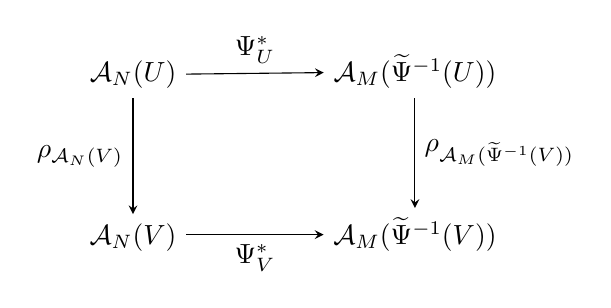
\begin{tikzpicture}
		      		\matrix (m) [matrix of math nodes,row sep=4em,column sep=5em,minimum width=2em]
		      		{
		      			\mathcal{A}_N (U) & \mathcal{A}_M (\widetilde{\Psi}^{-1} (U)) \\
		      			\mathcal{A}_N (V) & \mathcal{A}_M (\widetilde{\Psi}^{-1} (V)) \\
		      		};
		      		\path[-stealth]
		      		(m-1-1) edge node [left] {$\rho_{\mathcal{A}_N (V)}$} (m-2-1)
		      		edge node [above] {$\Psi^*_U$} (m-1-2)
		      		(m-2-1.east|-m-2-2) edge node [below] {$\Psi^*_V$} (m-2-2)
		      		(m-1-2) edge node [right] {$\rho_{\mathcal{A}_M (\widetilde{\Psi}^{-1} (V))}$} (m-2-2);
		      	\end{tikzpicture}
		      \end{center}
		\item Dla dowolnych parzystych współrzędnych $\{ y^1, \ldots, y^{n_0} \}$ na $U \subset N$ zachodzi równość
		      \begin{equation}
		      	\label{eq:psi_psistar}
		      	\widetilde{\Psi^{-1}}^* \circ \varepsilon_\mathcal{N} (y^i) = \varepsilon_\mathcal{M} \circ \Psi_U ^* (y^i), \quad \forall i \in \overline{1, n_0}.
		      \end{equation}
	\end{enumerate}
	Parę $\Psi := ( \widetilde{\Psi}, \Psi^* )$ nazywamy \index{homomorfizm! superrozmaito\'sci}\textit{homomorfizmem superrozmaitości}, co w skrócie zapisujemy $$\Psi: \mathcal{M} \rightarrow \mathcal{N}.$$
\end{definition} 
		      			
\begin{example}
	Rozważmy superrozmaitości $(M, C^\infty_M(\cdot, \mathbb{K}))$ oraz $(N, C^\infty_N(\cdot, \mathbb{K}))$. Każdy dyfeomorfizm $\widetilde{\Phi}: M \rightarrow N$ zadaje homomorfizm superrozmaitości $\Phi = (\widetilde{\Phi}, \Phi^*)$ gdzie $\Phi^*$ jest cofnięciem postaci $\Phi^*(f) = f \circ \widetilde{\Phi}$ dla $f \in C^\infty(U, \mathbb{K})$.
\end{example}
		      			
\begin{remark}
	Warto zauważyć, że z punktu (3) Definicji \ref{def:supermanifold_homomorphism} wynika, że odwzorowanie $\widetilde{\Psi}$ można określić za pomocą $\Psi^*$. Biorąc za parzyste współrzędne $y^i$ lokalne współrzędne rozmaitości $N$ otrzymamy $\varepsilon_\mathcal{N} (y^i) = y^i$ i równanie (\ref{eq:psi_psistar}) sprowadza się do
	\begin{equation*}
		\widetilde{\Psi^{-1}}^* (y^i) = \varepsilon_\mathcal{M} \circ \Psi_U ^* (y^i), \quad \forall i \in \overline{1, n_0},
	\end{equation*}
	co daje obrazy współrzędnych rozmaitości $N$ w odwzorowaniu $\widetilde{\Psi^{-1}}$, które na mocy definicji \ref{def:supermanifold_homomorphism} posiada gładką funkcję odwrotną.
\end{remark}
		      			
Zwróćmy uwagę, że jeśli $M = N$ i odwzorowanie $\widetilde{\Psi}$ jest identycznością na $M$, to $\Psi^*$ w Definicji \ref{def:supermanifold} jest transformacją naturalną snopów $\mathcal{A}_M$ i $\mathcal{A}_N$.
		      			
\begin{definition}
	\label{def:supermanifold_isomomorphism}
	Niech $\Psi := ( \widetilde{\Psi}, \Psi^* )$ będzie homomorfizmem superrozmaitości $\mathcal{M}_1 := (M_1, \mathcal{A}_1)$ oraz $\mathcal{M}_2 := (M_2, \mathcal{A}_2)$. Powiemy, że $\Psi$ jest \index{superrozmaito\'s\'c!izomorpfizm}\textit{izomorfizmem superrozmaitości}, jeśli $\widetilde{\Psi}$ jest dyfeomorfizmem oraz dla każdego otwartego $U \subset M_2$ odwzorowanie $\Psi^*_U$ jest izomorfizmem superalgebr $\mathcal{A}_2(U)$ i $\mathcal{A}_1(\widetilde{\Psi}^{-1}(U))$.
\end{definition}
		      			
Ważnym wynikiem supergeometrii jest twierdzenie Batchelory-Gawędzkiego które pomaga zrozumieć strukturę superrozmaitości \cite{batchelor}.
		      			
\begin{theorem}
	\label{thm:batchelor}
	(Batchelory-Gawędzkiego) Niech $\mathcal{M} := (M, \mathcal A _M)$ będzie rzeczywistą superrozmaitością superwymiaru $(m,n)$. Wtedy istnieją wiązka wektorowa $E \stackrel{\pi}{\rightarrow} M$ rzędu $n$, snop jej cięć $\Gamma_{\Lambda E}$ oraz izomorfizm superrozmaitości $\mu: (M, \Gamma_{\Lambda E}) \rightarrow \mathcal{M}$.
\end{theorem}
		      			
Dla superrozmaitości zespolonych powyższe twierdzenie ma tylko charakter lokalny, ponieważ wymaga rozkładu jedności, który w ogólności nie istnieje na rozmaitościach zespolonych.
		      			
\begin{definition}
	Superrozmaitość $(M, \Gamma_{\Lambda E})$ z Twierdzenia \ref{thm:batchelor} nazywamy \index{superrozmaito\'s\'c!strukturalna}\textit{superrozmaitością strukturalną} superrozmaitości $\mathcal{M}$.
\end{definition}
		      			
Wiązka wektorowa $E$ jest określona z dokładnością do izomorfizmu wiązek wektorowych a izomorfizm superrozmaitości $\mu$ zwykle nie jest izomorfizmem wiązek wektorowych i nie jest kanoniczny. Kategoria superrozmaitości i kategoria wiązek wektorowych nie są izomorficzne.
		      			
Dzięki Twierdzeniu Batchelory-Gawędzkiego wiemy, że każda superrozmaitość ma swoją superrozmaitość strukturalną i na niej można by zdefiniować superwspółrzędne. Jednak do obliczeń praktycznych warto zdefiniować superukład współrzędnych jak najogólniej.
		      			
\section{Superrozmaitość styczna}
		      			
W supermechanice pojawią się superrównania Eulera-Lagrange'a \cite{carinena}. Do ich wprowadzenia potrzebne będą pojęcia superrozmaitości stycznej i superpól wektorowych. Niech $\mathcal{M} := (M, \mathcal{A}_M)$ będzie superrozmaitością o superwymiarze $(m,n)$. Pokażemy jak z jej pomocą skonstruować nową superrozmaitość $\mathcal{T} \mathcal{M} := (TM, \mathcal{A}_{TM})$, która jest uogólnieniem wiązki stycznej do $M$.
		      			
Do zdefiniowania superrozmaitości stycznej potrzeba definicji snopa $\mathcal{A}_{TM}$. Każdemu $TU$ dla otwartegu $U \subset M$ przyporządkujmy $\mathcal{A}_{TM}(TU) := C^\infty (TU) \otimes \Lambda \mathbb{K}^{2n}$ oraz każdemu morfizmowi inkluzji $TV \subset TU$ przyporządkujmy morfizm restrykcji $\rho_{TU,TV}: \mathcal{A}_{TM}(TU) \ni f \mapsto f|_{V} \in \mathcal{A}_{TM}(TV)$. Tak określony $\mathcal{A}_{TM}$ jest presnopem.
		      			
Żeby zagwarantować, że $\mathcal{A}_{TM}$ jest snopem, musimy odpowiednio zdefiniować tranformacje współrzędnych na przecięciach otwartych podzbiorów $TM$. 
		      			
Z Twierdzenia \ref{thm:batchelor} wynika istnienie superrozmaitości strukturalnej $(M, \Gamma_{\Lambda E})$ superrozmaitości $\mathcal{M}$ oraz istnienie rodziny superwspółrzędnych, które transformują się jak współrzędne na wiązce wektorowej $E \stackrel{\pi}{\rightarrow} M$. Stąd na otwartych $U_\alpha, U_\beta \subset M$ istnieją superwspółrzędne $\{a^i, \theta^\mu \}^{\mu \in \overline{1,n}} _{i \in \overline{1,m}}$ oraz $\{b^i, \xi^\mu \}^{\mu \in \overline{1,n}} _{i \in \overline{1,m}}$ takie, że na $U_\alpha \cap U_\beta$ transformacja współrzędnych jest postaci
\begin{equation}
	\label{eq:supercoords}
	b^i = \varphi^i(a^1, \ldots, a^m), \quad i \in \overline{1,m}, \qquad
	\xi^\mu = \psi_\nu^\mu(a_1, \ldots, a_m) \theta^\nu, \quad \mu \in \overline{1,n},
\end{equation}
dla pewnych  funkcji $\varphi^i$ oraz $\psi^\mu _\nu$. W superalgebrach $\mathcal{A}_{TM}(TU_\alpha), \mathcal{A}_{TM}(TU_\beta)$ wybieramy generatory $\{a^i, \dot{a}^i, \theta^\mu, \dot{\theta}^\mu \}^{\mu \in \overline{1,n}} _{i \in \overline{1,m}}$ oraz $\{b^i, \dot{b}^i, \xi^\mu, \dot{\xi}^\mu \}^{\mu \in \overline{1,n}} _{i \in \overline{1,m}}$, w których 
\begin{itemize}
	\item $a^i, b^i, \theta^\mu, \xi^\mu$ są superwspółrzędnymi transformującymi się jak w (\ref{eq:supercoords}),
	\item $\dot{a}^i, \dot{b}^i$ są współrzędnymi indukowanymi przez $a^i, b^i$ na wiązce stycznej $TM$,
	\item $\dot{\theta}^\mu, \dot{\xi}^\mu$ są generatorami nieparzystymi takimi, że$$ \{ a^i, \dot{a}^i, \theta^\mu, \dot{\theta}^\mu \}^{\mu \in \overline{1,n}} _{i \in \overline{1,m}},\qquad \{ b^i, \dot{b}^i, \xi^\mu, \dot{\xi}^\mu \}^{\mu \in \overline{1,n}} _{i \in \overline{1,m}}$$ spełniają, że $\mathcal{A}_{TM}(TU_\alpha)\simeq C^\infty(U_\alpha) \otimes \Lambda \mathbb{K}^n$ oraz $\mathcal{A}_{TM}(TU_\beta) \simeq C^\infty(U_\beta)\otimes \Lambda \mathbb{K}^n$.
\end{itemize}
Transformację superwspółrzędnych (izomorfizm superalgebr) na $TU_\alpha \cap TU_\beta$ definiujemy dodając do reguł (\ref{eq:supercoords}) zależności, które odpowiadają różniczkowaniom funkcji przejścia przestrzeni konfiguracyjnej:
\begin{equation}
	\begin{gathered}
		\dot{b}^i = \frac{\partial \varphi^i (a^1, \ldots, a^m)}{\partial a^j} \dot{a}^j, \quad i \in \overline{1,m}, \\
		\dot{\xi}^\mu = \frac{\partial \psi^\mu_\nu(a^1, \ldots, a^m)}{\partial a^j} \dot{a}^j \theta^\nu + \psi^\mu_\nu(a^1, \ldots, a^m) \dot{\theta}^\nu, \quad \mu \in \overline{1,n}.
	\end{gathered}
\end{equation}
		      			
Pokażemy, że tak zdefiniowane transformacje superwspółrzędnych superrozmaitości stycznej spełniają warunek kocyklu. Niech otwarte zbiory $U_1, U_2, U_3 \subset M$ mają niepuste przecięcie. Wybierzmy superukład współrzędnych $(x^i, \theta^\mu)$ na $U_1$, superukład $(y^i, \xi^\mu)$ na $U_2$ oraz superukład $(z^i, \eta^\mu)$ na $U_3$. Niech $\varphi_{12},\varphi_{23},\varphi_{31}$ będą transformacjami superwspółrzędnych parzystych, a $\psi, \chi, \phi$ będą transformacjami superwspółrzędnych nieparzystych, odpowiednio z $U_1$ do $U_2$, z $U_2$ do $U_3$ i z $U_3$ do $U_1$. Opisaną sytuację przedstawiono na Rysunku \ref{fig:supertangent_coord}.
		      			
\begin{figure}[htb]
	\centering
	\includegraphics[width=0.5\textwidth]{supertangent_coord.pdf}
	\caption{Ilustracja zbiorów $U_1, U_2, U_3$ i zmiany superwspółrzędnych między nimi.}
	\label{fig:supertangent_coord}
\end{figure}
		      			
Fakt, że transformacje superwspółrzędnych $\{ x^i, \dot{x}^i, \theta^\mu \}$ spełniają warunki kocyklu
\begin{equation*}
	\varphi_{12}^i \varphi_{23}^i \varphi_{31}^i = \I, \quad \frac{\partial \varphi^k_{31}}{\partial z^n} \frac{\partial \varphi^n_{23}}{\partial y^m} \frac{\partial \varphi^k_{12}}{\partial x^l} = \delta^k _l, \quad \phi ^\alpha _\beta \chi ^\beta _\gamma \psi ^\gamma _\mu = \delta ^\alpha _\mu
\end{equation*}
wynika z własności wiązki stycznej $TM$ i własności wiązki wektorowej $E \stackrel{\pi}{\rightarrow} M$. 
Dla superwspółrzędnych $\{ \dot{\theta}^\mu \}$ udowadniamy to licząc złożenie $\Phi$ trzech transformacji superwspółrzędnych nieparzystych w postaci macierzowej (\ref{eq:supercoord_matrix}).
\begin{equation}
	\label{eq:supercoord_matrix}
	\Phi :=
	\left[ \begin{array}{cc}
		\phi ^\alpha _\beta & 0 \\
	\frac{\partial \phi ^\alpha _\beta}{\partial z^i}\dot z^i & \phi ^\alpha _\beta \end{array} \right]
	\left[ \begin{array}{cc}
		\chi ^\beta _\gamma & 0 \\
	\frac{\partial \chi ^\beta _\gamma}{\partial y^j}\dot y^j & \chi ^\beta _\gamma \end{array} \right]
	\left[ \begin{array}{cc}
		\psi ^\gamma _\alpha & 0 \\
	\frac{\partial \psi ^\gamma _\alpha}{\partial x^k}\dot x^k & \psi ^\gamma _\alpha \end{array} \right]
	=
	\left[ \begin{array}{cc}
		\phi ^\alpha _\beta \chi ^\beta _\gamma \psi ^\gamma _\alpha & 0 \\
		M & \phi ^\alpha _\beta \chi ^\beta _\gamma \psi ^\gamma _\alpha
	\end{array} \right]\!,
\end{equation}
gdzie macierz $M$ ma postać:
\begin{equation*}
	M = \frac{\partial \phi ^\alpha _\beta}{\partial z^i} \chi ^\beta _\gamma \psi ^\gamma _\alpha \dot z^i + \phi ^\alpha _\beta \frac{\partial \chi ^\beta _\gamma}{\partial y^j} \psi ^\gamma _\alpha \dot y^j + \phi ^\alpha _\beta \chi ^\beta _\gamma \frac{\partial \psi ^\gamma _\alpha}{\partial x^k}\dot x^k.
\end{equation*}
Zauważmy, że 
$$\frac{\partial \phi ^\alpha _\beta}{\partial z^i}\dot z^i = \frac{\partial \phi ^\alpha _\beta}{\partial x^m} \frac{\partial x^m}{\partial z^i} \frac{\partial \dot z^i}{\partial \dot x^k} \dot x^k = \frac{\partial \phi ^\alpha _\beta}{\partial x^k} \dot x^k.$$
Podobnie $\frac{\partial \chi ^\beta _\gamma}{\partial y^j}\dot y^j = \frac{\partial \chi ^\beta _\gamma}{\partial x^k}\dot x^k$, a zatem 
\begin{equation*}
	M = \frac{\partial}{\partial x^k} \left( \phi ^\alpha _\beta \chi ^\beta _\gamma \psi ^\gamma _\alpha \right) \dot x^k = 0
\end{equation*}
co oznacza, że $\Phi = \I_{2n\times 2n}$ i ostatni warunek kocyklu też jest spełniony. Zachodzenie warunków kocyklu gwarantuje, że spełnione jest poniższe
		      			
\begin{theorem}
	\label{thm:supertangent_sheaf01}
	$\mathcal{A}_{\mathcal{TM}}$ jest snopem.
\end{theorem}
		      			
Snopem elementów nilpotentnych $\mathcal{N}_{TM}$ snopu $\mathcal{A}_{TM}$ jest snop superalgebr lokalnie generowanych przez współrzędne nieparzyste. Skoro $\mathcal{A}_{M}/\mathcal{N}_M\simeq C^\infty(\cdot,M)$ z założenia, to można udowodnić, że $\mathcal{A}_{TM} / \mathcal{N}_{TM} \simeq C^\infty(\cdot,{TM})$. Wobec tego $\mathcal{T} \mathcal{M} := (TM, \mathcal{A}_{TM})$ jest superrozmaitością.
		      			
\begin{definition}
	Superrozmaitość $\mathcal{T} \mathcal{M}: = (TM, \mathcal{A}_{TM})$ skonstruowaną powyżej nazywamy \index{superwi\k azka styczna}\textit{superwiązką styczną} do superrozmaitości $\mathcal{M} := (M, \mathcal{A}_M)$, zaś $\mathcal{A}_{TM}$ nazywamy \index{supersnop styczny}\textit{supersnopem stycznym} snopa $\mathcal{A}_{M}$.
\end{definition}
		      			
\begin{proposition}
	Jeśli $E \stackrel{\pi}{\rightarrow} M$ jest wiązką strukturalną superrozmaitości $\mathcal{M} = (M, \mathcal{A}_M)$, to wiązka $TE \stackrel{T\pi}{\longrightarrow} TM$ jest wiązką strukturalną superrozmaitości stycznej $\mathcal{T} \mathcal{M}$.
\end{proposition}
		      			
\subsection{Superpola wektorowe}
		      			
Skoro dla każdego otwartego $U \subset M$ mamy supermoduł $\mathrm{Der}(\mathcal{A}_\mathcal{M}(U))$, możemy zdefiniować snop supermodułów superróżniczkowań $\mathcal{A'}_{\mathcal{M}}$ tak, że
\begin{equation}
	\begin{gathered}
		U \mapsto \mathrm{Der}(\mathcal{A}_\mathcal{M}(U)), \qquad \forall \ \mathrm{otwartego}\ U \subset M, \\
		\rho_{VU} \mapsto \rho'_{VU}, \qquad \forall \ \mathrm{otwartego}\ V, U, \ \mathrm{gdzie\ } V \subset U \subset M,
	\end{gathered}
\end{equation}
przy czym przez $\rho_{VU}$ rozumiemy obcięcie z $U$ do $V$, zaś $\rho'_{VU}$ jest odwzorowaniem
\begin{equation}
	\begin{array}{rccc}
		\rho'_{VU}: & {\rm Der}(\mathcal{A}_M(U)) & \rightarrow & {\rm Der}(\mathcal{A}_M(V)) \\
		            & D                           & \mapsto     & \rho'_{UV}(D)               
	\end{array}
\end{equation} \\[-13pt]
dla
\begin{equation*}
	\begin{aligned}
		\rho'_{VU}(D) \rho_{VU}(f) := \rho_{VU}(Df),                                      
		\qquad \forall D\in {\rm Der}(\mathcal{A}_M(U)),\; \forall f\in \mathcal{A}_M(U). 
	\end{aligned}
\end{equation*}
		      			
\begin{definition}
	Cięcia snopa $\mathcal{A'_{M}}$ nazywamy \index{superpole wektorowe}\textit{superpolami wektorowymi} na superrozmaitości $\mathcal{M}$. 
\end{definition}
		      			
Zbiór superpól wektorowych nad superrozmaitością $\mathcal M$ oznaczamy $\mathfrak{X}(\mathcal{M})$. Inaczej niż w geometrii różniczkowej, w supergeometrii superpola wektorowe na $\mathcal{M}$ nie są cięciami snopa superrozmaitości stycznej, tylko cięciami tzw. superwiązki stycznej \cite{carinena}. Z drugiej strony widać, że superrozmaitość styczna w ogólności nie jest superwiązką nad superrozmaitością pierwotną, ponieważ rzutowanie $\mathcal{A_{TM}} \rightarrow \mathcal{A_M}$ może nie istnieć.
		      			
Podobnie jak w geometrii różniczkowej, można pokazać \cite{rogers}, że superpole wektorowe $X$ w lokalnych superwspółrzędnych $(x^i, \theta^\mu)$ przyjmuje postać \\[-5pt]
\begin{equation*}
	X = X^{x^i} \frac{\partial}{\partial x^i} + X^{\theta^\mu} \frac{\partial}{\partial \theta^\mu},
\end{equation*}
gdzie $X^{x^i}, X^{\theta^\mu}$ są superfunkcjami na $\mathcal{M}$. Widać, że dla superwymiaru $(m,n)$ superrozmaitości $\mathcal{M}$ zachodzi $\mathcal{A'_{TM}} \simeq \mathcal{A_{TM}}^{2m+2n}$.
		      			
\begin{example} 
	Rozważmy transformację superwspółrzędnych $(x, \theta) \mapsto (y, \Upsilon)$ na $\mathbb{R}^{1|1}$ taką, że
	\begin{equation}
		\label{eq:superfield_transformation_coords01}
		y:= \log (x), \quad \Upsilon := (1+x^2) \theta.
	\end{equation}
	Relacje (\ref{eq:superfield_transformation_coords01}) indukują transformację $\dot x, \dot \theta$ na superrozmaitości stycznej $\mathcal{T} \mathbb{R}^{1|1}$ w postaci 
	\begin{equation}
		\label{eq:superfield_transformation_coords02}
		\dot y=\dot x/x,\quad \dot \Upsilon=2x\dot x\theta+(1+x^2)\dot \theta.
	\end{equation}
	Zbadajmy, jak zmienia się zapis superpola wektorowego $X \in \mathfrak{X}(\mathcal{T} \mathbb{R}^{1|1})$ zadanego wzorem
	\begin{equation}
		\label{eq:the_x_equation}
		X=\dot x\frac{\partial}{\partial x}-x\frac{\partial}{\partial \dot x}+\dot\theta\frac{\partial}{\partial \theta}-\theta\frac{\partial}{\partial \theta}
	\end{equation}
	pod wpływem zamiany zmiennych $(x, \dot x, \theta, \dot \theta) \mapsto (y, \dot y, \Upsilon, \dot \Upsilon)$ na $\mathcal{T}\mathbb{R}^{1|1}$. W nowych zmiennych $X$ przyjmuje ogólną postać
	\begin{equation*}
		X=(Xy)\frac{\partial}{\partial y}+(X\dot y)\frac{\partial}{\partial \dot y}+(X\Upsilon)\frac{\partial}{\partial \Upsilon}+(X\dot \Upsilon)\frac{\partial}{\partial \dot\Upsilon}.
	\end{equation*}
	Ponieważ
	\begin{equation*}
		\begin{gathered}
			Xy=X\log x=\frac{\dot x}{x}=\dot y,\quad X\dot y=X\frac{\dot x}{x}=-\frac{\dot x^2}{x^2}-1=-\dot y^2-1 \\
			X\Upsilon=2x\dot x\theta+(1+x^2)\dot\theta =\dot \Upsilon, \quad X\dot\Upsilon=\frac{4e^{2y}\dot y}{1+e^{2y}}\dot\Upsilon +\frac{\Upsilon}{(1+e^{2y})^2}[6e^{4y}(6\dot y^2-3)-4e^{2y}-1],
		\end{gathered}
	\end{equation*}
	otrzymujemy
	\begin{equation*}
		X=\dot y\frac{\partial}{\partial y}-(\dot y^2+1)\frac{\partial }{\partial \dot y}+\dot\Upsilon\frac{\partial}{\partial \Upsilon}+\left[\frac{4e^{2y}\dot y}{1+e^{2y}}\dot\Upsilon +\frac{\Upsilon}{(1+e^{2y})^2}[6e^{4y}(6\dot y^2-3)-4e^{2y}-1]\right]\frac{\partial}{\partial \dot\Upsilon}.
	\end{equation*}
\end{example}
		      			
W ogólnym przypadku superpola wektorowego $X \in \mathfrak{X}(\mathcal{M})$ postaci (\ref{eq:the_x_equation}) dla superwspółrzędnych lokalnych $x^i, \theta^\mu$ na pewnej superrozmaitości $\mathcal{M}$, superwspółrzędne $\dot x^i, \dot \theta^\mu$ można traktować jak odwzorowania spełniające relacje
\begin{equation*}
	\dot \theta^\alpha(X)=X\theta^\alpha,\quad \dot x^i(X)=X x^i.
\end{equation*}
		      			
\begin{proposition}
	Niech $D \in \mathfrak{X}(\mathcal{M})$ i niech $\widetilde{D}$ będzie postaci
	\begin{equation*}
		\widetilde{D}\widetilde{f}:=\widetilde{Df},\qquad \forall f\in \mathcal{A}_M,
	\end{equation*}
	gdzie $\widetilde f=\varepsilon(f)$ dla morfizmu $\varepsilon:\mathcal{A}_\mathcal{M} \rightarrow \mathcal{A}_\mathcal{M}/\mathcal{F}_\mathcal{M}\simeq C^\infty(M)$. Wtedy $\widetilde{D}$ jest polem wektorowym na $M$. \cite{monterde}
\end{proposition}
		      			
\begin{example}
	Cząstkę klasyczną nierelatywistyczną można opisać superpolem wektorowym $\Gamma \in \mathfrak{X}(\mathcal{T} \mathbb{C}^{3|3})$ (patrz Przykład \ref{ex:superfield}) postaci
	\begin{equation*}
		\Gamma = \dot q^i \frac{\partial}{\partial q^i} 
		- \frac{1}{m} \left( \frac{\partial V}{\partial q^i} + \frac{\partial V_{\mu \nu}}{\partial q^i} \theta^\mu \theta^\nu \right) \frac{\partial}{\partial \dot q^i} 
		- 2{\rm i} \theta^\nu V_{\mu \nu} \frac{\partial}{\partial \theta^\mu}.
	\end{equation*}
	Weźmy dowolną superfunkcję $f \in C^\infty(\mathcal{\mathcal{T}} \mathbb{C}^{3|3})$ o ogólnej postaci \\[-7pt]
	\begin{equation*}
		\begin{gathered}
			f(q,\dot q, \theta, \dot \theta) := \!\!\!\!\!\!\!\!
			\sum_{\underline{\lambda} \in \mathfrak{M}^3,\; \underline{\alpha} \in \mathfrak{M}^3} \!\!\!\!\!\!\!\! f^{\theta^{\left[\, \underline{\lambda}\, \right]} \dot \theta^{\left[\, \underline{\alpha}\, \right]}} (q, \dot q) \theta^{\left[\, \underline{\lambda}\, \right]} \dot \theta^{\left[\, \underline{\alpha}\, \right]}.
		\end{gathered}
	\end{equation*}\\[-13pt]
	Skoro $\widetilde \Gamma \widetilde f = \widetilde{\Gamma f}$, to\\[-7pt]
	\begin{equation*}
		\widetilde \Gamma \widetilde f = \dot q^i\frac{\partial f^0}{\partial q^i}
		-\frac1m \frac{\partial V}{\partial q^i}\frac{\partial f^0}{\partial \dot q^i} \quad 
		\Longrightarrow \quad \widetilde \Gamma = \dot q^i\frac{\partial}{\partial q^i} - \frac1m \frac{\partial V}{\partial q^i}\frac{\partial}{\partial \dot q^i}.
	\end{equation*}
\end{example}
		      			
Pokażemy teraz sposób całkowania superpól wektorowych parzystych. Przypominamy, że w geometrii różniczkowej układ równań różniczkowych na krzywą całkową $\gamma_x (t) = (\gamma_x ^1(t), \ldots, \gamma_x ^m (t))$ pola wektorowego $X$ na rozmaitości $M$ wymiaru $m$ ma postać
\begin{equation}
	\label{eq:flow_system}
	\frac{d}{dt}\gamma_{x}^i(t)=X^i(\gamma_{x}(t)), \quad i \in \overline{1,m},
\end{equation}
gdzie $\gamma_{x}$ to rozwiązanie szczególne układu (\ref{eq:flow_system}) z warunkiem początkowym $\gamma_x(0) = x \in M.$ Definiuje się potok pola $X$ jako odwzorowanie $\gamma(\cdot, \cdot): \mathbb{R} \times M \rightarrow M$ takie, że $\gamma(t, x) := \gamma_x (t).$ Dla pola wektorowego $X$ można również zdefiniować funkcję $\Gamma^* : C^\infty (M) \rightarrow C^\infty (\mathbb{R} \times M)$ za pomocą warunków
\begin{equation*}
	\Gamma^*(x^i) := x^i(\gamma(\cdot, \cdot)) =  \gamma^i(\cdot, \cdot), \quad i \in \overline{1,m},
\end{equation*}
gdzie przez $x^i$ rozumiemy funkcję współrzędnościową zwracającą $i$-tą współrzędną punktu $x\in M$ w ustalonych lokalnych współrzędnych $M$. Wtedy
\begin{equation}
	\label{eq:flow_general}
	\frac{\partial \Gamma^*(x^i)}{\partial t}(t, x) 
	= \frac{d}{dt} \gamma^i_x(t) = X^i(\gamma_x(t)) = X^i(\gamma(t,x))=\Gamma^*(Xx^i) (t,x). 
\end{equation}
Skoro równość (\ref{eq:flow_general}) jest spełniona dla wszystkich funkcji współrzędnościowych $x^i$, to można pokazać, że $D\circ \Gamma^*=\Gamma^*\circ X$, gdzie $D = \frac{\partial}{\partial t}$, zachodzi dla dowolnej funkcji $f \in C^\infty(M)$. W supergeometrii korzysta się z uogólnienia tego równania do zdefiniowania potoku superpola wektorowego.
		      			 
\begin{definition}
	\index{superpotok}\textit{Superpotokiem superpola wektorowego} $X \in \mathfrak{X}(\mathcal{M})$ nazywamy homomorfizm superrozmaitości $\Gamma : \mathbb{R} \times \mathcal{M} \rightarrow \mathcal{M}$ taki, że $\widetilde \Gamma$ to potok $\mathbb{R} \times M \rightarrow M$ pola wektorowego $\widetilde X$, natomiast $\Gamma^*$ spełnia relację
	\begin{equation*}
		D\circ \Gamma^*=\Gamma^*\circ X
	\end{equation*}
	oraz warunek $\Gamma^*_{M} (f )(0,x) = f(x)$ dla dowolnej funkcji $f \in C^\infty (M)$ i dowolnego $x \in M.$
\end{definition}
		      			 
\begin{example}
	Zbadamy klasyczny jednowymiarowy superoscylator harmoniczny \cite{So99}. Można pokazać, że superpole wektorowe $X \in \mathfrak{X}(\mathcal{T}\mathbb{R}^{1|1})$ o lokalnej postaci
	\begin{equation*}
		X = \dot x \frac{\partial}{\partial x} - x \frac{\partial}{\partial \dot x} + \dot \theta \frac{\partial}{\partial \theta} - \theta \frac{\partial}{\partial \dot \theta}
	\end{equation*}
	jest rozwiązaniem superrównania Eulera-Lagrange'a (\ref{eq:sele}) dla superlagranżjanu superoscylatora harmonicznego w superwymiarze $(1,1)$. Dynamikę takiego układu opisuje superpotok $\Gamma: \mathbb{R} \times \mathcal{T} \mathbb{R}^{1|1} \rightarrow \mathcal{T} \mathbb{R}^{1|1}$ superpola wektorowego $X$. W tym przykładzie pokażemy, jak go znaleźć, czyli jak określić $\Gamma^*$ i $\widetilde{\Gamma}$.
					      				
	Wykorzystując globalne superwspółrzędne $(x, \dot x, \theta, \dot \theta)$ na $\mathcal{T} \mathbb{R}^{1|1}$ i fakt, że dla każdego otwartego $U\subset \mathbb{R}^{1|1}$ odwzorowanie $\Gamma^*_U$ jest parzystym homomorfizmem superalgebr otrzymujemy równania na obrazy funkcji współrzędnościowych na $\mathcal{T} \mathbb{R}^{1|1}$
	\begin{equation}
		\label{eq:superharmonic_superflow_star}
		\begin{gathered}
			\Gamma_U^*(x) (t,x,\dot x) =\Gamma^x(t,x,\dot x)+\Gamma^x_{\theta\dot\theta}(t,x,\dot x)\theta\dot\theta,\qquad 
			\Gamma_U^*(\dot x) (t,x,\dot x) =\Gamma^{\dot x}(t,x,\dot x)+\Gamma^{\dot x}_{\theta\dot\theta}(t,x,\dot x)\theta\dot\theta, \\
			\Gamma_U^*(\theta) (t,x,\dot x) =\Gamma^\theta_\theta(t,x,\dot x) \theta+\Gamma^\theta_{\dot\theta}(t,x,\dot x) \dot \theta,\qquad
			\Gamma_U^*(\dot\theta) (t,x,\dot x) =\Gamma^{\dot \theta}_\theta(t,x,\dot x) \theta+\Gamma^{\dot \theta}_{\dot\theta}(t,x,\dot x) \dot \theta,
		\end{gathered}
	\end{equation}
	gdzie $\Gamma^\alpha_\beta (t,x,\dot x) \in C^\infty (\mathbb{R}\times T \mathbb{R})$ dla dowolnych indeksów $\alpha, \beta \in \{ - ,x, \dot x, \theta, \dot \theta, \theta \dot \theta \}$. Na podstawie układu równań (\ref{eq:superharmonic_superflow_star}) można określić obraz dowolnej funkcji $f \in C^\infty(\mathcal{T} \mathbb{R}^{1|1})$: przypuśćmy, że $$f(x, \dot x, \theta, \dot \theta)\ = \!\!\!\!\!\!\!\!
	\sum_{\underline{\lambda} \in \mathfrak{M}^3,\; \underline{\alpha} \in \mathfrak{M}^3} \!\!\!\!\!\!\!\! f^{\theta^{\left[\, \underline{\lambda}\, \right]} \dot \theta^{\left[\, \underline{\alpha}\, \right]}} (x, \dot x) \theta^{\left[\, \underline{\lambda}\, \right]} \dot \theta^{\left[\, \underline{\alpha}\, \right]},$$
	a wtedy z własności homomorfizmu superalgebr otrzymamy
	\begin{equation*}
		\Gamma_U^* (f) (t,x, \dot x)\ = \!\!\!\!\!\!\!\!
		\sum_{\underline{\lambda} \in \mathfrak{M}^3,\; \underline{\alpha} \in \mathfrak{M}^3} \!\!\!\!\!\!\!\! f^{\theta^{\left[\, \underline{\lambda}\, \right]} \dot \theta^{\left[\, \underline{\alpha}\, \right]}} (\Gamma^*_U x, \Gamma^*_U \dot x) \Gamma^*_U \theta^{\left[\, \underline{\lambda}\, \right]} \Gamma^*_U \dot \theta^{\left[\, \underline{\alpha}\, \right]}.
	\end{equation*}
	Jeśli równanie $D \circ \Gamma^* = \Gamma^* \circ X$ jest spełnione dla globalnych funkcji współrzędnościowych $x, \dot x, \theta, \dot \theta$, to z liniowości $D, \Gamma^*$ oraz $X$ jest ono spełnione dla dowolnej superfunkcji $f \in C^\infty (\mathcal{T} \mathbb{R}^{1|1})$. W szczególności \\[-7pt]
	\begin{equation*}
		\begin{gathered}
			D\circ\Gamma^*(x)=\Gamma^*\circ Xx\quad \Longrightarrow\quad D\Gamma^x+D\Gamma^x_{\theta\dot\theta}\theta\dot\theta =\Gamma^{\dot x}+\Gamma^{\dot x}_{\theta\dot\theta}\theta\dot\theta\quad \Longrightarrow\quad \left\{ \begin{array}{l}
			D\Gamma^x=\Gamma^{\dot x}, \\
			D\Gamma_{\theta\dot\theta}^x=\Gamma_{\theta\dot\theta}^{\dot x}, \end{array} \right. \\
			D\circ \Gamma^*(\dot x) =\Gamma^*\circ X\dot x\quad \Longrightarrow\quad D\Gamma^{\dot x}+D\Gamma^{\dot x}_{\theta\dot\theta}\theta\dot\theta =-\Gamma^{x}-\Gamma^{x}_{\theta\dot\theta} \theta \dot \theta \quad \Longrightarrow\quad \left\{ \begin{array}{l}
			D\Gamma^{\dot x}=-\Gamma^{x}, \\
			D\Gamma_{\theta\dot\theta}^{\dot x} = -\Gamma_{\theta \dot \theta}^{x}, \end{array} \right. \\
			D\circ \Gamma^*(\theta)=\Gamma^*\circ X\theta\quad \Longrightarrow\quad  D\Gamma^\theta_\theta\theta+D\Gamma^\theta_{\dot\theta}\dot\theta =\Gamma^{\dot \theta}_{\theta}\theta+\Gamma^{\dot \theta}_{\dot\theta}\dot \theta\quad \Longrightarrow\quad \left\{ \begin{array}{l}
			D\Gamma^\theta_\theta=\Gamma^{\dot\theta}_\theta, \\
			D\Gamma^\theta_{\dot\theta}=\Gamma^{\theta}_{\dot\theta}, \end{array} \right. \\
			D\circ \Gamma^*(\dot \theta)=\Gamma^*\circ X\dot \theta\quad \Longrightarrow\quad D\Gamma^{\dot \theta}_\theta\theta+D\Gamma^{\dot \theta}_{\dot\theta}\dot \theta=-\Gamma^{\theta}_\theta\theta-\Gamma^{\theta}_{\dot\theta}\dot\theta\quad \Longrightarrow\quad \left\{ \begin{array}{l}
			D\Gamma^{\dot \theta}_\theta=-\Gamma^{\theta}_\theta, \\
			D\Gamma^{\dot\theta}_{\dot \theta}=-\Gamma_{\dot\theta}^{\theta}. \end{array} \right.
		\end{gathered}
	\end{equation*}
	Stąd wynika, że
	\begin{equation}
		\label{eq:superflow_coeff_conditions}
		\begin{gathered}
			D^2\Gamma^x=-\Gamma^x,\quad \Gamma^{\dot x}=D\Gamma^x,\qquad
			D^2\Gamma^\theta_{\theta}=-\Gamma^\theta_{\theta},\quad \Gamma^{\dot\theta}_{\theta}=D\Gamma^{\theta}_{\theta},\\
			D^2\Gamma^{\dot\theta}_{\dot \theta}=-\Gamma^{\dot\theta}_{\dot\theta},\quad \Gamma^{\theta}_{\dot\theta}=-D\Gamma^{\dot\theta}_{\dot\theta},\qquad
			D^2\Gamma^x_{\theta\dot\theta}=-\Gamma^x_{\theta\dot \theta},\quad D\Gamma^{x}_{\theta\dot\theta}=\Gamma^{\dot x}_{\theta\dot\theta}.
		\end{gathered}
	\end{equation}
	Rozwiązując równania (\ref{eq:superflow_coeff_conditions}) dla superróżniczkowania $D = \frac{\partial}{\partial t}$ otrzymujemy
	\begin{equation}
		\begin{gathered}
			\Gamma^x =A(x,\dot x)\cos (t)+\hat A(x,\dot x)\sin(t),\qquad  \Gamma^{\dot x}=-A(x,\dot x)\sin (t)+\hat A(x,\dot x)\cos(t),\\
			\Gamma^\theta_\theta =B(x,\dot x)\cos (t)+\hat B(x,\dot x)\sin(t),\qquad \Gamma^{\dot \theta}_\theta=-B(x,\dot x)\sin (t)+\hat B(x,\dot x)\cos(t),\\
			\Gamma^{\dot \theta}_{\dot \theta} =C(x,\dot x)\cos (t)+\hat C(x,\dot x)\sin(t),\qquad \Gamma^{\theta}_{\dot \theta}=C(x,\dot x)\sin (t)-\hat C(x,\dot x)\cos(t),\\
			\Gamma^x_{\theta\dot\theta} =D(x,\dot x)\cos (t)+\hat D(x,\dot x)\sin(t),\qquad  \Gamma^{\dot x}_{\theta\dot\theta}=-D(x,\dot x)\sin (t)+\hat D(x,\dot x)\cos(t).
		\end{gathered}
	\end{equation}
	Ponieważ dla $t=0$ zachodzą warunki
	\begin{equation*}
		\begin{gathered}
			\Gamma^*(x)=A(x,\dot x)+D(x,\dot x)\theta\dot\theta=x,\qquad\Gamma^*\dot x=\hat A(x,\dot x)+\hat D(x,\dot x)\theta\dot\theta=\dot x,\quad\\
			\Gamma^*(\theta)=B(x,\dot x)\theta-\hat C(x,\dot x)\dot\theta=\theta,\qquad
			\Gamma^*(\dot \theta)=C(x,\dot x)\dot\theta+\hat B(x,\dot x)\theta=\dot\theta,
		\end{gathered}
	\end{equation*}
	muszą być spełnione relacje
	\begin{equation*}
		\begin{gathered}
			A(x,\dot x)=x,\quad \hat A(x,\dot x)=\dot x, \qquad B(x,\dot x)=1, \quad \hat B(x,\dot x)=0, \\ C(x,\dot x)=1, \quad \hat C(x,\dot x)=0, \qquad D(x,\dot x)=0, \quad \hat D(x,\dot x)=0.
		\end{gathered}
	\end{equation*}
	Ostatecznie
	\begin{equation*}
		\begin{gathered}\Gamma^*(x)=x\cos(t)+\dot x\sin(t),\qquad\Gamma^*(\dot x)=-x\sin(t)+\dot x\cos(t),\\
			\Gamma^*(\theta)=\cos(t)\theta+\sin(t)\dot\theta,\qquad
			\Gamma^*(\dot \theta)=\cos(t)\dot\theta-\sin(t)\theta.
		\end{gathered}
	\end{equation*}
					      				
	Do znalezienia pozostał potok $\widetilde \Gamma$ pola wektorowego $\widetilde X$. Pole wektorowe $\widetilde X$ poznamy badając relację $\widetilde X \widetilde f = \widetilde{Xf}$ dla dowolnej $f\in C^\infty(\mathcal{T} \mathbb{R}^{1|1})$ opisanej w superwspółrzędnych wzorem $f(x,\dot x,\theta,\dot\theta)=f^0(x,\dot x)+f^\theta(x,\dot x)\theta+f^{\dot\theta}(x,\dot x)\dot\theta+f^{\theta\dot\theta}(x,\dot x)\theta\dot \theta.
	$
	Widać, że
	\begin{equation*}
		\widetilde{Xf} = \dot x \frac{\partial f^0}{\partial x} - x \frac{\partial f^0}{\partial \dot x} \quad \Longrightarrow \quad \widetilde X = \dot x \frac{\partial}{\partial x} - x \frac{\partial}{\partial \dot x},
	\end{equation*}
	zatem krzywe całkowe $\widetilde{X}$ są rozwiązaniami układu równań różniczkowych postaci
	\begin{equation*}
		\left\{\begin{aligned}
		\frac{dx}{dt}&= \dot x, \\
		\frac{d \dot x}{dt}& = -x,
		\end{aligned}\right.\quad\Longrightarrow\quad \frac{d}{dt}\left[\begin{array}{c}x\\ \dot x \end{array}\right]=\left[\begin{array}{cc}0&1\\-1&0\end{array}\right]\left[\begin{array}{c}x\\ \dot x \end{array}\right]\!.
	\end{equation*}
	Wobec tego krzywe te są określone we współrzędnych poprzez $x(t) = x_0 \cos (t) + v_0 \sin (t), \dot x (t) = v_0 \cos (t) - x_0 \sin (t)$ i potok $\widetilde{\Gamma}$ ma postać
	\begin{equation*}
		\widetilde{\Gamma}: \mathbb{R}\times TM \ni (t,x,\dot x) \mapsto (x \cos(t)+\dot x \sin(t), \dot x \cos(t)- x \sin(t))\in TM.
	\end{equation*}
\end{example}
		      			
Na zakończenie podrozdziału o superpolach wektorowych wspomnimy o superkomutatorze, który jest naturalnym rozszerzeniem komutatora pól wektorowych.
		      			
\begin{definition}
	\textit{Superkomutatorem} superpól wektorowych $X_1, X_2 \in \mathfrak {X} (\mathcal{M})$ nazywamy odwzorowanie
	\begin{equation*}
		[X_1, X_2] := X_1 \circ X_2 - (-1)^{p(X_1) p(X_2)} X_2 \circ X_1.
	\end{equation*}
\end{definition}
		      			
\begin{proposition}
	Niech $X_1, X_2 \in \mathfrak {X} (\mathcal{M})$ będą jednorodnymi superpolami wektorowymi. Wtedy $[X_1, X_2]$ także jest jednorodnym superpolem wektorowym o parzystości $p([X_1, X_2]) = p(X_1) + p(X_2).$
\end{proposition}
		      			
\section{Superrozmaitość kostyczna}
		      			
Omówimy konstrukcję superrozmaitości kostycznej $\mathcal{T^*M}$ do superrozmaitości $\mathcal{M}$. Podobnie jak w przypadku wiązki stycznej, nad rozmaitością $M$ możemy w naturalny sposób określić wiązkę kostyczną $T^*M$, która będzie rozmaitością bazową superrozmaitości kostycznej.
		      			
Do skonstruowania $\mathcal{T^*M}$ brakuje jeszcze supersnopa kostycznego $\mathcal{A_{T^*M}}$, który zdefiniujemy korzystając z rozdzielającego atlasu $\{ (U_\alpha, \phi_\alpha ) \}_{\alpha \in A }$ na $\mathcal{M}$. Dzięki twierdzeniu Batchelora-Gawędzkiego wiemy, że między podzbiorami tego atlasu istnieje rodzina funkcji przejścia  mających prostą postać:
\begin{equation*}
	y^i := \Psi^i (x), \quad \Upsilon^\mu := \Psi^\mu_\nu \theta^\nu.
\end{equation*}
		      			
Można zdefiniować rodzinę rozdzielających otoczeń $\mathcal{T^*M}$ jako $\{ T^*U_\alpha \}_{\alpha \in A}$ z superalgebrami $\mathcal{A_{T^*M}}(U_\alpha) := C^\infty_{T^*M}(U_\alpha) \otimes \Lambda \mathbb{R}^{2n}$, na których można zadać lokalne superwspółrzędne $(x^i, p_i, \theta^\mu, \pi_\mu)$. To pozwala na określenie snopa $\mathcal{A_{T^*M}}$ dla dowolnych otwartych $T^*U \subset T^*M.$
		      			
Jeśli $\mathcal{A_{T^*M}}$ ma być snopem, to superalgebry, które wyznacza, muszą być zgodne na przecięciach zbiorów otwartych. Przypuśćmy, że $U_1 \cap U_2 \neq \emptyset$. Wówczas restrykcje superalgebr $\mathcal{A_{T^*M}}(U_1)$ oraz $\mathcal{A_{T^*M}}(U_2)$ do $\mathcal{A_{T^*M}}(U_1 \cap U_2)$ muszą być ze sobą izomorficzne. Gwarantuje to przedstawienie elementów obu superalgebr jako reprezentacji tych samych elementów w różnych bazach i spełnienie warunku kocyklu tak jak w przypadku superrozmaitości stycznej.
		      			
Spodziewając się, że wiązką strukturalną $\mathcal{T^*M}$ jest $T^*E \rightarrow M$, można zdefiniować zamianę zmiennych $(x^i, p_i, \theta^\mu, \pi_\mu) \rightarrow (y^i, w_i, \Upsilon^\mu, \omega_\mu)$ w postaci
\begin{equation}
	\label{eq:M1}
	y^i=\Psi^i(x),\quad \Upsilon^\mu=\Psi^\mu_\nu(x)\theta^\nu, \quad
	\omega_\mu =(\Psi_\mu^\nu(x))^{-1} \pi_\nu
\end{equation}
i w celu zagwarantowania spełnienia warunku kocyklu ustalić
\begin{equation}
	\label{eq:M2}
	w_i =\frac{\partial x^j}{\partial y^i}\left(p_j-\frac{\partial \Psi^\mu_\rho}{\partial x^j}(\Psi^\nu_\mu (x))^{-1} \theta^\rho \pi_\nu\right).
\end{equation}
Proste, ale żmudne rachunki prowadzą do wniosku, że tak ustalona zamiana superwspółrzędnych spełnia oczekiwane kryteria.
		      			
Podobnie można rozszerzyć snop podstawowy $\mathcal{E_M}$ superrozmaitości $\mathcal{M}$ do snopa $\mathcal{E_{T^*M}}$. Zauważmy, że dla otwartego $U$ z rozdzielającego atlasu na $M$ zbiór elementów nilpotentnych superalgebry $\mathcal{A_{T^*M}}(U)$ jest generowany nad $C^\infty(T^*U)$ za pomocą $\theta^\mu, \pi_\mu$ w lokalnych superwspółrzędnych. Widać, że $\mathcal{A_{T^*M}}/\mathcal{N}(T^*M) \simeq C^\infty(T^*M)$. Ponadto jeśli superrozmaitość $\mathcal{M}$ ma superwymiar $(m,n)$, to superrozmaitość $\mathcal{T^*M}$ ma superwymiar $(2m,2n)$.
		      			
\begin{definition}
	Superrozmaitość $\mathcal{T^*M} := (T^*M, \mathcal{A_{T^*M}})$ nazywamy \textit{superrozmaitością kostyczną} do $\mathcal{M}$, natomiast snop $\mathcal{A}_{T^*M}$ nazywamy \textit{supersnopem kostycznym}.
\end{definition}
		      			
Na podstawie powyższej dyskusji można wywnioskować
		      			
\begin{theorem}
	Jeżeli $E\stackrel{\pi}{\rightarrow} M$ jest wiązką strukturalną $\mathcal{M} := (M, \mathcal{A_M}),$ to $(T^*E\stackrel{T^*\pi}{\rightarrow} TM)$ jest wiązką strukturalną superrozmaitości kostycznej $\mathcal{T^*M} := (T^*M, \mathcal{A_{T^*M}})$.
\end{theorem}
		      			
\begin{example} 
	Superhamiltonian dwuwymiarowego superoscylatora harmonicznego jest superfunkcją na superrozmaitości kostycznej $\mathcal{T^*\mathbb{R}}^{2|2}$ postaci
	\begin{equation*}
		H(x,y,p_x, p_y, \theta_x, \theta_y, \pi_x, \pi_y) = \frac12 p_x^2 + \frac12 p_y^2 + \frac12 \theta_x \theta_y
	\end{equation*}
	Zdefiniujmy zamianę zmiennych $(x, y, \theta_x, \theta_y) \rightarrow (\bar x, \bar y, \bar \theta_x, \bar \theta_y)$ na $\mathbb{R}^{2|2}$ w postaci
	\begin{equation}
		\label{eq:H1}
		\bar x:=\log x,\quad \bar \theta_x:=(1+x^2)\theta_x,\qquad \bar y:=\log y,\quad\bar \theta_y:=(1+y^2)\theta_y 
	\end{equation}
	i wyznaczmy superhamiltonian $H$ w nowych superwspółrzędnych $\bar x, \bar y, \bar p_x, \bar p_y, \bar \theta_x, \bar \theta_y, \bar \pi_x, \bar \pi_y$. Transformacja odwrotna do (\ref{eq:H1}) ma postać
	\begin{equation*}
		x=e^{\bar x},\qquad y=e^{\bar y},\qquad \theta_x=\frac{\bar\theta_x }{1+e^{2\bar x}},\qquad \theta_y=\frac{\bar\theta_y }{1+e^{2\bar y}}.
	\end{equation*}
	Korzystając z wzorów (\ref{eq:M1}) i (\ref{eq:M2}) otrzymujemy
	\begin{equation*}
		p_{\bar x}=e^{\bar x}\left(p_x-\frac{2x}{1+x^2}\theta_x\pi_x\right),\,\,\,\,
		p_{\bar y}=,e^{\bar y}\left(p_y-\frac{2y}{1+y^2}\theta_y\pi_y\right),\,\,\,\,\pi_{\bar x}=\frac{\theta_x}{1+e^{\bar x^2}},\,\,\,\,\pi_{\bar y}=\frac{\theta_y}{1+e^{\bar y^2}}.
	\end{equation*}
	Wykorzystując to obliczamy superhamiltonian $H$ w nowych superwspółrzędnych:
	\begin{equation*}
		H = \frac12\left[e^{2\bar x}\left(p_x-\frac{2x\theta_x\pi_x}{1+x^2}\right)^2+e^{2\bar y}\left(p_y-\frac{2y\theta_y\pi_y}{1+y^2}\right)^2\right]+\frac{\bar \theta_x\bar \theta_y}{2(1+e^{2\bar x})(1+e^{2\bar y})}.
	\end{equation*}
\end{example}
		      			
\subsection{Superformy różniczkowe}
		      			
W tym podrozdziale pokażemy, jak zdefiniować odpowiednik superpól wektorowych dla superrozmaitości kostycznej, czyli superformy różniczkowe. 
		      			
Dla każdego otwartego $U \subset M$ mamy supermoduł dualny $\mathrm{Der}^*(\mathcal{A_M}(U))$, zatem możemy określić snop $\mathcal{A^*_M}$ taki, że
\begin{equation}
	\begin{gathered}
		U \mapsto \mathrm{Der}^*(\mathcal{A_M}(U)), \qquad \forall \mathrm{\ otwartego\ }U \subset M, \\
		\rho_{VU} \mapsto \rho^*_{VU}, \qquad \forall \mathrm{\ otwartego\ } V,U, \mathrm{\ gdzie\ } V \subset U \subset M,
	\end{gathered}
\end{equation}
przy czym przez $\rho_{VU}$ rozumiemy obcięcie z $U$ do $V$, zaś $\rho^*_{VU}$ jest odwzorowaniem
\begin{equation}
	\begin{array}{rccc}
		\rho^*_{VU}: & {\rm Der}^*(\mathcal{A}_M(U)) & \rightarrow & {\rm Der}^*(\mathcal{A}_M(V)) \\
		             & \omega                        & \mapsto     & \rho^*_{UV}(\omega),          
	\end{array}
\end{equation}
dla
\begin{equation*}
	\rho^*_{VU}(\omega)\rho_{VU}(D):=\rho_{VU}(\omega(D)),\qquad \forall D\in {\rm Der}(\mathcal{A}_M(U)),\ \forall \omega\in {\rm Der}^*(\mathcal{A}_M(U)).
\end{equation*}
		      			
\begin{definition}
	Cięcia snopa $\mathcal{A'_M}^{\!\!\!\!\otimes j} \otimes \mathcal{A^*_M}^{\!\!\!\!\otimes k}$ nazywamy \textit{$(j,k)-$supertensorami} nad $\mathcal{M}$, których zbiór oznaczamy $\mathfrak{T}^j_k(\mathcal{M})$, przy czym przyjmujemy, że $\mathcal{A'_M}^{\!\!\!\!0} := \mathcal{A_M}$ i $ \mathcal{A^*_M}^{\!\!\!\!0} := \mathcal{A_M}.$ Jeśli $j \in \mathbb{N}, k=0$, to mówimy o \textit{supertensorach kontrawariantnych}. Z kolei gdy $j = 0, k \in \mathbb{N}$ mamy do czynienia z \textit{supertensorami kowariantnymi.}
\end{definition}
		      			
Superalgebrę wszystkich supertensorów nad superrozmaitością $\mathcal{M}$ oznaczamy jako
\begin{equation}
	\label{eq:double_gradation01}
	\mathfrak{T}(\mathcal{M}) := \sum_{j \in \mathbb{Z}_+} \sum_{k \in \mathbb{Z}_+} \mathfrak T^j_k(\mathcal{M}),
\end{equation}
gdzie przez superalgebrę $(0,0)$-supertensorów rozumiemy po prostu superalgebrę superfunkcji $C^\infty(\mathcal{M})$. Superalgebra $\mathfrak{T}(\mathcal{M})$ jest tri-gradowana, to znaczy posiada trzy gradacje: $\mathbb{Z}$-gradację związaną z kontrawariantnością, $\mathbb{Z}$-gradację związaną z kowariantnością (\ref{eq:double_gradation01}) oraz $\mathbb{Z}_2$-gradację związaną z parzystością supertensora jako homomorfizmu superprzestrzeni. Można też powiedzieć, że $\mathfrak{T}(\mathcal{M})$ posiada trzy rodzaje parzystości odpowiadające wymienionym gradacjom.
		      			
Najwięcej uwagi spośród wszystkich supertensorów poświęcimy w niniejszej pracy superformom różniczkowym, ponieważ są niezbędne do zdefiniowania superrównań Eulera-Lagrange'a i superrównań Hamiltona. Pokażemy teraz jak je zdefiniować, czyli jak uogólnić pojęcie antysymetryczności tensora kowariantnego do supergeometrii.
		      			
Każdy element $\beta \in \mathfrak{T}^0_k(\mathcal{M}) \simeq \underline{\mathrm{Hom}} (\mathfrak T^k_0(\mathcal{M}), C^\infty(\mathcal{M}))$ można traktować jak $k$-liniowe odwzorowanie nad $\mathfrak{X} (\mathcal{M})$ przyjmujące wartości w $C^\infty(\mathcal{M})$ oznaczane
\begin{equation*}
	\langle X_1,\ldots, X_k|\beta\rangle \in \mathcal{A_M}(U),
\end{equation*}
gdzie $X_1, \ldots, X_k \in \mathfrak{X} (\mathcal{M})$. Ponadto z własności iloczynu tensorowego supermodułów dla dowolnego jednorodnego $f \in C^\infty(\mathcal{M})$ o parzystości $p(f)$ zachodzi
\begin{equation*}
	\langle X_1,\ldots, fX_l,\ldots,X_k|\beta \rangle =(-1)^{p(f)\sum_{i=1}^{l-1}p(X_i)}\langle f X_1,\ldots,X_l,\ldots,X_k|\beta\rangle, \quad l \in \overline{1,k}.
\end{equation*}
Skoro $\underline{\mathrm{Hom}} (\mathfrak T^k_0(\mathcal{M}), C^\infty(\mathcal{M}))$ jest supermodułem nad $C^\infty(\mathcal{M})$, to dla superfunkcji $f$ nad superrozmaitością $\mathcal{M}$ mamy
\begin{equation*}
	\begin{gathered}
		f \langle X_1,\ldots,X_l,\ldots,X_k|\beta\rangle = \langle f X_1,\ldots,X_l,\ldots,X_k|\beta\rangle, \\
		\langle X_1,\ldots,X_k f|\beta\rangle = \langle X_1,\ldots,X_k |f \beta\rangle, \qquad 
		\langle X_1,\ldots,X_k|\beta f\rangle = \langle X_1,\ldots,X_k|\beta\rangle f.
	\end{gathered}
\end{equation*}
Niech $\mathfrak{D}(\mathcal{M})$ będzie superalgebrą iloczynów tensorowych supertensorów kontrawariantnych na $U$:
\begin{equation*}
	\mathfrak{D}(\mathcal{M}) := \sum_{j \in \mathbb{Z}_+} \mathfrak T^j_0(\mathcal{M}),
\end{equation*}
Określmy $\mathcal{I(M)}$ jako ideał w $\mathfrak{D}(\mathcal{M})$ generowany przez iloczyny tensorowe
\begin{equation*}
	X_1 \otimes X_2 + (-1)^{p(X_1)p(X_2)} X_2 \otimes X_1
\end{equation*}
jednorodnych elementów $X_1, X_2 \in \mathfrak{D}(\mathcal{M})$.
Określmy $\mathcal{I}^j\mathcal{(M)}:=\mathcal{I(M)} \cap \mathfrak T^j_0 \mathcal{(M)}$.
		      			
\begin{definition}
	Niech $k \in \mathbb{N}$. Wtedy \textit{$k$-superformami różniczkowymi} nad superrozmaitością $\mathcal{M}$ nazywamy elementy zbioru
	\begin{equation*}
		\Omega^k (\mathcal{M}) := \{ \beta \in \underline{\mathrm{Hom}} (\mathfrak T^k_0(\mathcal{M}), C^\infty(\mathcal{M})) \ |\ \beta (\mathcal{I}^k\mathcal{(M)}) = 0\}.
	\end{equation*}
	Innymi słowy $\Omega^k (\mathcal{M})$ to zbiór $k$-liniowych $\beta \in \underline{\mathrm{Hom}} (\mathfrak T^k_0(\mathcal{M}), C^\infty(\mathcal{M}))$ spełniających
	\begin{equation*}
		\langle X_1,\ldots, X_j,X_{j+1},\ldots,X_k|\beta\rangle=(-1)^{1+p(X_j)p(X_{j+1})}\langle X_1,\ldots,X_{j+1},X_j,\ldots,X_k|\beta\rangle
	\end{equation*}
	dla $X_1, \ldots, X_k \in \mathfrak{X} (\mathcal{M})$. W przypadku $k=0$ przyjmujemy po prostu $\Omega^0 (\mathcal{M}) := C^\infty(\mathcal{M})$, a dla $k < 0$ ustalamy $\Omega^k (\mathcal{M}) := \emptyset$. Zbiór wszystkich superform nad $U$ oznaczamy
	\begin{equation*}
		\Omega (\mathcal{M}) := \bigoplus_{k \in \mathbb{Z}} \Omega^k (\mathcal{M})
	\end{equation*}
\end{definition}
		      			
Zbiór $\Omega^k (\mathcal{M})$ jest superalgebrą z rozkładem $\Omega^k (\mathcal{M}) =\Omega^k (\mathcal{M})_0 \oplus \Omega^k (\mathcal{M})_1$, gdzie $\Omega^k (\mathcal{M})_p$ jest zbiorem $k$-superform o parzystości $p$ w znaczeniu homomorfizmu superprzestrzeni. Na $\Omega(\mathcal{M})$ można wprowadzić $\mathbb{Z}\times \mathbb{Z}_2$-gradację, której pierwszy człon odpowiada za stopień superformy, a drugi za parzystość homomorfizmu. Taka gradacja jest zgodna z iloczynem zewnętrznym superform:
		      			
\begin{definition}\index{iloczyn superform}\label{iloczynsup}
	Niech $\alpha \in \Omega^j (\mathcal{M})_{p_1}\!$ i $\beta\in \Omega^k (\mathcal{M})_{p_2}$. Wtedy \textit{iloczyn zewnętrzny} $\alpha$ i $\beta$ definiujemy wzorem
	\begin{equation*}
		\langle X_1, \ldots, X_{j+k} | \alpha\wedge\beta\rangle := 
		\sum_{\underline \lambda\in \mathfrak M^{j+k}}(-1)^{\sigma(X_{\underline \lambda},X_{\underline \lambda^c})+p_2 p(X_{\underline \lambda})} \langle X_{\underline \lambda} | \alpha \rangle \langle X_{\underline \lambda^c}| \beta \rangle,
	\end{equation*}
	gdzie $X_1, \ldots, X_{j+k} \in \mathfrak{X}({\mathcal M})$ oraz dla $\mathfrak{m}(\underline \lambda) =k$ definiujemy $X_{\underline \lambda} := (X_{\lambda_1},\ldots,X_{\lambda_k})$ i $p(X_{\underline \lambda}) :=\sum_{r=1}^kp(X_{\lambda_r})$. Ponadto
	\begin{equation*}
		\sigma(X_{\underline \lambda},X_{\underline \lambda^c}) := \sum_{(r, r') \in \mathfrak S_{\underline{\lambda}}} (1+p(X_r)p(X_{r'})),
	\end{equation*}
	przy czym $\mathfrak{G}_{\underline{\lambda}}$ to zbiór par $(r,r') \in \underline \lambda \times \underline \lambda^c$ takich, że $r > r'.$
\end{definition}
		      			
Dowód następnego twierdzenia przedstawiającego podstawowe własności superform jest czysto rachunkowy, dlatego pozostawiamy go czytelnikowi.
		      			
\begin{theorem}
	Niech $\alpha \in \Omega^j (\mathcal{M})_{p_1}\!$ i $\beta\in \Omega^k (\mathcal{M})_{p_2}$. Iloczyn zewnętrzny superform posiada następujące własności:
	\begin{enumerate}[(1)]
		\item $\alpha\wedge \beta$ jest $(j+k)$-superformą różniczkową i $p(\alpha \wedge \beta)=p_1 + p_2$.
		\item iloczyn zewnętrzny jest łączny,
		\item iloczyn zewnętrzny jest $\mathbb{Z}\times \mathbb{Z}_2$-gradowany, tzn.  $\alpha\wedge\beta=(-1)^{jk+p_1 p_2}\beta\wedge\alpha.$
	\end{enumerate}
\end{theorem}
		      			
\section{Algebra supertensorowa}
		      			
\subsection{Superróżniczka zewnętrzna}
		      			
W supergeometrii występuje uogólnienie różniczki zewnętrznej na superformy różniczkowe. Dowodu jego istnienia i jedyności nie przedstawiamy ze względu na to, że jest analogiczny do dowodu w geometrii różniczkowej \cite{rogers}.
		      			
\begin{theorem}\label{SupRozZew} 
	Istnieje dokładnie jeden operator $d: \Omega (\mathcal{M}) \rightarrow \Omega (\mathcal{M})$ spełniający następujące relacje
	\begin{equation}
		d(\alpha+\beta)=d\alpha+d\beta,
	\end{equation}
	\begin{equation}
		d(\alpha\wedge \beta)=d\alpha\wedge \beta+(-1)^j \alpha\wedge d\beta,
	\end{equation}
	\begin{equation}
		df:=dx^i\frac{\partial f}{\partial x^i}+d\theta^\alpha\frac{\partial f}{\partial \theta^\alpha},
	\end{equation}
	\begin{equation}
		d^2f=0,
	\end{equation}
	dla dowolnych $\alpha \in \Omega^j (\mathcal{M})_{p_1},\, \beta\in \Omega^k (\mathcal{M})_{p_2}$ oraz $f \in C^\infty (\mathcal M)$.
\end{theorem}
		      			
\begin{definition}
	Operator $d$ z Twierdzenia \ref{SupRozZew} nazywamy \textit{superróżniczką zewnętrzną} na superrozmaitości $\mathcal M$.
\end{definition}
		      			
\begin{example}
	W lokalnych superwspółrzędnych $x^i, \theta^\mu$ na superrozmaitości $\mathcal{M}$ mamy
	\begin{equation*}
		dx^i\wedge dx^j=-dx^j\wedge dx^i,\qquad dx^i\wedge d\theta^\mu=-d\theta^\mu \wedge dx^i,\qquad d\theta^\mu \wedge d\theta^\nu =d\theta^\nu \wedge d\theta^\mu.
	\end{equation*}
\end{example}
			      				
\begin{example} Niech $L$ będzie superfunkcją na superrozmaitości $\mathcal{TM}$ o superwymiarze $(2m, 2n)$, o ogólnym zapisie w lokalnych superwspółrzędnych $x^i, \dot x^i, \theta^\mu, \dot \theta^\mu$
	\begin{equation*}
		L (x^i, \dot x^i, \theta^\mu, \dot \theta^\mu) \ = \!\!\!\!\!\!\!\!
		\sum_{\underline{\lambda} \in \mathfrak{M}^n,\; \underline{\alpha} \in \mathfrak{M}^n} \!\!\!\!\!\!\!\! L^{\theta^{\left[\, \underline{\lambda}\, \right]} \dot \theta^{\left[\, \underline{\alpha}\, \right]}} (x, \dot x) \theta^{\left[\, \underline{\lambda}\, \right]} \dot \theta^{\left[\, \underline{\alpha}\, \right]}.
	\end{equation*}
	Aby znaleźć superrównania Eulera-Lagrange'a należy obliczyć $dL$, które jest $1$-superformą różniczkową na $\mathcal{TM}$ postaci
	\begin{equation*}
		dL = dx^i\frac{\partial L}{\partial x^i}+d\dot x^i\frac{\partial L}{\partial \dot x^i}+d\theta^\mu\frac{\partial L}{\partial \theta^\mu}+d\dot \theta^\mu\frac{\partial L}{\partial \dot\theta^\mu}.
	\end{equation*}
	Warto podkreślić, że w konwencji, która jest konsekwentnie stosowana w niniejszej pracy, pochodne cząstkowe pojawiają się po prawej stronie superróżniczek.
						      					
	Widać, że druga różniczka zewnętrzna $L$ jest superfunkcją zerową. Wprowadzając pomocnicze superwspółrzędne $y^i$, dla $i=1,\ldots,2n$, będące superwspółrzędnymi parzystymi $y^i=x^i$ dla $i \in \overline{1,n}$ oraz $y^i=\dot x^{i-n}$ dla $i \in \overline{n+1, 2n}$, oraz pomocnicze superwspółrzędne $\Upsilon^\mu$ związane z superwspółrzędnymi nieparzystymi $\theta^\mu$ w analogiczny sposób, otrzymujemy 
	\begin{equation*}
		d^2 L =-dy^i\wedge dy^j\frac{\partial^2 L}{\partial y^j \partial y^i} - dy^i\wedge d\Upsilon^\mu \frac{\partial^2 L}{\partial \Upsilon^\mu \partial y^i} - d\Upsilon^\mu \wedge dy^i\frac{\partial^2 L}{\partial y^i \partial \Upsilon^\mu} - d\Upsilon^\mu \wedge d\Upsilon^\nu \frac{\partial^2 L}{\partial \Upsilon^\nu \partial \Upsilon^\mu}.
	\end{equation*}
	Korzystając z relacji
	\begin{equation*}
		dy^i\wedge dy^j=-dy^j\wedge dy^i,\quad dy^i\wedge d\Upsilon^\mu = -d\Upsilon^\mu \wedge dy^i,\quad d\Upsilon^\mu \wedge d\Upsilon^\nu = d\Upsilon^\nu \wedge d\Upsilon^\mu,
	\end{equation*}
	dostajemy
	\begin{multline}
		\label{eq:d2L_tobezero}
		d^2 L= - \sum_{i=1}^{2m} \sum_{j=i+1}^{2m} dy^i\wedge dy^j\left(\frac{\partial^2 L}{\partial y^j\partial y^i}-\frac{\partial^2 L}{\partial y^i\partial y^j}\right)
		-\sum_{i=1}^{2m} \sum_{\mu = 1}^{2n} dy^i\wedge d\Upsilon^\mu\left( \frac{\partial^2 L}{\partial \Upsilon^\mu\partial y^i} - \frac{\partial^2 L}{\partial y^i\partial \Upsilon^\mu}\right)\\
		-\sum_{\mu=1}^{2n} \sum_{\nu=\mu+1}^{2n} d\Upsilon^\mu\wedge d\Upsilon^\nu\left(\frac{\partial^2 L}{\partial\Upsilon^\nu\partial \Upsilon^\mu}+\frac{\partial^2 L}{\partial\Upsilon^\mu\partial \Upsilon^\nu}\right).
	\end{multline}
	Natomiast z zależności
	\begin{equation*}
		\begin{gathered}
			\left[\frac{\partial }{\partial y^i},\frac{\partial }{\partial y^j}\right]=\frac{\partial }{\partial y^i}\frac{\partial }{\partial y^j}-\frac{\partial }{\partial y^j}\frac{\partial }{\partial y^i}=0,\qquad
			\left[\frac{\partial }{\partial y^i},\frac{\partial }{\partial \Upsilon^\mu}\right]=\frac{\partial }{\partial y^i}\frac{\partial }{\partial  \Upsilon^\mu}-\frac{\partial }{\partial  \Upsilon^\mu}\frac{\partial }{\partial y^i}=0, \\
			\left[\frac{\partial }{\partial \Upsilon^\mu},\frac{\partial }{\partial \Upsilon^\nu}\right]=\frac{\partial }{\partial \Upsilon^\mu}\frac{\partial }{\partial  \Upsilon^\nu}+\frac{\partial }{\partial  \Upsilon^\nu}\frac{\partial }{\partial \Upsilon^\mu}=0,
		\end{gathered}
	\end{equation*}
	wynika, że wartości w nawiasach w (\ref{eq:d2L_tobezero}) są równe zero, wobec tego $d^2L = 0.$
\end{example} 
			      				
\subsection{Superzwężenie i superpochodna Liego}
			      				
Swoje uogólnienia posiadają także zwężenie formy z polem wektorowym i pochodna Liego.
			      				
\begin{definition}
	\label{def:supercontraction}
	\textit{Superzwężenie jednorodnego superpola wektorowego} $X\in \mathfrak{X}(\mathcal{M})$, to odwzorowanie jednorodne $\iota_X\in\underline{{\rm Hom}}(\Omega({\mathcal{M}}),\Omega({\mathcal{M}}))$ określone relacją
	\begin{equation*}
		\langle X_1,\ldots,X_k|\iota_X \beta\rangle=(-1)^{p(X)\sum_{i=1}^k p(X_i)}\langle X,X_1,\ldots,X_k|\beta\rangle,
	\end{equation*}
	dla dowolnego $k \in \mathbb{Z}_+$ i $\beta \in \Omega^{k}({\mathcal{M}})$, i jednorodnych $X_1,\ldots,X_k\in \,\mathfrak{X}(\mathcal{M})$.
\end{definition}
			      				
Korzystając z liniowości i rozkładu superpola wektorowego na część parzystą i nieparzystą można rozszerzyć Definicję \ref{def:supercontraction} dla wszystkich superpól wektorowych $X \in \mathfrak{X}(\mathcal{M})$. Widać, że gdy $f \in C^\infty(\mathcal{M})$, to $\iota_{fX} (\beta) := f \iota_X (\beta).$
			      				
\begin{proposition} 
	\label{prop:supercontraction_property}
	Niech $\alpha \in \Omega^j (\mathcal{M})_{p_1}\!$ i $\beta\in \Omega^k (\mathcal{M})_{p_2}$ będą jednorodnymi superformami na $\mathcal{M}$. Jeżeli $X\in \mathfrak{X}(\mathcal{M})$ jest jednorodnym superpolem wektorowym, to
	\begin{equation*}
		\iota_X(\alpha\wedge\beta)=(\iota_X\alpha)\wedge \beta+(-1)^{j+p_1 p(X)}\alpha\wedge \iota_X\beta.
	\end{equation*}
\end{proposition}
			      				
\begin{definition} Dla dowolnego $X\in \mathfrak{X}(\mathcal{M})$ definiujemy \textit{superpochodną Liego} jako
	\begin{equation*}
		\mathcal{L}_X:=d\iota_X+\iota_Xd.
	\end{equation*}
\end{definition}
Widać, że superróżniczka zewnętrzna i superpochodna Liego komutują, ponieważ
\begin{equation*}
	d\mathcal{L}_X = d^2\iota_{X}+d\iota_Xd=d\iota_Xd=d\iota_X+\iota_Xd^2=\mathcal{L}_Xd,\qquad \forall X\in \mathfrak{X}(\mathcal{M}).
\end{equation*}
			      				
\begin{proposition}
	\label{prop:superlie}
	Niech $\alpha \in \Omega^j (\mathcal{M})_{p_1}\!$ i $\beta\in \Omega^k (\mathcal{M})_{p_2}$ będą jednorodnymi superformami różniczkowymi na $\mathcal{M}$ i niech $X \in \mathfrak{X}(\mathcal{M})$ będzie jednorodnym superpolem wektorowym. Wtedy
	\begin{equation*}
		\mathcal{L}_X\alpha\wedge\beta=(\mathcal{L}_X\alpha)\wedge\beta+(-1)^{p_1 p(X)} \alpha\wedge\mathcal{L}_X\beta.
	\end{equation*}
\end{proposition}
			      				
\begin{proof}
	Rozpisujemy $\mathcal L_X$ z definicji i obliczamy
	\begin{equation*}
		\begin{aligned}
			  & \mathcal{L}_X (\alpha\wedge \beta) =(d\iota_X+\iota_Xd)(\alpha\wedge \beta)                                                                                                \\
			  & =d[(\iota_X\alpha)\wedge \beta+(-1)^{j+p_1p(X)}\alpha\wedge (\iota_X\beta)]+\iota_X[d\alpha \wedge \beta+(-1)^{j}\alpha\wedge d\beta]                                      \\
			  & =d(\iota_X \alpha) \wedge \beta+(-1)^{j-1}(\iota_X\alpha)\wedge d\beta                                                                                                     
			+(-1)^{j+p_1 p(X)}[d\alpha\wedge (\iota_X\beta)+(-1)^{j}\alpha\wedge d(\iota_X\beta)] \\
			  & +(\iota_X d\alpha) \wedge \beta + (-1)^{j+1+p_1 p(X)} d\alpha \wedge (\iota_X\beta) +(-1)^j (\iota_X\alpha) \wedge d\beta + (-1)^{p_1 p(X)} \alpha \wedge (\iota_X d\beta) \\
			  & =(\mathcal{L}_X\alpha)\wedge\beta+(-1)^{p_1 p(X)}\alpha\wedge (\mathcal{L}_X\beta).                                                                                        
		\end{aligned}
	\end{equation*} \\[-27pt]
\end{proof}
			      				
W związku z $\mathbb{Z}\times \mathbb{Z}_2$-gradacją warto wprowadzić pojęcie stopnia superformy różniczkowej i stopnia superróżniczkowania.
			      				
\begin{definition}
	Niech $\alpha \in \Omega^j (\mathcal{M})_{p}$. Mówimy, że $\alpha$ jest superformą \textit{stopnia} $(j,p)$.
\end{definition}
			      				
\begin{definition}
	Niech $\mathcal{D} \in \underline{\rm Hom}(\Omega(\mathcal{M}),\Omega(\mathcal{M}))$. Mówimy, że $\mathcal D$ jest superróżniczkowaniem \textit{stopnia} $(n,p(\mathcal{D}))$ superalgebry superform różniczkowych jeśli dla $\alpha \in \Omega^j (\mathcal{M})_{p_1}\!$ i $\beta\in \Omega^k (\mathcal{M})_{p_2}$ zachodzi
	\begin{equation*}
		\mathcal D(\alpha\wedge \beta)=(\mathcal D\alpha)\wedge \beta+(-1)^{jn+p_1 p(\mathcal D)} \alpha\wedge \mathcal D\beta.
	\end{equation*}
\end{definition}
			      				
Dla jednorodnego $X \in \mathfrak X(\mathcal{M})$ ze Stwierdzenia \ref{prop:supercontraction_property} wynika, że superzwężenie $\iota_X$ jest superróżniczkowaniem stopnia $(1,p(X))$, zaś ze Stwierdzenia \ref{prop:superlie} otrzymujemy, że superpochodna Liego $\mathcal{L}_X$ jest superróżniczkowaniem stopnia $(0, p(X))$.
			      				
\begin{definition}
	\label{def:supercommutator}
	Niech $\mathcal{D}_1, \mathcal D_2 \in \underline{\rm Hom}(\Omega(\mathcal{M}),\Omega(\mathcal{M}))$ będą superróżniczkowaniami stopni $(n_1,p(\mathcal{D}_1))$ oraz $(n_2 ,p(\mathcal{D}_2))$. \textit{Superkomutatorem} $\mathcal{D}_1$ i $\mathcal D_2$ nazywamy
	\begin{equation*}
		[\mathcal D_1,\mathcal D_2] := \mathcal D_1\circ \mathcal D_2-(-1)^{n_1n_2+p(\mathcal{D}_1) p(\mathcal{D}_2)} \mathcal D_2\circ \mathcal D_1.
	\end{equation*}
\end{definition}
			      				
Można pokazać, że superkomutator superróżniczkowań $\mathcal{D}_1, \mathcal D_2$ z Definicji \ref{def:supercommutator} jest superróżniczkowaniem stopnia $(n_1 + n_2, p(\mathcal D_1) + p(\mathcal D_2))$.
			      				
\begin{proposition}
	Niech $X_1, X_2 \in \mathfrak X (\mathcal M)$ będą jednorodnymi superpolami wektorowymi. Wtedy 
	\begin{equation}
		\label{eq:supcom_supcon}
		[\iota_{X_1},\iota_{X_2}] = 0,
	\end{equation}
	\begin{equation} 
		\label{eq:supcom_suplie_supcon}
		[\mathcal{L}_{X_1},\iota_{X_2}] = \iota_{[X_1,X_2]},
	\end{equation}
	\begin{equation}
		\label{eq:supcom_supliex2}
		[\mathcal{L}_{X_1},\mathcal{L}_{X_2}]=\mathcal{L}_{[X_1,X_2]}.
	\end{equation}
\end{proposition}
			      				
\begin{proof}[Dowód wzoru (\ref{eq:supcom_supcon})]
	Niech $\beta\in \Omega^k (\mathcal{M})_{p_2}$. Z definicji zwężenia mamy
	\begin{equation*}
		\begin{aligned}
			\langle Y_1,\ldots,Y_k|\iota_{X_1}\iota_{X_2}\beta\rangle & =(-1)^{p(X_1)\sum_{i=1}^k p(Y_i)}\langle X_1,Y_1,\ldots,Y_k|\iota_{X_2}\beta\rangle,               \\
			                                                          & =(-1)^{(p(X_1)+p(X_2))\sum_{i=1}^kp(Y_i)+p(X_1)p(X_2)}\langle X_2,X_1,Y_1,\ldots,Y_k|\beta\rangle, 
		\end{aligned}
	\end{equation*}
	dla dowolnych jednorodnych $Y_1, \ldots, Y_k \in \mathfrak{X}(\mathcal{M})$. Podobnie
	\begin{equation*}
		\begin{aligned}
			\langle Y_1,\ldots,Y_k | \iota_{X_2}\iota_{X_1}\beta\rangle & = (-1)^{(p(X_1)+p(X_2)) \sum_{i=1}^k p(Y_i)+p(X_1)p(X_2)}\langle X_1,X_2,Y_1,\ldots,Y_k | \beta\rangle, \\
			                                                            & =(-1)^{(p(X_1)+p(X_2)) \sum_{i=1}^k p(Y_i)+1}\langle X_2,X_1,Y_1,\ldots,Y_k | \beta\rangle.             
		\end{aligned}
	\end{equation*}
	Zatem $ [\iota_{X_1},\iota_{X_2}]= \iota_{X_1}\iota_{X_2}\beta - (-1)^{p(X_1)p(X_2)+1}\iota_{X_2}\iota_{X_1}=0$ dla dowolnej superformy $\beta$. 
\end{proof}
			      				
\begin{proof}[Dowód wzoru (\ref{eq:supcom_suplie_supcon})]
	Obie strony równości są superróżniczkowaniami stopnia $(1,p(X_1) + p(X_2))$. Prawa i lewa strona zerują się na superfunkcjach $f \in C^\infty(\mathcal M)$, więc wystarczy udowodnić równość dla superróżniczek superfunkcji (reszta wynika z indukcji). Widać, że
	\begin{equation*}
		(\mathcal{L}_{X_1}\iota_{X_2}-(-1)^{p(X_1)p(X_2)}\iota_{X_2}\mathcal{L}_{X_1})df=X_1X_2f-(-1)^{p(X_1)p(X_2)}X_2X_1f=\iota_{[X_1,X_2]}df.
	\end{equation*}\\[-37pt]
\end{proof}
			      				
\begin{proof}[Dowód wzoru (\ref{eq:supcom_supliex2})]
	Korzystając z definicji superpochodnej Liego i wzoru (\ref{eq:supcom_suplie_supcon}) mamy
	\begin{multline}
		[\mathcal{L}_{X_1},\mathcal{L}_{X_2}]= \mathcal{L}_{X_1}\mathcal{L}_{X_2}-(-1)^{p(X_1)p(X_2)}\mathcal{L}_{X_2}\mathcal{L}_{X_1}
		\\ =\mathcal{L}_{X_1}\iota_{X_2}d + d\mathcal{L}_{X_1}\iota_{X_2}-(-1)^{p(X_1)p(X_2)}\iota_{X_2}\mathcal{L}_{X_1}d-(-1)^{p(X_2)p(X_1)}d\iota_{X_2}\mathcal{L}_{X_1} \\
		= [\mathcal{L}_{X_1},\iota_{X_2}] d+d [\mathcal{L}_{X_1},\iota_{X_2}] = \iota_{[X_1,X_2]} d+d \iota_{[X_1,X_2]} = \mathcal{L}_{[X_1,X_2]}.
	\end{multline}
\end{proof}
			      				
\begin{remark}
	Można ustalić ciąg dokładny
	\begin{equation*}
		C^\infty(\mathcal{M}) \stackrel{d}{\rightarrow} \Omega^1(\mathcal{M}) \stackrel{d}{\rightarrow}\Omega^2(\mathcal{M}) \stackrel{d}{\rightarrow} \Omega^3(\mathcal{M})\stackrel{d}{\rightarrow}\ldots
	\end{equation*}
	i analogicznie jak w geometrii różniczkowej otrzymać supergeometryczną wersję lematu Poincarego \cite{bartocci}: jeśli $d\beta = 0$ dla $\beta \in \Omega^k (\mathcal{M})$, to istnieje superforma różniczkowa $\alpha \in \Omega^{k-1}(\mathcal{M})$ taka, że lokalnie $d\alpha = \beta$.
\end{remark}
			      				
\subsection{Superpodniesienie pionowe i superpole wektorowe Liouville}
\begin{definition}
	\textit{Superpodniesieniem pionowym} na superrozmaitości stycznej $\mathcal{TM}$ nazywamy $(1,1)$-supertensor $S$ zdefiniowany w lokalnych współrzędnych $(x, \dot x, \theta, \dot \theta)$ jako
	\begin{equation*}
		S:={\rm d}x^i\otimes \frac{\partial}{\partial \dot x^i}+{\rm d}\theta^\alpha\otimes \frac{\partial}{\partial \dot\theta^i}.
	\end{equation*}
\end{definition}
			      				
Można pokazać, że $S$ jest dobrze zdefiniowane na każdej superrozmaitości stycznej $\mathcal{TM}$. Innymi słowy definicje $S$ w lokalnych współrzędnch na $TU_1, TU_2 \subset TM$ takich, że $TU_1\cap TU_2 \neq \emptyset$ będą na siebie przechodzić pod wpływem zamiany superwspółrzędnych.
			      				 
\begin{definition} \index{superpole wektorowe!pionowe}{\it Pionowym superpolem wektorowym} na $\mathcal{TM}$ nazywamy superpole wektorowe na $\mathcal{T}\mathcal{M}$ należące do jądra $S$.
\end{definition}
			      				 
\begin{example} Wszystkie pionowe superpola wektorowe  na $\mathcal{T}\mathbb{R}^{1|1}$ mają postać
	\begin{equation*}
		X = A_1\frac{\partial}{\partial \dot x} + A_2\frac{\partial}{\partial \dot\theta},
	\end{equation*}
	dla $A_1,A_2 \in C^\infty(\mathcal{TM})$.
\end{example}
			      				 
Widać, że nazwa superpodniesienia pionowego $S$ pochodzi od tego, że $S$ przeprowadza superpola wektorowe na $\mathcal M$ na pionowe superpola wektorowe na $\mathcal{TM}.$
			      				 
\begin{definition} \index{superpole wektorowe Liouville'a}{\it Superpolem wektorowym Liouville'a} na $\mathcal{TM}$ nazywamy  superpole wektorowe określone w lokalnych superwspółrzędnych $(x, \dot x, \theta, \dot \theta)$ za pomocą wzoru
	\begin{equation*}
		\Delta:=\dot x^i\frac{\partial}{\partial \dot x^i}+\dot\theta^\alpha \frac{\partial}{\partial \dot\theta^\alpha}.
	\end{equation*}
\end{definition}
			      				
Podobnie jak $S$, superpole wektorowe Liouville'a $\Delta$ jest globalnie dobrze zdefiniowane na dowolnej superrozmaitości stycznej $\mathcal {TM}$.
			      				
\chapter{Supermechanika}
			      				
Supermechanika była na początku klasycznym odpowiednikiem kwantowych teorii pola zawierających pola bozonowe i fermionowe. Supermechaniczne układy klasyczne, zawierające przemienne i antyprzemienne zmienne, znajdują zastosowanie w opisach symetrii mieszających bozonowe i fermionowe stopnie swobody, czyli supersymetrii \cite{ibort}.
			      				
Celem tego rozdziału jest zdefiniowanie odpowiedników równań Eulera-Lagrange'a i Hamiltona w supermechanice. Dzięki nim przeanalizujemy pewne modele supergeometryczne. Od teraz $\mathcal{M}$ zawsze będzie oznaczać superrozmaitość $(M, \mathcal{A}_\mathcal{M})$ o superwymiarze $(m,n)$.
			      				
\section{Formalizm superlagranżowski}
			      				
\subsection{Superlagranżjany}
			      				
\begin{definition}
	Dowolną superfunkcję $L$ na $\mathcal{TM}$ nazywamy \index{superlagran\.zjan}\textit{superlagranżjanem}, a
	\textit{częścią klasyczną} superlagranżjanu $L$ nazwiemy funkcję $\varepsilon_{\mathcal{T} \mathcal{M}} (L)$ na rozmaitości $TM$.
\end{definition}
			      				
\begin{example}
	Superlagranżjan cząstki klasycznej nierelatywistycznej w przestrzeni trójwymiarowej można określić na $\mathcal{T}\mathbb{C}^{3|3}$ ze współrzędnymi globalnymi $\{ q^i, \dot q^i, \theta^\mu, \dot \theta^\mu \}^{\mu \in \overline{1,3}}_{i\in \overline{1,3}}$ w postaci ogólnej
	\begin{equation}
		L:= \frac12  (\dot{q}^i)^2+\frac{\rm i}2\dot\theta^\mu\theta^\mu-V_1({q})-\theta^\mu \theta^\nu V_{\mu \nu}({q}),
	\end{equation}
	gdzie $V_{\mu \nu} (q) = - V_{\nu \mu} ({q})$, przy czym $q$ w argumencie $V_1$ oraz $V_{\mu \nu}$ oznacza to samo, co w Przykładzie \ref{ex:casalbuoni}, w którym był identyczny superlagranżjan.
\end{example}
			      				
Na dowolnej superrozmaitości stycznej $\mathcal{T} \mathcal{M}$ superlagranżjan można zdefiniować dla każdego zestawu lokalnych superwspółrzędnych. Należy jednak pamiętać, że definicje te muszą być ze sobą zgodne, to znaczy transformacja wzoru na superlagranżjanu $L$ w superwspółrzędnych $(x^i, \theta^\mu)$ do superwspółrzędnych $(y^j, \xi^\nu)$ ma dać w wyniku definicję $L$ w superwspółrzędnych $(y^j, \xi^\nu)$.
			      				
Teraz wprowadzimy jedno-superformę Cartana i dwu-superformę Cartana (popatr \cite{carinena,So99}), które są kluczowe dla naszego celu -- wprowadzenia analogii do równań Eulera-Lagrange'a na $\mathcal{TM}$. W dalszym ciągu będziemy zakładać, że superlagranżjan $L$ na $\mathcal{TM}$ posiada parzystość $p(L)$. W szceglólności znaczna wiekszosc modelów fizycznych określane są superlagranżjanami jednorodnymi, a przede wszystkim, superlagranżjanami parzystymi \cite{Be77,casalbuoni,Ga80}. Często jest to spodowodane przez brak interpretacji matematycznego struktur nieparzystych, np superpól wektorowych nieparzystych, dla których istnieją obecne różne metody całkowania \cite{BGM06,monterde}.
			      				
			      				
\begin{definition}
	\index{jedno-superforma Cartana}\textit{Jedno-superformą Cartana} stowarzyszoną z superlagranżjanen $L$ na $\mathcal{TM}$ nazywamy jedno-superformę na $\mathcal{TM}$ postaci
	\begin{equation}\label{2Car}
		\Theta_L := dL \circ S,
	\end{equation}
	gdzie przez $dL \circ S$ rozumiemy superformę taką, że dla dowolnego superpola $X$ na $\mathcal{TM}$ mamy $\iota_X (dL \circ S) := \iota_{(\iota_X S)} dL.$
\end{definition}
			      				
Następujące twierdzenie będzie przydatne w analizie konkretnych przykładów. \cite{carinena}
			      				
\begin{proposition}
	W lokalnych superwspółrzędnych $(x^i, \dot x^i, \theta^\mu, \dot \theta^\mu)$ na $\mathcal{TM}$ jedno-superforma Cartana superlagranżjanu $L\in C^\infty(\mathcal{TM})$ przyjmuje postać
	\begin{equation}
		\label{eq:superpoincare}
		\Theta_L = \frac{\partial L}{\partial \dot{x}^i} dx^i - (-1)^{p(L)}  \frac{\partial L}{\partial \dot{\theta}^\mu} d\theta^\mu.
	\end{equation}
\end{proposition}
			      				
\begin{proof}
	Postać $\Theta_L$ znajdziemy po sprawdzeniu  działania dwóch stron definicji (\ref{2Car}) na dowolne superpole wektorowe $X$ na $\mathcal{TM}$ w postaci
	\begin{equation*}
		X = X^{x^i} \frac{\partial}{\partial x^i} + X^{\dot{x}^i} \frac{\partial}{\partial \dot{x}^i} + X^{\theta^\mu} \frac{\partial}{\partial \theta^\mu} + X^{\dot{\theta}^\mu} \frac{\partial}{\partial \dot{\theta}^\mu}.
	\end{equation*}
	Widać, że
	\begin{equation*}
		\iota_X S = X^{x^i} \frac{\partial}{\partial \dot{x}^i} + X^{\theta^\mu} \frac{\partial}{\partial \dot{\theta}^\mu}.
	\end{equation*}
	Na podstawie Definicji \ref{SupRozZew}, superróżniczka $dL$ ma postać
	\begin{equation*}
		\begin{gathered}
			dL = dx^i \frac{\partial L}{\partial x^i} + d\dot{x}^i \frac{\partial L}{\partial \dot{x}^i} + d\theta^\mu \frac{\partial L}{\partial \theta^\mu } + d\dot{\theta}^\mu \frac{\partial L}{\partial \dot{\theta}^\mu},
		\end{gathered}
	\end{equation*}
	a stąd
	\begin{equation}\label{win1}
		\iota_{(\iota_X S)} dL = X^{x^i} \frac{\partial L}{\partial \dot{x}^i} + X^{\theta^\mu} \frac{\partial L}{\partial \dot{\theta}^\mu}.
	\end{equation}
	Z drugiej strony jeśli $\Theta_L$ ma  w lokalnych wsp\'o\l rz\k ednach $x,\dot x,\theta^\mu,\dot\theta^\mu$ posta\'c $$\Theta_L = dx^i \Theta^{x^i}_L + d \dot x^i \Theta^{\dot{x}^i}_L + d \theta^\mu \Theta^{\theta^\mu}_L + d \dot \theta^\mu \Theta^{\dot{\theta}^\mu}_L,$$ to
	\begin{equation}\label{win2}
		\iota_X \Theta_L = X^{x^i} \Theta^{x^i}_L + X^{\dot x^i} \Theta^{\dot x^i}_L + X^{\theta^\mu} \Theta^{\theta^\mu}_L + X^{\dot \theta^\mu} \Theta^{\dot \theta^\mu}_L\!.
	\end{equation}
	Wobec (\ref{win1}) i (\ref{win2}) otrzymamy $$\Theta_L = dx^i \frac{\partial L}{\partial \dot{x}^i} + d\theta^\mu \frac{\partial L}{\partial \dot{\theta}^\mu},$$ a to jest równoważne (\ref{eq:superpoincare}).
\end{proof}
			      				
\begin{definition}
	\index{dwu-superforma Cartana}\textit{Dwu-superformą Cartana} superlagranżjanu $L\in C^\infty(\mathcal{TM} )$ nazywamy dwu-superformę na $\mathcal{TM}$ postaci
	\begin{equation}
		\Omega_L: = - d \Theta_L.
	\end{equation}
\end{definition}
			      				
Pokażemy teraz, jak wygląda macierz superformy Cartana w lokalnych współrzędnych. Różniczkując super-jednoformę Cartana otrzymujemy
\begin{equation*}
	\begin{aligned}
		d\Theta_L & =                                                                                                              
		\frac{\partial^2 L}{\partial x^i \partial \dot x^j} dx^i \wedge dx^j
		- \frac{\partial^2 L}{\partial \dot x^i \partial \dot x^j} dx^i \wedge d\dot x^j
		+ (-1)^{p(L)} \left( \frac{\partial^2 L}{\partial \dot x^i \partial \theta^\mu} - \frac{\partial^2 L}{\partial x^i \partial \dot \theta^\mu} \right) dx^i \wedge d\theta^\mu \\
		          & + (-1)^{p(L)} \frac{\partial^2 L}{\partial \dot x^i \partial \dot \theta^\mu} dx^i \wedge d\dot \theta^\mu     
		- (-1)^{p(L)} \frac{\partial^2 L}{\partial \dot x^i \partial \dot \theta^\mu} d\dot x^i \wedge d\theta^\mu 
		- \frac{\partial^2 L}{\partial \theta^\mu \partial \dot \theta^\nu} d\theta^\mu \wedge d\theta^\nu \\
		          & - \frac{\partial^2 L}{\partial \dot \theta^\mu \partial \dot \theta^\nu} d\theta^\mu \wedge d \dot \theta^\nu. 
	\end{aligned}
\end{equation*}
			      				
Widać, że superforma Cartana jest domknięta. Macierz $C$ superformy Cartana przyjmuje postać
\begin{equation*}
	C = \left[\begin{array}{cccc}
		M&W&R&S\\
		-W^t&0&T&0\\
		-R^t&-T^t&U&V\\
		-S^t&0&V^t&0\\
	\end{array}\right]\!,
\end{equation*}
gdzie 
\begin{equation*}
	\begin{gathered}
		M_{ij} :=  - \frac{\partial^2 L}{\partial x^i \partial \dot x^j} + \frac{\partial^2 L}{\partial x^j \partial \dot x^i}, 
		\qquad W_{ij} := \frac{\partial^2 L}{\partial \dot x^i \partial \dot x^j},\\
		R_{ij} := (-1)^{p(L)} \left( \frac{\partial^2 L}{\partial x^i \partial \dot \theta^\mu} - \frac{\partial^2 L}{\partial \dot x^i \partial \theta^\mu} \right)\!,\quad 
		S_{i\mu} := -(-1)^{p(L)} \frac{\partial^2 L}{\partial \dot x^i \partial \dot \theta^\mu},
		\quad T_{i \mu} := (-1)^{p(L)} \frac{\partial^2 L}{\partial \dot x^i \partial \dot \theta^\mu},\\
		\qquad U_{\mu \nu} := \frac{\partial^2 L}{\partial \theta^\mu \partial \dot \theta^\nu}+\frac{\partial^2 L}{\partial \theta^\nu \partial \dot \theta^\mu},
		\qquad V_{\mu \nu} := \frac{\partial^2 L}{\partial \dot \theta^\mu \partial \dot \theta^\nu}.
	\end{gathered}
\end{equation*}
Parzystość supermacierzy $C$ jest taka sama, jak parzystość $L$. Jeśli $L$ jest parzyste, to $C$ jest niezdegenerowana wtedy i tylko wtedy, gdy $M$ i $U$ są niezdegenerowane. Jeśli $L$ jest nieparzyste i wymiary $m,n$ są sobie równe, to $C$ jest niezgenerowana wtedy i tylko wtedy, gdy $R$ jest niezdegenerowana.
			      				
\subsection{Superrównania Eulera-Lagrange'a}
			      				
Ostatnim pojęciem do wprowadzenia przed zdefiniowaniem superrównań Eulera-Lagrange'a jest superenergia.
			      				
\begin{definition}
	\index{superenergia}\textit{Superenergią $E_L$} superlagranżjanu $L$ na $\mathcal{TM}$ nazywamy superfunkcję $E_L:=\Delta L-L$ na $\mathcal{TM}$.
\end{definition}
			      				
Można udowodnić, że $E_L$ jest dobrze zdefiniowana niezależnie od superwspółrzędnych.
			      				
\begin{proposition}\label{PostacSuperEnergia} Superenergia $E_L$ superlagranżjanu $L\in C^\infty(\mathcal{TM})$   przyjmuje postać
	\begin{equation*}
		E_L = \dot x^i\frac{\partial L}{\partial \dot x^i}+\dot\theta^\alpha\frac{\partial L}{\partial \dot \theta^\alpha}-L
	\end{equation*}
	w lokalnych superwspółrzędnych $(x^i, \dot x^i, \theta^\mu, \dot \theta^\mu )$
\end{proposition}
			      				
			      				
\begin{definition}
	\index{superrównanie!Eulera-Lagrange'a}\textit{Superrównaniem Eulera-Lagrange'a} dla superlagranżjanu $L\in C^\infty(\mathcal{TM})$ nazywamy algebraiczne równanie na superpole wektorowe $\Gamma$ na $\mathcal{TM}$ postaci
	\begin{equation}
		\label{eq:sele}
		\iota_\Gamma \Omega_L = dE_L.
	\end{equation}
\end{definition}
			      				
Potok superpola wektorowego $\Gamma$ opisuje dynamikę układu, któremu odpowiada superlagranżjan $L$. Jeśli $\Omega_L$ jest niezdegenerowana, to $\Gamma$ istnieje i jest określona jednoznacznie. Jeśli $\Omega_L$ jest zdegenerowana, to $\Gamma$ albo nie istnieje, albo istnieje i nie jest jednoznacznie określona. W literaturze zazwyczaj jest zdegenerowana \cite{So99}.
			      				
\begin{example}
	\label{ex:superfield}
	Pokażemy, jak rozwiązać w lokalnym superukładzie współrzędnych superrównanie Eulera-Lagrange'a dla superlagranżjanu $L$ cząstki klasycznej, nierelatywistycznej ze spinem, pokazanym wcześniej w Przykładzie \ref{ex:casalbuoni}:
	\begin{equation*}
		L = \frac{\rm i}{2} \theta^\mu \dot{\theta}^\mu + \frac{m}{2} \dot{q}^i \dot{q}^i   - V({q}) - \theta^\mu \theta^\nu V_{\mu \nu} ({q}).
	\end{equation*}
	Superpole wektorowe $\Gamma$ można ogólnie zapisać jako $$\Gamma= \Gamma_{q^i} \frac{\partial}{\partial q^i} + \Gamma_{\dot q^i} \frac{\partial}{\partial \dot q^i} + \Gamma_{\theta^\mu} \frac{\partial}{\partial \theta^\mu} + \Gamma_{\dot \theta^\mu} \frac{\partial}{\partial \dot \theta^\mu}.$$ Na mocy Stwierdzenia \ref{PostacSuperEnergia} wynika, \.ze jedno-superforma Cartana dla $L$ jest postaci $\Theta_L = m \dot q^i dq^i + \frac{i}{2} \theta^\mu d \theta^\mu$, a stąd dwu-superforma Cartana przyjmuje postać $\Omega_L = m dq^i \wedge d\dot q^i - \frac{i}{2} d\theta^\mu \wedge d\theta^\mu$. Zwróćmy uwagę, że dwu-superforma Cartana jest zdegenerowana, więc nie istnieje jednoznaczne rozwiązanie superr\'owna\'n Eulera--Lagrange'a (\ref{eq:sele}). Lewa strona (\ref{eq:sele}) ma postać:
	\begin{equation*}
		\iota_{\Gamma} \Omega_L = m \Gamma_{q^i} d \dot q^i - m \Gamma_{\dot q^i} dq^i - i\Gamma_{\theta^\mu} d \theta^\mu.
	\end{equation*}
	Na superenergię mamy wzór $E_L = \frac{m}{2} \dot q^i \dot q^i + V({q}) + \theta^\mu \theta^\nu V_{\mu \nu}({q}).$ Stąd prawa strona (\ref{eq:sele}):
	\begin{equation*}
		dE_L = m \dot q^i d \dot q^i + \left( \frac{\partial V}{\partial q^i} + \frac{\partial V_{\mu \nu}}{\partial q^i} \theta^\mu \theta^\nu \right)dq^i - 2 \theta^\nu V_{\mu \nu} d\theta^\mu.
	\end{equation*}
	Rozwiązaniem jest
	\begin{equation*}
		\Gamma = \dot{q}^i \frac{\partial}{\partial q^i} - \frac{1}{m} \left( \frac{\partial V}{\partial q^i} + \frac{\partial V_{\mu \nu}}{\partial q^i} \theta^\mu \theta^\nu \right) \frac{\partial}{\partial \dot q^i} - 2i \theta^\nu V_{\mu \nu} \frac{\partial}{\partial \theta^\mu} + \Gamma_{\dot \theta^\mu} \frac{\partial}{\partial \dot \theta^\mu},
	\end{equation*}
	gdzie $\Gamma_{\dot \theta^\mu}$ jest dowolną superfunkcją z dziedziny superukładu $\{ q^i, \dot q^i, \theta^\mu, \dot \theta^\mu \}.$ 
						      					
	%Jeśli wprowadzimy funkcje $V_\rho$ spełniające $V_{\mu \nu} = \frac12 \varepsilon_{\mu \nu \rho}V_\rho$ oraz $\overrightarrow{S} = \frac{i}{2} \overrightarrow{\theta}\! \times\! \overrightarrow{\theta}$, to otrzymamy
	%\begin{equation*}
	%\begin{gathered}
	%\dot {\overrightarrow{\theta}} = i \theta^\nu \varepsilon_{\mu \nu \rho} V_\rho = i \overrightarrow{\theta}\! \times\! \overrightarrow{V}, \\
	%\dot {\overrightarrow{S}} =  \frac{i}{2} \dot{ \overrightarrow{\theta}}\! \times\! \overrightarrow{\theta} +  \frac{i}{2} \overrightarrow{\theta}\! \times\! \dot{ \overrightarrow{\theta}} 
	%= i \overrightarrow{\theta}\! \times\! \dot{ \overrightarrow{\theta}} 
	%= - \overrightarrow{\theta}\! \times\!\overrightarrow{\theta}\! \times\! \overrightarrow{V} = 2i \overrightarrow{S} \times \overrightarrow{V}.
	%\end{gathered}
	%\end{equation*}
\end{example}
			      				
\section{Formalizm superhamiltonowski}
			      				
\subsection{Superpola hamiltonowskie}
			      				
Przed wprowadzeniem pojęcia superpól hamiltonowskich należy zdefiniować superformę Liouville'a i kanoniczną superformę symplektyczną \cite{carinena,Ko77}.
			      				
Niech $\{ x^i, p_i, \theta^\mu, \pi_\mu \}$ będą superwspółrzędnymi na $\mathcal{T^*M}$ indukowanymi przez superwspółrzędne $\{ x^i, \theta^\mu\}$ na $\mathcal{M}$.
			      				
\begin{definition}
	\index{superforma Liouville'a}\textit{Superformą Liouville'a} nazywamy superformę na $\mathcal{T^*M}$ lokalnej postaci 
	\begin{equation*}
		\Theta := p_i dx^i - \pi_\mu d \theta^\mu,
	\end{equation*}
	zaś \index{kanoniczna superforma symplektyczna}\textit{kanoniczną superformą symplektyczną} nazywamy super dwuformę $\Omega := -d\Theta$ postaci
	\begin{equation*}
		\Omega = dx^i\wedge dp_i+d\pi_\mu \wedge d\theta^\mu.
	\end{equation*}
\end{definition}
			      				
Zwróćmy uwagę, że superforma Liouville'a oraz kanoniczna superforma symplektyczna są parzyste, a ta druga na dodatek jest zamknięta. Od teraz niech $\Omega$ zawsze będzie kanoniczną superformą symplektyczną na $\mathcal{T^*M}$.
			      				
\begin{definition}
	Mówimy, że $X \in \mathfrak{X}(\mathcal{T^*M})$ jest \index{superpole wektorowe!lokalnie hamiltonowskie}\textit{superpolem lokalnie hamiltonowskim}, jeśli
	\begin{equation*}
		\mathcal{L}_X \Omega = 0.
	\end{equation*}
\end{definition}
Jeśli $X$ jest superpolem wektorowym lokalnie hamiltonowskim, to $\iota_X \Omega$ jest formą zamkniętą, gdyż
\begin{equation*}
	0 = \mathcal{L}_X \Omega = \iota_X d \Omega + d \iota_X \Omega = d \iota_X \Omega.
\end{equation*}
Z superwersji twierdzenia Poincarego \cite{bartocci} wynika, że lokalnie $\iota_X \Omega = dH$ dla pewnej superfunkcji $H$ na $\mathcal{T^*M}$.
			      				
\begin{definition}
	Mówimy, że $X \in \mathfrak{X}(\mathcal{T^*M})$ jest \index{superpole wektorowe!hamiltonowskie}\textit{superpolem hamiltonowskim}, jeśli dla pewnej superfunkcji $H$
	\begin{equation}
		\label{eq:she}
		\iota_X \Omega = dH.
	\end{equation}
	Superfunkcję $H$ nazywamy \index{superhamiltonian}\textit{superhamiltonianem} superpola wektorowego $X$.
\end{definition}
			      				
Superpola lokalnie hamiltonowskie będą hamiltonowskie, gdy na superrozmaitości $\mathcal{M}$ pierwsza grupa kohomologii $H^1(\mathcal{M}) = 0$, przy czym $H^1(\mathcal{M})$ to iloraz przestrzeni jedno-superform zamkniętych i jedno-superform dokładnych. Można udowodnić, że dla każdego naturalnego $p$ grupa $H^p(\mathcal{M})$ jest izomorficzna z $p$-tą grupą kohomologii de Rhama $H^p _{dR} (M)$ na rozmaitości $M$ \cite{bartocci,Ko77}.
			      				
Jeśli $\Omega$ jest kanoniczną superformą symplektyczną, to każdej superfunkcji $H$ odpowiada dokładnie jedno superpole $X_H$ spełniające (\ref{eq:she}).
			      				
\begin{example}
	Niech $\mathcal{M}:= \mathbb{R}^{3|3}$. Poniższe superpole wektorowe jest hamiltonowskie:
	\begin{equation*}
		X := p_i \frac{\partial}{\partial x^i} + x^i \frac{\partial}{\partial p_i} + \pi_\mu \frac{\partial}{\partial \pi_\mu} - \theta^\mu \frac{\partial}{\partial \theta^\mu}.
	\end{equation*}
	Widać, że $X$ jest lokalnie hamiltonowskie, gdyż $\iota_X \Omega = p_i dp_i - x^i dx^i + \pi_\mu d\theta^\mu - \theta^\mu d\pi_\mu$, a stąd $\mathcal{L}_X \Omega = d \iota_X \Omega = 0$. Ponieważ kohomologia $H^1(\mathcal{T^*M}) = H^1(T^*M)$ i $M=\mathbb{R}^3$, to $H^1(\mathcal{T^*M}) = 0$. Wobec tego każda jedno-superforma zamknięta jest dokładna i $X$ jest hamiltonowskie. Zauważmy, że
	\begin{equation*}
		\iota_X \Omega = p_i dp_i - x^i dx^i + \pi_\mu d\theta^\mu - \theta^\mu d\pi_\mu = d \left( \frac12 p_i p_i - \frac12 x^i x^i + \pi_\mu \theta^\mu \right).
	\end{equation*}
	Zatem $H = \frac12 p_i p_i - \frac12 x^i x^i + \pi_\mu \theta^\mu$ jest superhamiltonianem superpola wektorowego $X$.
\end{example}
			      				
\subsection{Superrozmaitość Poissona}
			      				
\begin{definition}
	Niech $F,G$ będą superfunkcjami na $\mathcal{T^*M}$. \index{supernawias Poissona}\textit{Supernawiasem Poissona} nazywamy odwzorowanie $\{\cdot, \cdot\}: C^\infty (\mathcal{T^*M}) \times C^\infty (\mathcal{T^*M}) \rightarrow C^\infty(\mathcal{T^*M})$ postaci $\{F, G \} :=X_F G,$ gdzie $X_F \in \mathfrak{X}(\mathcal{T^*M})$ jest superpolem wektorowym hamiltonowskim związanym z $F$ relacją (\ref{eq:she}).
\end{definition}
			      				
\begin{proposition}
	Jeżeli $X_1, X_2 \in \mathfrak{X}(\mathcal{T^*M})$ to superpola wektorowe hamiltonowskie zadane przez superfunkcje $H_1, H_2$, to superpole wektorowe $[X_1, X_2]$ jest hamiltonowskie i zadane przez $\{H_1, H_2\}$. Przestrzeń superpól wektorowych hamiltonowskich tworzy superalgebrę Liego $\mathrm{Ham}(\mathcal{T^*M}).$
\end{proposition}
			      				
\begin{proof}
	Wykorzystamy tożsamość $\iota_{[X_1,X_2]} = [\mathcal{L}_{X_1}, \iota_{X_2}],$ którą można udowodnić sprawdzając, że zachodzi dla superfunkcji i różniczek superfunkcji, a następnie skorzystać z indukcji. Obie strony równania są superróżniczkowaniami, więc tożsamość ta jest spełniona dla wszystkich superform.
	Zauważmy, że skoro $\mathcal{L}_X \Omega = 0$, to
	\begin{equation*}
		\begin{gathered}
			\iota_{[X_1,X_2]}\Omega=(\mathcal{L}_{X_1}\iota_{X_2}-(-1)^{p(X_1)p(X_2)}\iota_{X_2}\mathcal{L}_{X_1})\Omega  = \mathcal{L}_{X_1} dH_2 \\
			= d \iota_{X_1} dH_2 = dX_1H_2=d\{H_1,H_2\}.
		\end{gathered}
	\end{equation*}
	Wobec tego $[X_1, X_2]$ jest superpolem hamiltonowskim zadanym przez $\{ H_1, H_2 \}.$ Ponieważ kombinacje liniowe superpól hamiltonowskich są hamiltonowskie, zbiór superpól hamiltonowskich tworzy superalgebrę Liego $\mathrm{Ham}(\mathcal{T^*M}).$
\end{proof}
			      				
\begin{proposition}
	Niech $X_1, X_2\in \mathfrak{X}(\mathcal{T^*M})$ będą superpolami lokalnie hamiltonowskimi lokalnie zadanymi przez superfunkcje $H_1, H_2$. Wtedy $[X_1, X_2]$ jest superpolem hamiltonowskim.
\end{proposition}
			      				
\begin{proof}
	Skoro $X_1$ jest superpolem lokalnie hamiltonowskim, to istnieją $H_1, \breve{H}_1$ będące superfunkcjami takimi, że na otwartych $U_1, \breve{U}_1 \subset \mathcal{T^*M}$ mamy
	\begin{equation*}
		\left( \iota_{X_1} \Omega \right) |_{U_1} = dH_1, \quad 
		\left( \iota_{X_1} \Omega \right) |_{\breve{U}_1} = d\breve{H}_1,
	\end{equation*}
	a stąd
	\begin{equation*}
		dH_1|_{U_1 \cap \breve{U}_1} = \left( \iota_{X_1} \Omega \right) |_{U_1 \cap \breve{U}_1} = d\breve{H}_1|_{U_1 \cap \breve{U}_1},
	\end{equation*}
	czyli $d(H_1 - \breve{H}_1) = 0$ i $\breve{H}_1 = H_1 + \breve{c}_1$. Oznacza to, że superfunkcja odpowiadająca superpolu lokalnie hamiltonowskiemu jest określona z dokładnością do stałej. Wtedy
	\begin{equation*}
		\{ H_1, H_2 \} = \{ H_1 + \breve{c}_1, H_2 + \breve{c}_2 \} = \{ \breve{H}_1, \breve{H}_2 \},
	\end{equation*}
	wobec tego $\{ H_1, H_2 \}$ nie zależy od stałych i jest określony globalnie zadając superpole hamiltonowskie $[X_1, X_2]$.
\end{proof}
			      				
\begin{proposition}
	Na superrozmaitości kostycznej $\mathcal{T^*M}$ istnieje superalgebra Liego $(C^\infty (\mathcal{T^*M}), \{\cdot , \cdot \}),$ gdzie $\{ F, G \} := X_F G,$ dla dowolnych superfunkcji $F,G$.
\end{proposition}
			      				
\begin{proof}
	Z definicji supernawias Poissona jest dwuliniowy. Jest też superantysymetryczny
	\begin{equation*}
		\{ F,G \} = X_F G = \iota_{X_F} dG = \iota_{X_F} \iota_{X_G} \Omega = -(-1)^{p(F)p(G)} \iota_{X_G} \iota_{X_F} \Omega = -(-1)^{p(F)p(G)} \{ G, F \}
	\end{equation*}
	i spełnia super tożsamość Jacobiego
	\begin{equation*}
		\begin{gathered}
			\{F, \{G, H \} \} = X_F X_G H = [X_F, X_G] H + (-1)^{p(F)p(G)} X_G X_F H \\ 
			= X_{\{F,G\}} H + (-1)^{p(F)p(G)} \{G, \{F, H \} \}
			= \{ \{F, G\}, H \} + (-1)^{p(F)p(G)} \{G, \{F, H \} \}.
		\end{gathered}
	\end{equation*} \\[-29.5pt]
\end{proof}
			      				
\begin{corollary}
	Supernawias Poissona jest superróżniczkowaniem na pierwszym i drugim argumencie.
\end{corollary}
			      				 
\begin{proof}
	Z definicji supernawiasu Poissona i jego superantysymetryczności mamy:
	\begin{equation*}
		\begin{aligned}
			\{ F, GH \} & = X_F (GH) = \{F,G\} H + (-1)^{p(F)p(G)} G \{ F,H\},           \\
			\{ FG, H \} & = - (-1)^{(p(F)+p(G))p(H)} \{ H, FG \}                         \\ 
			            & = -(-1)^{(p(F) + p(G))p(H)}\{H,F\}G -(-1)^{p(G)p(H)} F\{G,H\}. 
		\end{aligned}
	\end{equation*}\\[-27pt]
\end{proof}
			      				
\begin{example}
	Niech $\{ x^i, p_i, \theta^\mu, \pi_\mu \}$ będzie superukładem na $\mathcal{T^*M}$ indukowanym przez superukład $\{ x^i, \theta^\mu \}$ na $\mathcal{M}$. Każdej superwspółrzędnej odpowiada hamiltonowskie superpole wektorowe:
	\begin{equation*}
		x^i \mapsto -\frac{\partial}{\partial p_i}, \qquad p_i \mapsto \frac{\partial}{\partial x^i}, \qquad
		\theta^\mu \mapsto \frac{\partial}{\partial \pi_\mu}, \qquad \pi_\mu \mapsto \frac{\partial}{\partial \theta^\mu}.
	\end{equation*}
	Supernawias Poissona ma wtedy postać:
	\begin{equation*}
		\begin{gathered}
			\{x^i, x^j \} = 0, \qquad \{ x^i, p_j \} = - \delta^i_j, \qquad \{ p_i, p_j\} = 0, \\
			\{ \theta^\mu, \theta^\nu \} = 0, \qquad \{ \theta^\mu, \pi_\nu \} = \delta^\mu _\nu, \qquad \{ \pi_\mu, \pi_\nu \} = 0.
		\end{gathered}
	\end{equation*}
\end{example}
			      				
Powyższa struktura, która naturalnie pojawiła się na $\mathcal{T^*M}$, prowadzi do uogólnienia pojęcia rozmaitości Poissona.
			      				
\begin{definition}
	\index{superrozmaito\'s\'c!Poissona}\textit{Superrozmaitością Poissona} nazywamy superrozmaitość $\mathcal{M}$, na której istnieje struktura algebry Liego $(C^\infty (\mathcal{M}), \{ \cdot, \cdot \})$ taka, że dla dowolnych superfunkcji $F,G,H$ zachodzi
	\begin{equation*}
		\{ F, GH \} = \{F,G\} H + (-1)^{p(F)p(G)} G \{ F,H\}.
	\end{equation*}
\end{definition}
			      				
Tak jak pokazano w tym podrozdziale, każda superrozmaitość kostyczna $\mathcal{T^*M}$ posiada naturalną strukturę superrozmaitości Poissona.
			      				
\begin{proposition}
	Na każdej superrozmaitości kostycznej $\mathcal{T^*M}$ istnieje ciąg dokładny morfizmów postaci
	\begin{equation*}
		0 \hookrightarrow \mathcal{C} \hookrightarrow C^\infty(\mathcal{T^*M}) \stackrel{\varphi}{\longrightarrow} \mathrm{Ham} (\mathcal{T^*M}) \rightarrow 0.
	\end{equation*}
	gdzie $\mathcal{C}$ jest podsnopem cięć $C^\infty (\mathcal{T^*M})$ takich, że dla każdego $s \in \mathcal{C}$ zachodzi $\varphi(s) = 0$, gdzie $\varphi$ przyporządkowuje superfunkcjom ich superpola hamiltonowskie: $\iota_{\varphi (F)} \Omega = dF$.
\end{proposition}
			      				
\begin{remark}
	Opisane w dwóch ostatnich podrozdziałach struktury można uogólnić do dowolnej superrozmaitości z niezdegenerowaną super dwuformą zamkniętą $\Omega$.
\end{remark}
			      				
\subsection{Superrównania Hamiltona}
			      				
W tym podrozdziale przedstawimy dwa kluczowe pojęcia formalizmu superhamiltonowskiego: superrównania hamiltona i superhamiltonian.
			      				
\begin{definition}
	Powiemy, że superfunkcja $H \in C^\infty(\mathcal{T^*M})$ jest \index{superhamiltonian}\textit{superhamiltonianem} pewnego układu fizycznego, jeśli dynamikę tego układu opisuje potok superpola $X_H$ będącego rozwiązaniem \index{superrównanie!Hamiltona}\textit{superrównania Hamiltona}
	\begin{equation}
		\label{eq:superhamilton}
		\iota_{X_H} \Omega = dH.
	\end{equation}
\end{definition}
			      				
\begin{proposition}
	Niech $x^i, p_i, \theta^\mu, \pi_\mu$ będą lokalnymi superwspółrzędnymi na $\mathcal{T^*M}$ i~superfunkcja $H$ posiada parzystość $p(H)$. Wtedy rozwiązanie (\ref{eq:superhamilton}) jest postaci
	\begin{equation*}
		X_H = \frac{\partial H}{\partial p_i} \frac{\partial}{\partial x^i} 
		- \frac{\partial H}{\partial x^i} \frac{\partial}{\partial p_i}
		-(-1)^{p(H)} \frac{\partial H}{\partial \theta^\mu} \frac{\partial}{\partial \pi_\mu}
		-(-1)^{p(H)} \frac{\partial H}{\partial \pi_\mu} \frac{\partial}{\partial \theta^\mu}.
	\end{equation*}
\end{proposition}
			      				
\begin{proof}
	Lewa strona równania (\ref{eq:superhamilton}) przyjmuje postać 
	\begin{equation*}
		X_{x^i} dp_i - X_{p_i} dx^i + X_{\pi_\mu} d\theta^\mu + X_{\theta^\mu} d\pi_\mu,
	\end{equation*}
	zaś prawa
	\begin{equation*}
		\begin{aligned}
			  & dx^i \frac{\partial H}{\partial x^i} + dp_i \frac{\partial H}{\partial p_i} + d\theta^\mu \frac{\partial H}{\partial \theta^\mu} + d\pi_\mu \frac{\partial H}{\partial \pi_\mu} \\
			= & \frac{\partial H}{\partial x^i} dx^i                                                                                                                                            
			+ \frac{\partial H}{\partial p_i} dp_i
			-(-1)^{p(H)} \frac{\partial H}{\partial \theta^\mu} d\theta^\mu
			-(-1)^{p(H)} \frac{\partial H}{\partial \pi_\mu} d\pi_\mu.
		\end{aligned}
	\end{equation*}
	Z porównania obydwu przekształconych stron równania otrzymujemy tezę.
\end{proof}
			      				
Dynamikę układu fizycznego opisują składowe potoku $X_H$, czyli w zadanych superwspółrzędnych $x^i, p_i, \theta^\mu, \pi_\mu$ rozwiązania równań różniczkowych
\begin{equation}
	\label{eq:superhamilton_differentials}
	\begin{gathered}
		\frac{dx^i}{dt} = \frac{\partial H}{\partial p_i}, \qquad
		\frac{dp_i}{dt} = -\frac{\partial H}{\partial x^i}, \\
		\frac{d\theta^\mu}{dt} = -(-1)^{p(H)} \frac{\partial H}{\partial \pi_\mu}, \qquad
		\frac{d\pi_\mu}{dt} = -(-1)^{p(H)} \frac{\partial H}{\partial \theta^\mu}.
	\end{gathered}
\end{equation}
W przypadku gdy superrozmaitość $\mathcal{M} := (M, C^\infty (M)),$ powyższe równania dają równania Hamiltona z mechaniki klasycznej.
			      				
\begin{example}
	Określmy lokalnie na $U \subset \mathcal{T^*M}$ superhamiltonian postaci
	\begin{equation*}
		H = \frac12 p_i p_i + \pi_\mu \theta^\mu + V(\overrightarrow{x}),
	\end{equation*}
	gdzie $V(\overrightarrow{x})$ jest funkcją parzystą. Na podstawie (\ref{eq:superhamilton_differentials}) widać, że
	\begin{equation*}
		\frac{dx^i}{dt} = p_i, \qquad
		\frac{dp_i}{dt} = -\frac{\partial V}{\partial x^i}, \qquad
		\frac{d\theta^\mu}{dt} = -\theta^\mu, \qquad
		\frac{d\pi_\mu}{dt} = \pi_\mu.
	\end{equation*}
	Z dwóch pierwszych równości wynika, że część klasyczną potoku opisuje równanie oscylatora harmonicznego:
	\begin{equation*}
		\frac{d^2 x^i}{dt^2} = - \frac{\partial V}{\partial x^i}.
	\end{equation*}
\end{example}
			      				
\section{Supertransformacja Legendre'a}
			      				
Przejście pomiędzy formalizmem superlagranżowskim a superhamiltonowskim zapewnia supertransformacja Legendre'a. Znajomość superlagranżjanu wystarcza do znalezienia superhamiltonianu i superrównań Hamiltona. W dalszym ciągu tego podrozdziału założymy, że superlagranżjan $L$ będzie parzysty.
			      				
\begin{definition}
	Niech $L$ będzie parzystym superlagranżjanem na $\mathcal{TM}$. \index{supertransformacją Legendre'a}\textit{Supertransformacją Legendre'a} dla $L$ nazywamy homomorfizm superrozmaitości $D_L: \mathcal{TM} \rightarrow \mathcal{T^*M}$ określony w lokalnych współrzędnych przez relacje \cite{carinena}:
	\begin{equation}
		\label{eq:legendre_images}
		D_L^*(x^i) := x^i, \qquad D_L^*(\theta^\mu) := \theta^\mu, 
		\qquad D_L^*(p_i) := \frac{\partial L}{\partial \dot x^i}, 
		\qquad D_L^*(\pi_\mu) := \frac{\partial L}{\partial \dot \theta^\mu}.
	\end{equation}
\end{definition}
			      				
\begin{proposition}
	Supertransformacja Legendre'a $D_L$ jest izomorfizmem superrozmaitości wtedy i tylko wtedy, gdy odwzorowanie styczne do $L$ ma maksymalny rząd w każdym punkcie.
\end{proposition}
			      				
\begin{proposition}
	Niech $L$ będzie parzystym superlagranżjanem na $\mathcal{TM}$ i niech $D_L$ będzie supertransformacją Legendre'a $\mathcal{TM} \rightarrow \mathcal{T^*M}$. Wtedy $\Theta_L = D^*_L \Theta$ oraz $\Omega_L = D^*_L \Omega$.
\end{proposition}
			      				
\begin{proof}
	W lokalnych superwspółrzędnych na $\mathcal{T^*M}$ indukowanych przez superwspółrzędne na $\mathcal{M}$ otrzymamy na mocy relacji (\ref{eq:legendre_images}), że
	\begin{equation*}
		D^*_L \Theta = D^*_L (p_i dx^i - \pi_\mu d\theta^\mu) = \frac{\partial L}{\partial \dot x^i} dx^i - \frac{\partial L}{\partial \dot \theta^\mu} d\theta^\mu = \Theta_L.
	\end{equation*}
	Z tego wynika również
	\begin{equation*}
		D^*_L \Omega = - D^*_L d \Theta = - d D^*_L \Theta = \Omega_L.
	\end{equation*}\\[-34.5pt]
\end{proof}
			      				
Załóżmy, że supertransformacja Legendre'a dla superlagranżjanu $L$ jest izomorfizmem superrozmaitości. Wynika z tego istnienie na $\mathcal{T^*M}$ superfunkcji $L_*$, $\dot x^i_*$, $\dot \theta^\mu_*$ superwspółrzędnych ${x}^i, {p}_i, {\theta}^\mu, {\pi}_\mu$ takich, że $D^*_L L_* = L$, $D^*_L \dot x^i_* = \dot x^i$ oraz $D^*_L \dot \theta^\mu_* = \dot \theta^\mu$. Wtedy superhamiltonian $H_L$ jest postaci
\begin{equation*}
	H_L = \dot x^i _* p_i + \dot \theta^\mu _* \pi_\mu - L_*.
\end{equation*}
W szczególności jego cofnięcie jest superenergią $D^*_L H_L = E_L$.
			      				
\begin{example}
	Niech $g_{ij}(x)$ oraz $\eta_{\mu \nu}(x)$ będą macierzami metryk na przestrzeniach superwspółrzędnych parzystych oraz nieparzystych. Niech ponadto $g_{ij} = g_{ji}$ oraz $\eta_{\mu \nu} = - \eta_{\nu \mu}$. Zdefiniujmy superlagranżjan $L$ w postaci
	\begin{equation*}
		L:= \frac12 g_{ij} \dot x^i \dot x^j + \frac12 \eta_{\mu \nu} \dot \theta^\mu \dot \theta^\nu 
	\end{equation*}
	Supertransformacja Legendre'a przybiera postać
	\begin{equation*}
		D^*_L(x^i_*) = x^i, \qquad D^*_L (\theta^\mu_*) = \theta^\mu, \qquad D^*_L(p_i) = g_{ij} \dot x^j, \qquad D^*_L(\pi_\mu) = \eta_{\mu \nu} \dot \theta^\nu.
	\end{equation*}
	Wobec tego superenergia i superhamiltonian dane są wzorami
	\begin{equation*}
		\begin{gathered}
			E_L = g_{ij} \dot x^i \dot x^j + \eta_{\mu \nu} \dot \theta^\mu \dot \theta^\nu - L = L, \qquad
			H_L = \frac12 g^{ij} p_i p_j + \frac12 \eta^{\mu \nu} \pi_\mu \pi_\nu.
		\end{gathered}
	\end{equation*}
	Warto zauważyć, że kiedy $L$ jest jednorodny stopnia $k$ względem zmiennych $\dot x^i, \dot \theta^\mu$, to $E_L = (k-1)L$.
\end{example}
			      				
\begin{example}
	\label{ex:irregular_legendre}
	Zdarza się, że supertransformacja Legendre'a nie jest izomorfizmem. Rozważmy superlagranżjan
	\begin{equation*}
		L = \frac{i}{2} \theta^\mu \dot{\theta}^\mu + \frac{m}{2} \dot{q}^i \dot{q}^i   - V(\overrightarrow{q}) - \theta^\mu \theta^\nu V_{\mu \nu} (\overrightarrow{q}).
	\end{equation*}
	Wtedy
	\begin{equation*}
		D^*_L (\pi_\mu) = \frac{i}{2} \theta^\mu \quad \Rightarrow \quad D^*_L (\pi_\mu - \frac{i}{2} \theta^\mu) = 0.
	\end{equation*}
	Zatem superlagranżjanowi $L$ odpowiada wiele superhamiltonianów $H_L$.
\end{example}
			      				
Na podstawie Przykładu \ref{ex:irregular_legendre} widać, że kiedy supertransformacja Legendre'a nie jest izomorfizmem, formalizm superhamiltonowski nie jest dobrze określony. Żeby uporać się z tym problemem wprowadza się dodatkowe struktury takie jak więzy, supernawiasy Diraca, czy supertrójkę Tulczyjewa \cite{cattaneo, grabowski}.
			      				
\subsection{Niezmienniki superlagranżowskie}
			      				
\begin{definition}
	\textit{Niezmiennikiem superlagranżowskim} superlagranżjanu $L\in C^\infty (\mathcal{TM})$ nazywamy superpole wektorowe $X \in \mathrm{Der} \mathcal{TM}$ takie, że
	\begin{equation*}
		XL = \widehat{\sigma},
	\end{equation*}
	dla pewnej zamkniętej superformy $\sigma := \sigma_i dx^i + \sigma_\mu d\theta^\mu$ na $\mathcal{TM}$ oraz indukowanej przez nią superfunkcji $\widehat \sigma := \sigma_i \dot x^i + \sigma_\mu \dot \theta^\mu$.
\end{definition}
			      				
Superpole wektorowe $X\in \mathrm{Der} \mathcal{M}$ można przenieść na $\mathrm{Der} \mathcal{TM}$ za pomocą superpodniesienia pionowego $S$, otrzymując superpole wektorowe $SX$. Pozwala to sformułować superwersję twierdzenia Noether \cite{carinena2}.
			      				
\begin{proposition}
	Niech $Y$ będzie superpolem z $\mathrm{Der} \mathcal{M}$ takim, że $\iota_Y S$ będzie niezmiennikiem superlagranżowskim $L$. Wtedy dla $h$ określonego przez równość $dh = \iota_{SY} \Omega_L$ otrzymujemy stałą ruchu postaci
	\begin{equation*}
		J:= \iota_{(\iota_Y S)} \Theta_L - h.
	\end{equation*}
\end{proposition}
			      				
\begin{example}
	Rozważmy superlagranżjan pokazany wcześniej w Przykładzie \ref{ex:casalbuoni}:
	\begin{equation*}
		L = \frac{i}{2} \theta^\mu \dot{\theta}^\mu + \frac{m}{2} \dot{q}^i \dot{q}^i   - V(\overrightarrow{q}) - \theta^\mu \theta^\nu V_{\mu \nu} (\overrightarrow{q}).
	\end{equation*}
	Pokażemy trywialną stałą ruchu wynikającą z tego superlagranżjanu. Zauważmy, że superpole $Y=\theta^\mu \frac{\partial}{\partial \theta^\mu}$ jest niezmiennikiem superlagranżowskim $L$:
	\begin{equation*}
		\iota_Y S = \theta^\mu \frac{\partial}{\partial \dot \theta^\mu} \quad \Rightarrow \quad \left\{ \begin{array}{l}
		(\iota_Y S) L = 0, \\
		\iota_{SY} \Omega_L = 0,
		\end{array}\right. 
		\quad \Rightarrow \quad \left\{ \begin{array}{l}
		\sigma = 0, \\
		h \in \mathbb{C}.
		\end{array}\right.
	\end{equation*}
	Ponieważ jedno-superforma Cartana jest postaci $\Theta_L = m \dot q^i dq^i - \frac{i}{2} \theta^\mu d \theta^\mu$, nasza stała ruchu jest trywialna:
	\begin{equation*}
		\iota_{(\iota_Y S)} \Theta_L = 0 \quad \Rightarrow \quad J \in \mathbb{C}.
	\end{equation*}
\end{example}
			      				
\newpage
\chapter*{Zakończenie}
\addcontentsline{toc}{chapter}{Zakończenie}
Superalgebra liniowa i supergeometria służą uogólnieniu geometrii różniczkowej tak, by różniczkowanie i całkowanie mogło się odbywać na strukturze bardziej rozbudowanej niż rozmaitość. W pracy pokazano takie struktury -- superrozmaitości różniczkowe -- po uprzednim wprowadzeniu niezbędnych algebraicznych pojęć takich jak superprzestrzeń, superalgebra, supermoduł i supermacierz.
			      				
Przedstawiono supergeometryczne odpowiedniki standardowych struktur na rozmaitości różniczkowej: superpola wektorowe, superformy różniczkowe, superkomutatory, superróżniczki zewnętrzne i jeszcze więcej. Zademonstrowano tez supergeometryczne konstrukcje takie jak superrozmaitość styczna i kostyczna.
			      				
W ostatnim rozdziale skupiono się na wybranemu zastosowaniu supergeometrii w fizyce teoretycznej -- supermechanice klasycznej. Wykorzystano zdefiniowane pojęcia do opisu formalizmu superlagranżowskiego i superhamiltonowskiego, który okazał się przydatny w omówieniu przykładów nierelatywistycznej, klasycznej cząstki ze spinem oraz superoscylatora harmonicznego.
			      				
Cel pracy został osiągnięty, ponieważ zawiera ona przekrój zagadnień niezbędnych dla zrozumienia podstaw supergeometrii opracowanych w możliwie najprzystępniejszy sposób.
			      				
\newpage
			      				
\begin{thebibliography}{}
	\addcontentsline{toc}{chapter}{Bibliografia}
						      					
	\bibitem{alvarez}
	Alvarez-Gaumé L. \textit{Supersymmetry and the Atiyah-Singer index theorem}, Comm. Math. Phys. {\bf 90}, no. 2, 161--173 (1983).
						      					
	\bibitem{bartocci}
	Bartocci C., Bruzzo U., Hernández-Ruipérez D. \textsl{The geometry of supermanifolds}, Mathematics and its Applications {\bf 71}, Kluwer Academic Publishers Group, Dordrecht, 1991.
						      					
	\bibitem{batchelor}
	Batchelor, M. \textsl{The Structure of Supermanifolds}, praca doktorska, Massachusetts Institute of Technology, ProQuest LLC, Ann Arbor, 1978.
						      					
	\bibitem{berezin}
	Berezin F.A. \textsl{Introduction to superanalysis}, Mathematical Physics and Applied Mathematics, {\bf 9}, D. Reidel Publishing Co., Dordrecht, 1987.
						      					
	\bibitem{Be77}
	Berezin F.A., Marinov M.S. {\it Particle spin dynamic as the Grassmann variant of Classical Mechanics}, Ann. Phys. {\bf 104}, no. 2, 336--362 (1977).
						      					
	\bibitem{BGM06}
	Bruce A.J., Grabowska K., Moreno G.
	{\it On a geometric framework for Lagrangian supermechanics},
	arXiv:1606.02604v2.
						      					
	\bibitem{carinena}
	Cariñena J.F., Figueroa H. \textit{Hamiltonian versus Lagrangian formulations of supermechanics}, J. Phys. A {\bf 30}, no. 8, 2705--2724 (1997).
						      					
	\bibitem{carinena2}
	Cari\~nena J.F., Figueroa H. \textit{A geometrical version of Noether's theorem in supermechanics}, Rep. Math. Phys. {\bf 34}, no. 3, 277--303 (1994).
						      					
	\bibitem{casalbuoni}
	Casalbuoni R. \textit{The classical mechanics for bose-fermi systems}, Il Nuovo Cimento A {\bf 33}, no. 3, 389--431 (1976).
						      					
	\bibitem{carmeli}
	Carmeli C., Caston L., Fioresi R. \textit{Mathematical foundations of supersymmetry}, EMS Series of Lectures in Mathematics, EMS Publishing House, Zurich, 2011.
						      					
	\bibitem{cattaneo}
	Cattaneo A., Sch\"atz F. \textit{Introduction to supergeometry}, Rev. Math. Phys. {\bf 23}, no. 6, 669--690, (2011).
						      					
	\bibitem{Co12}
	Covolo T.
	{\it  Cohomological approach to the graded Berezinian}, J. Noncommut. Geom. {\bf 9}, no. 2, 543--565 (2015).
						      					
	\bibitem{covolo}
	Covolo T., Grabowski J., Poncin N. \textit{$\mathbb{Z}_2^n$-Supergeometry II: Batchelor-Gawedzki Theorem}, arXiv:1408.2939v2.
						      					
	\bibitem{DM99}
	Deligne P., Morgan J.
	{\it Notes on Supersymmetry} in: {\sl 
		Quantum fields and strings: A course for
	mathematicians},
	AMS, Institute for Advanced Study, Princeton,
	1999.
						      					
	\bibitem{dewitt}
	DeWitt B. \textsl{Supermanifolds}, Cambridge Monographs on Mathematical Physics, Cambridge University Press, Cambridge, 1992. 
						      					
	\bibitem{Du08}
	Dubois-Violette M. {\it 
		Lectures on graded differential algebras and noncommutative geometry}, in: {\sl Noncommutative Differential Geometry and its Applications to Physics}, Kluwer Academic Publishers, 2008, pp. 245-306.
						      					
	\bibitem{DSB03}
	Duplij S., Siegel W., Bagger J.
	{\sl Concise Encyclopedia of supersymmetry and noncommutative structures in mathematics and physics}, Kluwer Academic Publishers, Dordrecht, 2004.
						      					
	\bibitem{duplij}
	Duplij S. \textit{On supermatrix idempotent operator semigroups}, Linear Algebra  Appl. {\bf 360}, 59--81 (2003).
						      					
	\bibitem{fiorenza} 
	Fiorenza D. \textit{An introduction to the Batalin-Vilkovisky formalism}, Comptes Rendus Rencontres Math. de Glanon, 2003.
						      					
	\bibitem{frankel}
	Frankel T. \textsl{The geometry of physics. An introduction}, Cambridge University Press, Cambridge, 2004.
						      					
	\bibitem{friedan}
	Friedan D. \textit{Notes on string theory and two-dimensional conformal field theory}, \textsl{Workshop on unified string theories (Santa Barbara, Calif., 1985)}, 162--213, World Sci. Publishing, Singapore, 1986.
						      					
	\bibitem{Ga80}
	Galvao C.A.P., Teitelboim C. {\it Classical supersymmetric particles}, J. Math. Phys. {\bf 21}, no. 7, 1863 (1980).
						      					
	\bibitem{grabowski}
	Grabowski J., Grabowska K., Urbanski P. \textit{Tulczyjew triples in the constrained dynamics of strings}, Nuovo Cimento C {\bf 38}, no. 162, (2015).
						      					
	\bibitem{GS71}
	Gervais J.L., Sakita B. 
	{\it Field theory interpretation of supergauges in dual models}, Nuclear Phys. B {\bf 34}, 632--639 (1971). 
						      					
	\bibitem{helein}
	Hélein F. \textit{A representation formula for maps on supermanifolds},  J. Math. Phys. {\bf 49}, no. 2, 023506 (2008).
						      					
	\bibitem{ibort}
	Ibort A., Mar\'{\i}n-Solano J. \textit{Geometrical foundations of Lagrangian supermechanics and supersymmetry}, Rep. Math. Phys. {\bf 32}, no. 3, 385--409 (1993).
						      					
						      					
	\bibitem{inoue} 
	Inoue A. \textit{Lectures on Super Analysis -- Why necessary and What’s that? Towards a new approach to a system of PDEs}, arXiv:1504.03049v4.
						      					
	\bibitem{jadczyk}
	Jadczyk A., Pilch K. \textit{Superspaces and supersymmetries}, Comm. Math. Phys. {\bf 78}, no. 3, 373--390 (1980/81).
						      					
	\bibitem{KT99}
	Kantor I., Trishin I. \textit{On the Cayley-Hamilton equation in the supercase}, Comm. in Algebra {\bf 27}, no. 1, 233--259  (1999). 
						      					
	\bibitem{Ko77}
	Kostant B. \textit{Graded manifolds, graded Lie theory, and prequantization}, Differential Geometrical Methods in Physics, 
	Lecture Notes in Math. {\bf 570}, Springer, Berlin, 1977, 177--306.
						      					
	\bibitem{lamers} 
	Lamers J. \textsl{Algebraic Aspects of the Berezinian}, praca magisterska, Uniwersytet w Utrechcie, 2012.
						      					
	\bibitem{lang}
	Lang S. \textsl{Algebra}, Graduate Texts in Mathematics {\bf 211}, Springer-Verlag, New York, 2002.
						      					
	\bibitem{LZ17}
	Lehrer G.I., Zhang R.B.
	{\it Invariants of the orthosymplectic Lie superalgebra and super Pfaffians},
	Mathematische Zeitschrift {\bf 286}, no. 3--4, 893--917 (2017).
						      					
	\bibitem{leites}
	Leĭtes D. \textit{Introduction to the theory of supermanifolds}, Uspekhi Mat. Nauk {\bf 35}, no. 1(211), 3--57 (1980).
						      					
	\bibitem{So99}
	Mar\'{\i}n-Solano J. {\sl Fundamentos de supergeomec\'anica Lagrangiana, Hamiltoniana y supersymetria}, praca doktorska, Uniwersytet Complutense w Madrycie, 1999.
						      					
	\bibitem{manes}
	Ma\~nes J., Zumino B. \textit{WKB method, SUSY quantum mechanics and the index theorem}, Nuclear Phys. B {\bf 270}, no. 4, 651--686 (1986).
						      					
	\bibitem{monterde}
	Monterde J., S\'anchez-Valenzuela O.A. \textit{Existence and uniqueness of solutions to superdifferential equations}, J. Geom. Phys. {\bf 10}, no. 4, 315--343 (1993).
						      					
	\bibitem{rogers} 
	Rogers A. \textsl{Supermanifolds. Theory and applications}, World Scientific Publishing Co. Pte. Ltd., Hackensack, 2007.
						      					
	\bibitem{ryder}
	Ryder L.H. \textsl{Quantum field theory}, Cambridge University Press, Cambridge, 1996.
						      					
	\bibitem{Sa08}
	Sachse C.
	{\it A Categorical Formulation of Superalgebra and Supergeometry}, arXiv:0802.4067.
						      					
	\bibitem{schmitt}
	Schmitt T. \textit{Supergeometry and quantum field theory, or: what is a classical configuration?} Rev. Math. Phys. {\bf 9}, no. 8, 993--1052 (1997).
						      					
	\bibitem{Sc12}
	Schwarz J.H.
	{\it The Early History of String Theory and Supersymmetry},
	CALT-68-2858, arXiv:1201.0981.
						      					
	\bibitem{Tr99}
	Trishin I.M. 
	{\it On representations of the Cayley-Hamilton equation in
		the supercase}, Comm. in Algebra, {\bf 27}, no. 1, 261--287 (1999).
						      					
	\bibitem{varadarajan} 
	Varadarajan V.S. \textsl{Supersymmetry for mathematicians: an introduction}, Courant Lecture Notes in Mathematics {\bf 11}, American Mathematical Society, Providence, 2004.
						      					
	\bibitem{witten}
	Witten E. \textit{Supersymmetry and Morse theory}, J. Differential Geom. {\bf 17}, no. 4, 661--692 (1982).
						      					
\end{thebibliography}
\newpage
			      				
\phantomsection
\addcontentsline{toc}{chapter}{Skorowidz}
\printindex
			      				
\end{document}